\documentclass[12pt]{article}
% or use the epsfig package if you prefer to use the old commands
\usepackage{epsfig}
\usepackage{hyperref}
\usepackage{listings}
\usepackage{graphicx}%
\usepackage{color}
\usepackage{hyperref}
\usepackage{setspace}


%%%% UNCOMMENT NEXT BLOCK FOR CRAMMING LOTS OF TEXT ONTO PAGE
 \topskip -1cm % cram
   \oddsidemargin 5mm
   \evensidemargin 5mm
   \topmargin   -1.4cm   %1 in. from top
   \textheight 24cm % 26cm % 23cm % 22cm  (cram a bit more on the page)
   \textwidth 15.5cm
%   \parindent 0.5cm


%\newcommand{\docdb}[1]{\href{http://dayabay.ihep.ac.cn/cgi-bin/DocDB/ShowDocument?docid=#1}{\color{blue}doc-{#1}}}
\newcommand{\COtwo}{${\rm CO}_2$}

\begin{document}

\doublespacing

\title{Testing pmt calibration}

\author{David E. Jaffe \\ BNL}
\date{\today}
\maketitle
\begin{abstract}
{
Toy MC test of pmt calibration method.
}
\end{abstract}

\section{Methodology}

The ability to fit data with MC distributions of NPE (number of photoelectron) is examined.

Two different generators are used for the underlying NPE distribution. 
The poisson and betaprime functions are used. 

The betaprime function is defined as 
\begin{equation}\label{eqn:betaprime}
f(x,a,b) = \frac{x^{a-1} (1+x)^{-a-b}}{\beta(a,b)}
\end{equation}
\noindent for $x\ge 0$, $a>0$, $b>0$ with $\beta(a,b)$ defined as

\begin{equation}\label{eqn:beta}
\beta(a,b) \equiv \Gamma(a)\Gamma(b)/\Gamma(a+b)
\end{equation}
available from \href{https://docs.scipy.org/doc/scipy/reference/generated/scipy.stats.betaprime.html}{\color{blue}scipy.stats.betaprime}.

When the poisson generator is used:
\begin{itemize}
\item The MC NPE distribution is assumed to poisson with mean $\mu_M$.
\item The data NPE distributions are assumed to poisson with mean $\mu_d$ with 
	a tail fraction (tailF) of events draw from a poisson distribution with a larger mean $\mu_t$.
\end{itemize}

When the betaprime generator is used, 
\begin{itemize}
\item The MC NPE distribution is assumed to be betaprime with parameter $a = a_M$.
\item Them data NPE distribution is assumed to be betaprime with parameter $a = a_d$.
\end{itemize}
The parameter $b = 2.2$ for data and MC. The range of values chosen for $a, b$ correspond 
to distributions with mean in the range (8, 26). 
This range for $a, b$ and the betaprime generator were chosen because it resembles the NPE distribution from some of the oneton PMTs. 

The single photoelectron resolution is taken to be 0.5 PE.
The parameters and results of each configuration are shown in Table~\ref{tab:results}  for the poisson generator and 
Table~\ref{tab:betaprime_results} for the betaprime generator. (Table numbering is screwed up by latex, I don't know why). 
The best fit result is determined by a simple iterative scan of the $\chi^2$. The scanning is not optimized. 
The $\chi^2$ defined in Section~\ref{sec:chisq}.

\section{$\chi^2$ construction \label{sec:chisq}}
Consider the response of a \underline{single PMT} in the one-ton detector filled with water.
  \begin{itemize}
	\item Let $d_j = $ the sum over data events with the measured number of photoelectrons between $e_j$ and 	
	$e_{j+1}$ (in other words, the content of the $j^{th}$ bin),
	\item Let $m_j = $ the sum over MC events with the simulated number of observed photoelectrons 
	between $e_j$ and $e_{j+1}$ which is equal to the number of generated photons times the probability $a$ that
	a generated photon creates a photoelectron in the PMT.
	\item $m_j  = \sum_k^j c\times a\times g_k$ 
	where $k=$ event number, 
	$g_k = $ number of generated photons in the $k^{th}$ event and 
	$\sum_k^j$ means the sum over all entries with 
	$f\times a\times g_k$ in the $j^{th}$ bin. 
	$f=$ is the {\em calibration factor} defined such that the overall probability that a generated photon creates a photoelectron is the same as the data. 
	\item Let $M \equiv \sum_j m_j = $ the total number of MC events 
	\item and $D \equiv \sum_j d_j = $ the total number of data events for a single PMT.
	
\end{itemize}
For a single PMT, determine the {\em calibration factor} $f$ by defining the $\chi^2(f)$ as
\begin{equation}\label{eqn:chisq}
	\chi^2(f) \equiv \sum_j \bigl( \frac{d_j - m_j \frac{D}{M}}{\sigma_j} \bigr)^2
\end{equation}

$\sigma_j$ can be calculated as follows. Let $y_j = d_j - m_j\frac{D}{M}$, then

\begin{eqnarray}
\sigma_{\color{black}j}^{\color{black}2} \equiv \delta y_j^2 &= (\frac{\partial y_j}{\partial d_j} \delta d_j)^2 + (\frac{\partial y_j}{\partial m_j} \delta m_j)^2  \\
                    &=(\delta d_j)^2 + (\frac{D}{M} \delta m_j)^2 \\
                    &=(\sqrt{d_j})^2 + (\frac{D}{M} \sqrt{m_j})^2 \\
                    &= d_j + (\frac{D}{M})^2 m_j
\end{eqnarray}
Note that $\sigma_j$ depends on $f$, the calibration factor. 

Note that a sum must be taken over the number of photoelectrons in the MC events  $m_j  = \sum_k^j f\times h_k$ to evaluate $\chi^2(f)$, 
where $h_k \equiv a\times g_k$ and $\sum_k^j$ was defined above.



%\doublespacing
%\onehalfspacing   %%%% GLOBAL CHANGE OF SPACING
\clearpage
\section{Results}
Figures are provided showing the data and MC NPE distributions, best fit results, random fit results and the $\chi^2(f)$ where $f$ the calibration factor.
In general the fitted calibration factor is an unbiased estimator of the expected calibration factor for tail fractions up to 5\%. 
This conclusion applies for both the poisson and betaprime generators.
%Performance may differ if the NPE distributions are poisson or combinations of poisson distributions as approximated in this study.


\begin{table}[htp] 
\begin{center} 
\begin{tabular}{|r|rr| rr| rr| rr| rr|} 
\hline 
config& nData&   nMC&$\mu_d$&$\mu_M$&$\mu_t$& tailF&$f_{exp}$&$f_{best}$&$\chi^2_{min}$&  nBin \\ 
\hline 
     0& 10000&100000&  8.30&  8.30& 40.00&  0.00&  1.00&  1.00& 17.70&    19 \\ 
     1& 10000&100000&  8.30&  6.00& 40.00&  0.00&  1.38&  1.35&669.50&    19 \\ 
     2& 10000&100000&  8.30&  7.00& 40.00&  0.00&  1.19&  1.16&172.63&    20 \\ 
     3& 10000&100000&  8.30&  8.00& 40.00&  0.00&  1.04&  1.04& 24.21&    19 \\ 
     4& 10000&100000&  8.30&  9.00& 40.00&  0.00&  0.92&  0.93& 38.30&    20 \\ 
     5& 10000&100000&  8.30& 10.00& 40.00&  0.00&  0.83&  0.84&140.57&    19 \\ 
\hline 
     6& 10000&100000&  8.30&  6.00& 40.00&  0.01&  1.38&  1.37&693.45&    20 \\ 
     7& 10000&100000&  8.30&  7.00& 40.00&  0.01&  1.19&  1.18&253.10&    20 \\ 
     8& 10000&100000&  8.30&  8.00& 40.00&  0.01&  1.04&  1.04& 97.81&    20 \\ 
     9& 10000&100000&  8.30&  9.00& 40.00&  0.01&  0.92&  0.93&136.91&    19 \\ 
    10& 10000&100000&  8.30& 10.00& 40.00&  0.01&  0.83&  0.84&255.79&    19 \\ 
\hline 
    11& 10000&100000&  8.30&  6.00& 40.00&  0.05&  1.38&  1.37&1030.07&    19 \\ 
    12& 10000&100000&  8.30&  7.00& 40.00&  0.05&  1.19&  1.18&658.83&    19 \\ 
    13& 10000&100000&  8.30&  8.00& 40.00&  0.05&  1.04&  1.04&508.18&    19 \\ 
    14& 10000&100000&  8.30&  9.00& 40.00&  0.05&  0.92&  0.93&588.49&    20 \\ 
    15& 10000&100000&  8.30& 10.00& 40.00&  0.05&  0.83&  0.84&651.68&    19 \\ 
\hline 
    16& 10000&100000& 16.60& 14.00& 40.00&  0.00&  1.19&  1.18&229.40&    31 \\ 
    17& 10000&100000& 16.60& 15.00& 40.00&  0.00&  1.11&  1.10& 85.20&    31 \\ 
    18& 10000&100000& 16.60& 16.00& 40.00&  0.00&  1.04&  1.03& 49.33&    31 \\ 
    19& 10000&100000& 16.60& 17.00& 40.00&  0.00&  0.98&  0.98& 26.70&    32 \\ 
    20& 10000&100000& 16.60& 18.00& 40.00&  0.00&  0.92&  0.92& 59.92&    31 \\ 
\hline 
    21& 10000&100000& 16.60& 14.00& 40.00&  0.01&  1.19&  1.19&235.18&    32 \\ 
    22& 10000&100000& 16.60& 15.00& 40.00&  0.01&  1.11&  1.11&172.72&    32 \\ 
    23& 10000&100000& 16.60& 16.00& 40.00&  0.01&  1.04&  1.04&107.73&    31 \\ 
    24& 10000&100000& 16.60& 17.00& 40.00&  0.01&  0.98&  0.98&112.93&    33 \\ 
    25& 10000&100000& 16.60& 18.00& 40.00&  0.01&  0.92&  0.92&130.53&    31 \\ 
\hline 
    26& 10000&100000& 16.60& 14.00& 40.00&  0.05&  1.19&  1.18&635.45&    50 \\ 
    27& 10000&100000& 16.60& 15.00& 40.00&  0.05&  1.11&  1.11&544.71&    49 \\ 
    28& 10000&100000& 16.60& 16.00& 40.00&  0.05&  1.04&  1.04&522.63&    50 \\ 
    29& 10000&100000& 16.60& 17.00& 40.00&  0.05&  0.98&  0.98&499.06&    51 \\ 
    30& 10000&100000& 16.60& 18.00& 40.00&  0.05&  0.92&  0.93&537.80&    51 \\ 
\hline 
\end{tabular} 
\label{tab:results} 
\caption{Different configurations and results. $\mu_d = $ mean PE in data, $\mu_M =$ mean PE in MC, $\mu_t = $ mean PE in the tail, tailF = tail fraction, $f_{exp}=$ expected calibration factor, $f_{best} =$ best fit calibration factor, $\chi^2_{min} = $ value of $\chi^2$ at minimum and nBin = number of bins in histogram.} 
\end{center} 
\end{table} 

\clearpage
\begin{table}[htp] 
\begin{center} 
\begin{tabular}{|r|rr| rr| rr| rr| rr|} 
\hline 
config& nData&   nMC& $a_d$& $a_M$&mean$_d$&mean$_M$&$f_{exp}$&$f_{best}$&$\chi^2_{min}$&  nBin \\ 
\hline 
   101& 10000&100000& 15.00& 10.00& 12.45&  8.29&  1.50&  1.52&170.08&    50 \\ 
   102& 10000&100000& 15.00& 15.25& 12.75& 12.78&  0.98&  0.99& 51.48&    49 \\ 
   103& 10000&100000& 15.00& 20.50& 12.23& 17.07&  0.73&  0.73& 54.91&    45 \\ 
   104& 10000&100000& 15.00& 25.75& 12.53& 21.50&  0.58&  0.57& 52.58&    44 \\ 
   105& 10000&100000& 15.00& 31.00& 12.98& 25.90&  0.48&  0.47& 94.19&    43 \\ 
\hline 
\end{tabular} 
\label{tab:betaprime_results} 
\caption{Different configurations and results. Generator is Betaprime. $b = $2.20 is betaprime parameter b for data and MC, $a_d = $ betaprime parameter a in data, $a_M =$ betaprime param. a in MC, mean$_d = $ data mean, mean$_M = $ MC mean,  $f_{exp}=$ expected calibration factor, $f_{best} =$ best fit calibration factor, $\chi^2_{min} = $ value of $\chi^2$ at minimum and nBin = number of bins in histogram.} 
\end{center} 
\end{table} 

\clearpage


 \begin{figure}[htbp] \begin{center} 
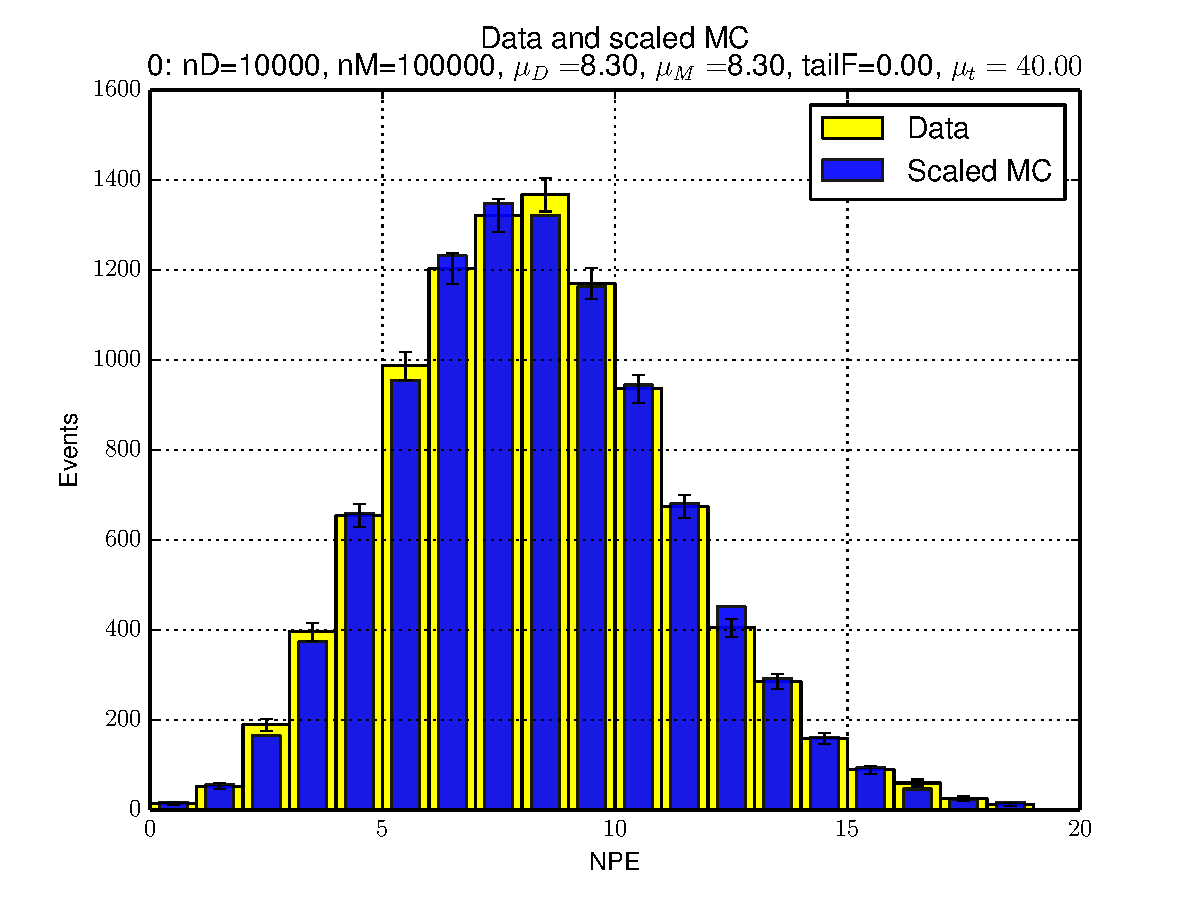
\includegraphics[width=0.45\textwidth]{../FIGURES/00/FIG_Data_and_scaled_MC.pdf} 
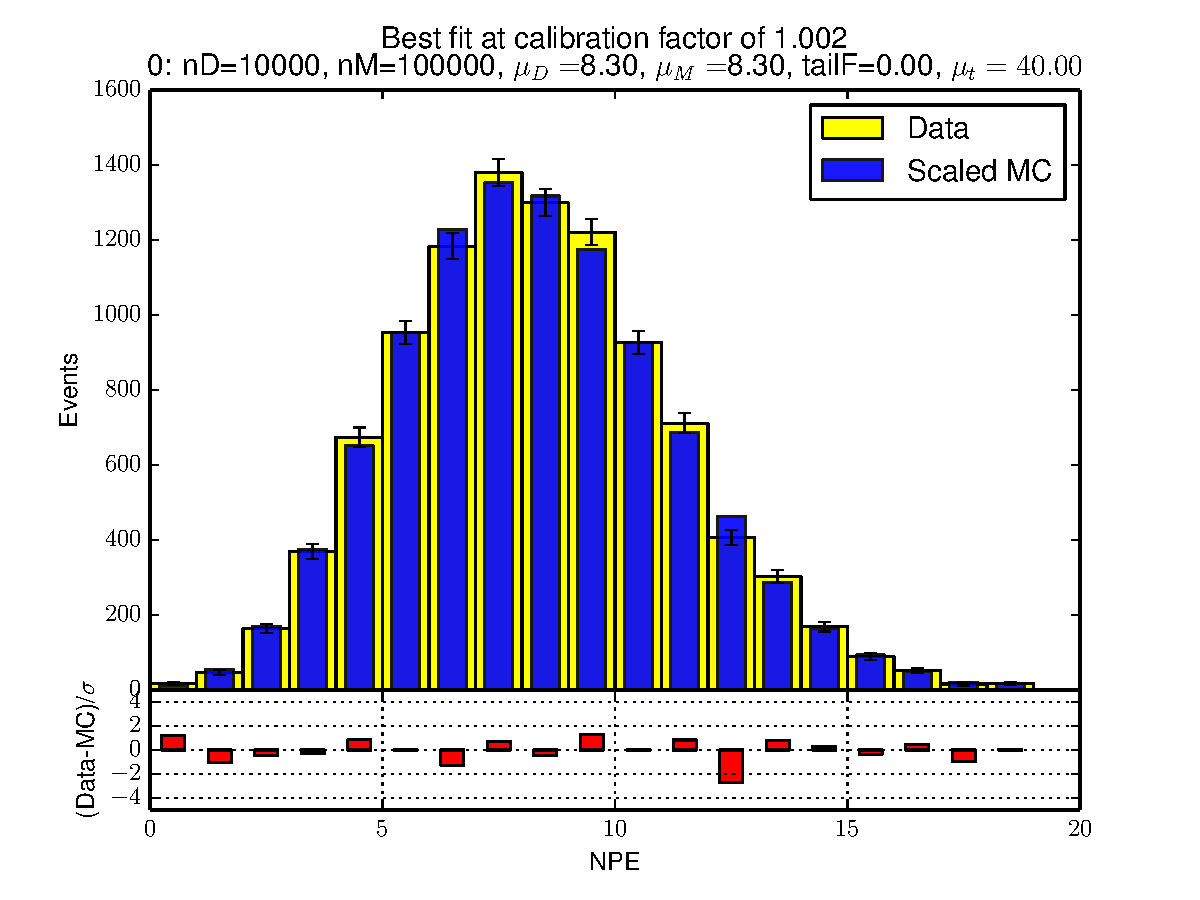
\includegraphics[width=0.45\textwidth]{../FIGURES/00/FIG_Best_fit_at_calibration_factor_of_1_002.pdf} 
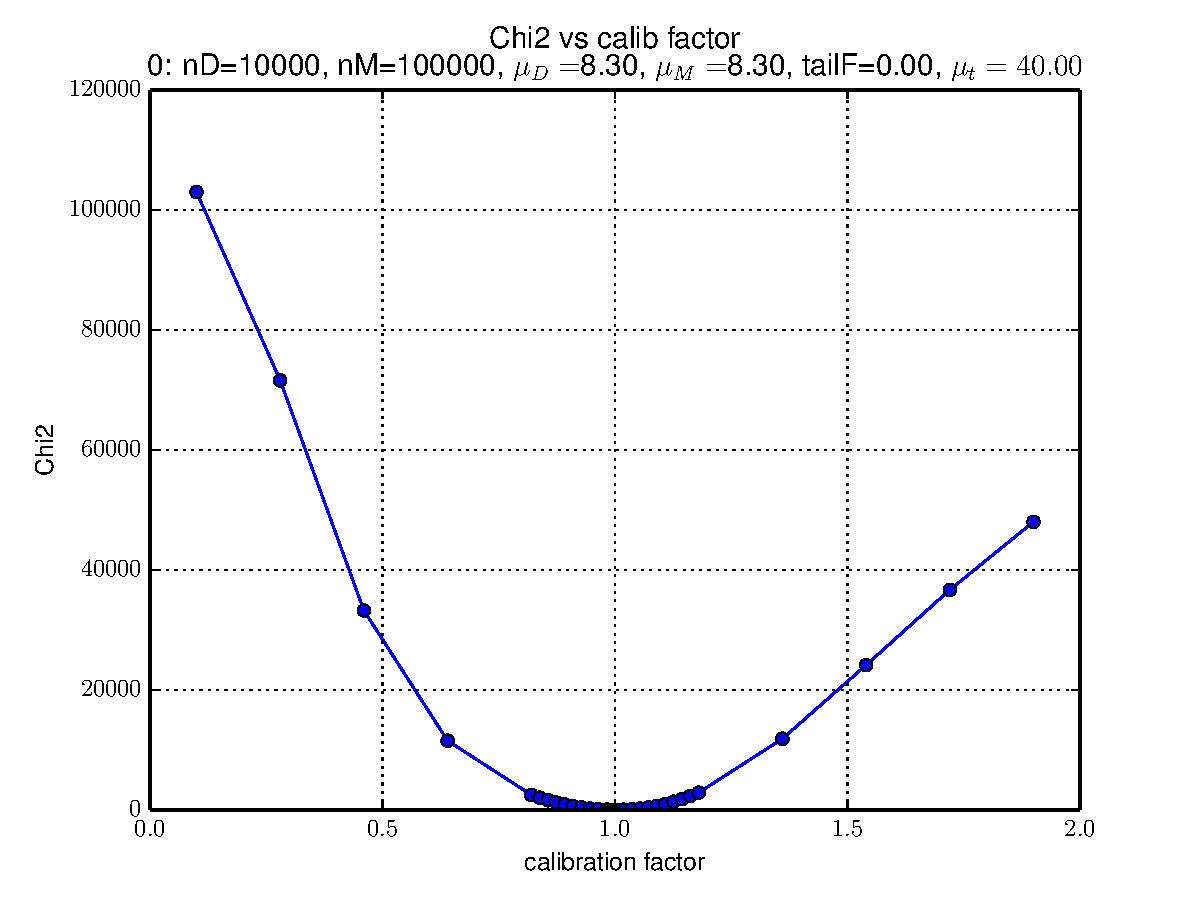
\includegraphics[width=0.45\textwidth]{../FIGURES/00/FIG_Chi2_vs_calib_factor.pdf} 
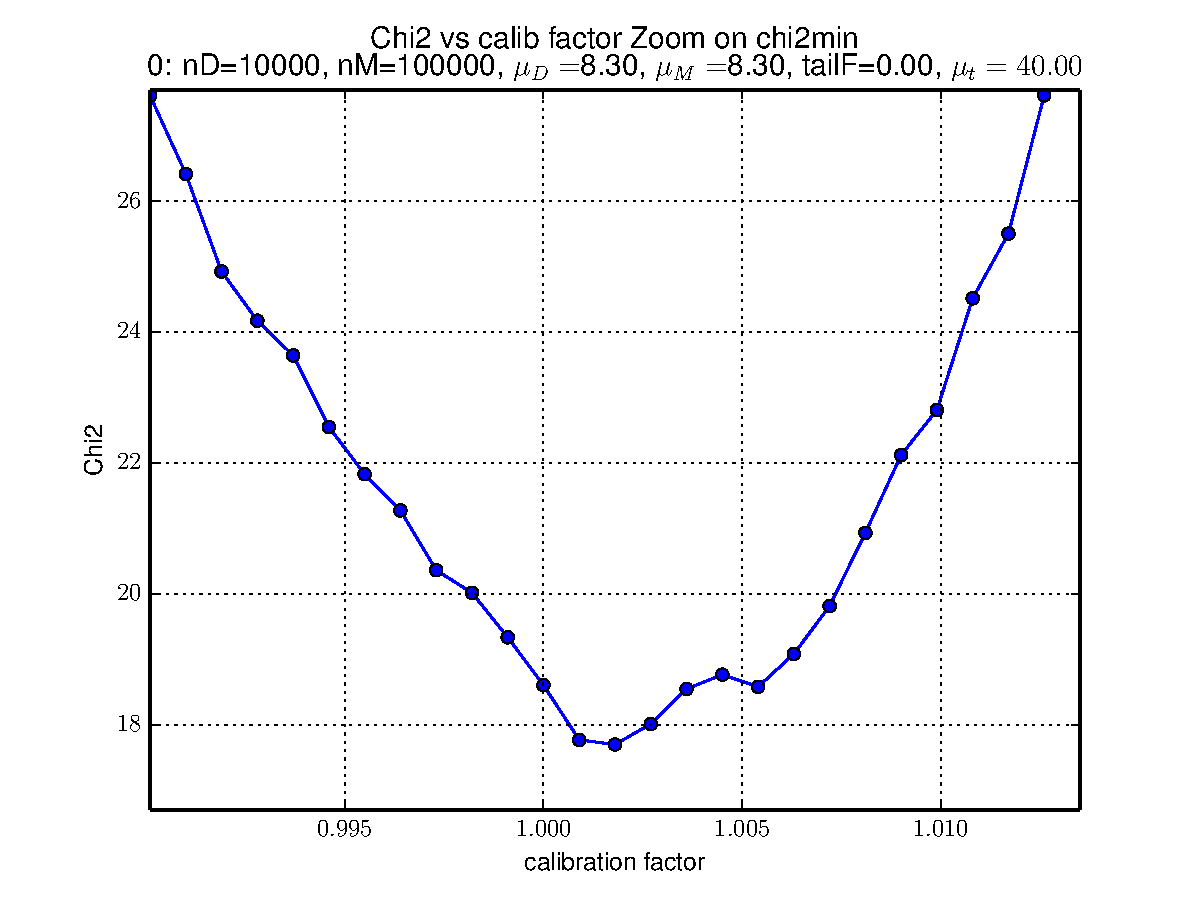
\includegraphics[width=0.45\textwidth]{../FIGURES/00/FIG_Chi2_vs_calib_factor_Zoom_on_chi2min.pdf} 
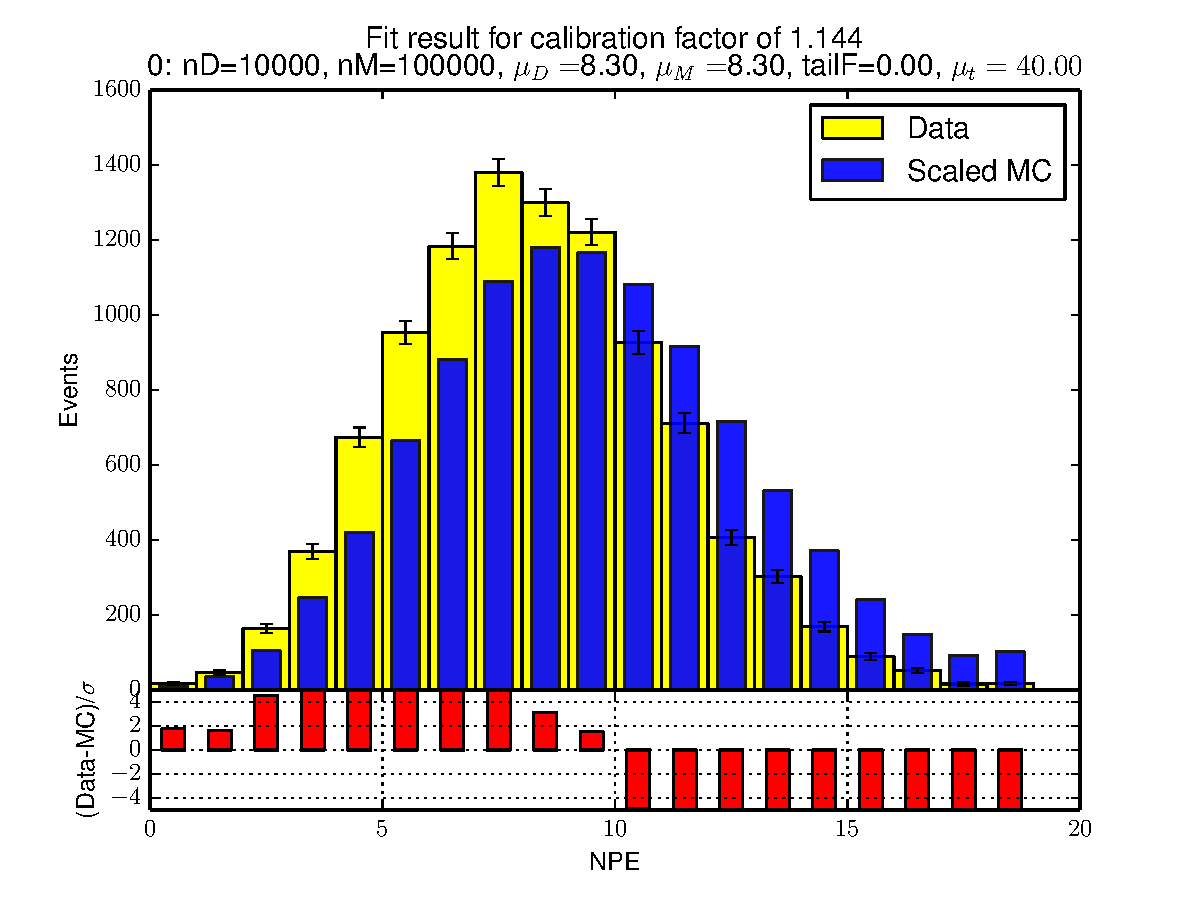
\includegraphics[width=0.45\textwidth]{../FIGURES/00/FIG_Fit_result_for_calibration_factor_of_1_144.pdf} 
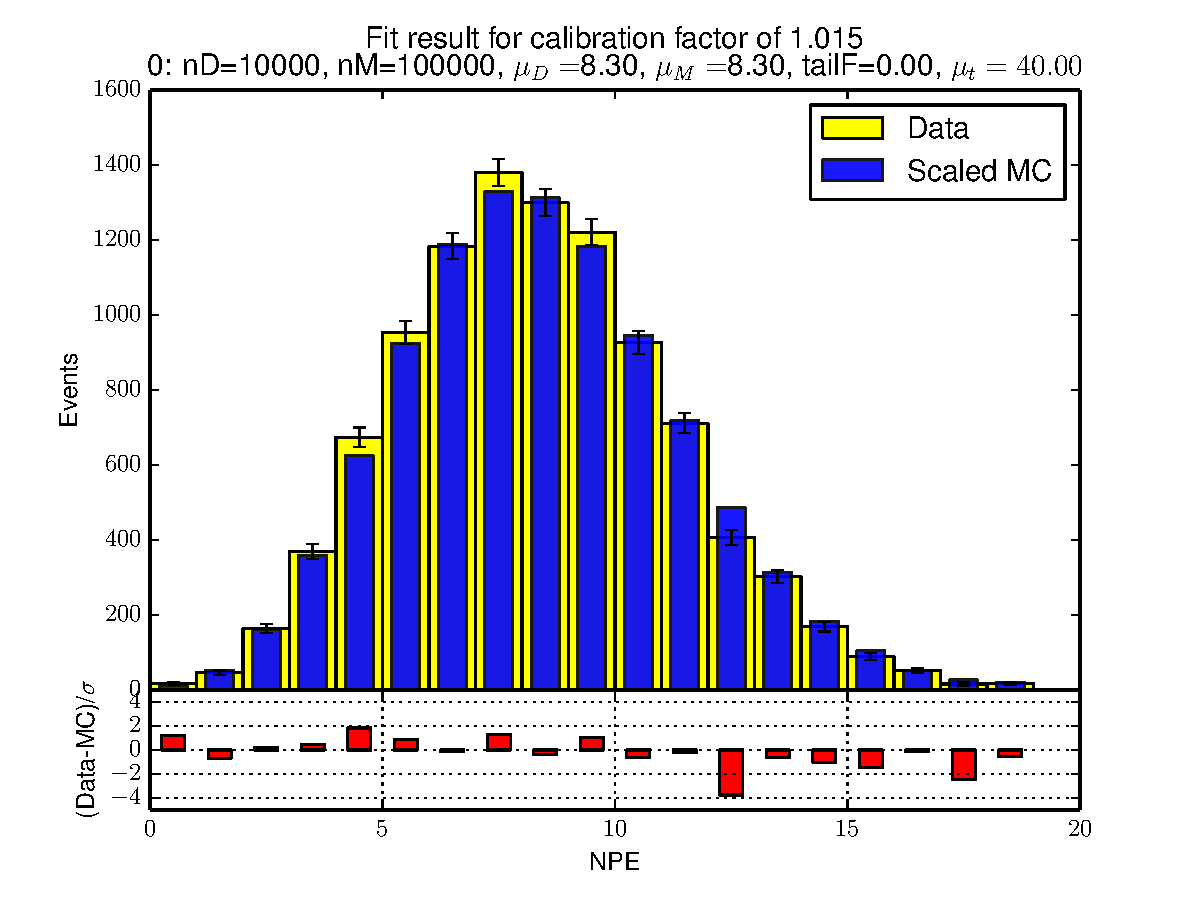
\includegraphics[width=0.45\textwidth]{../FIGURES/00/FIG_Fit_result_for_calibration_factor_of_1_015.pdf} 
\caption{Data compared to nominal MC, MC scaled by the best fit calibration factor, scans of $\chi^2$ over a large range and about the minimum for configuration 00. Data compared to MC scaled by two randomly chosen calibration factors.} 
\label{tab:best_00} 
\end{center} \end{figure} 

 \begin{figure}[htbp] \begin{center} 
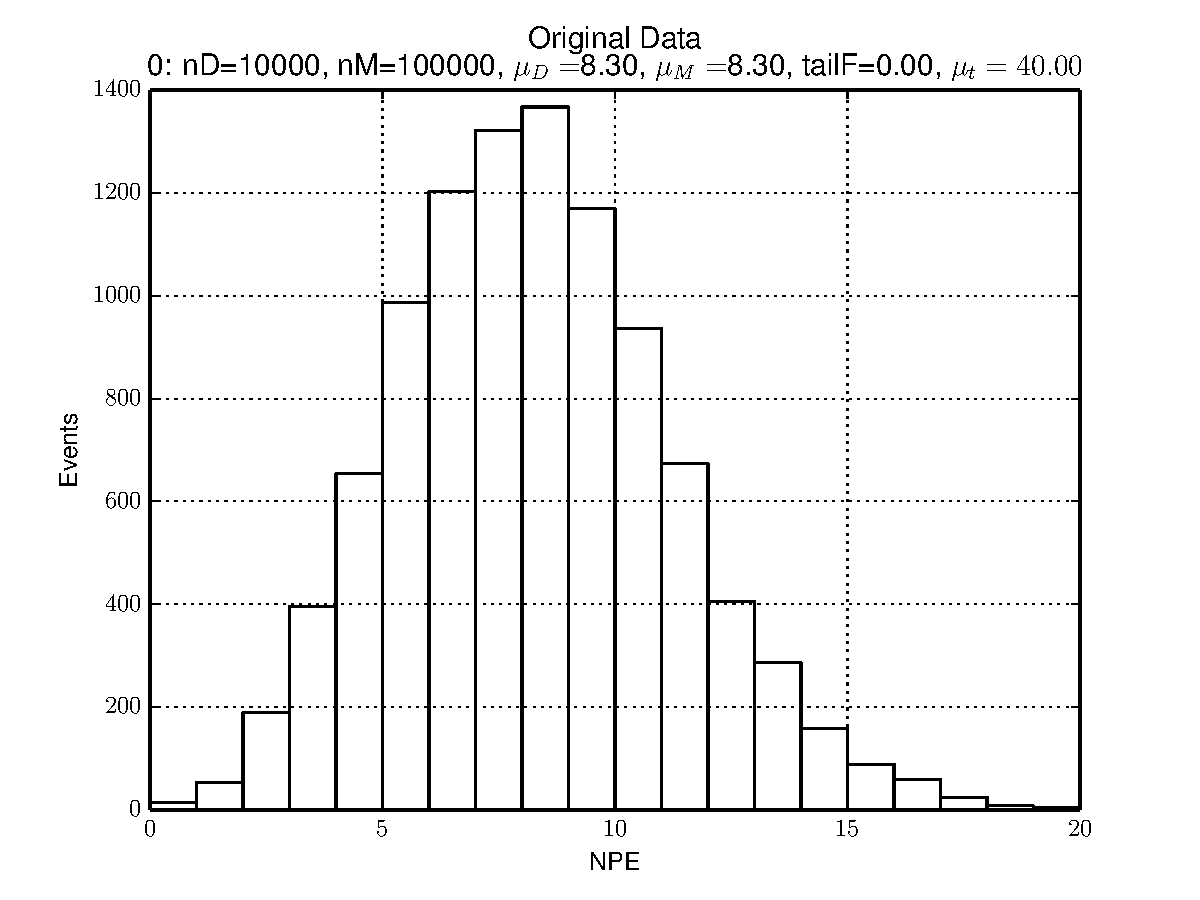
\includegraphics[width=0.45\textwidth]{../FIGURES/00/FIG_Original_Data.pdf} 
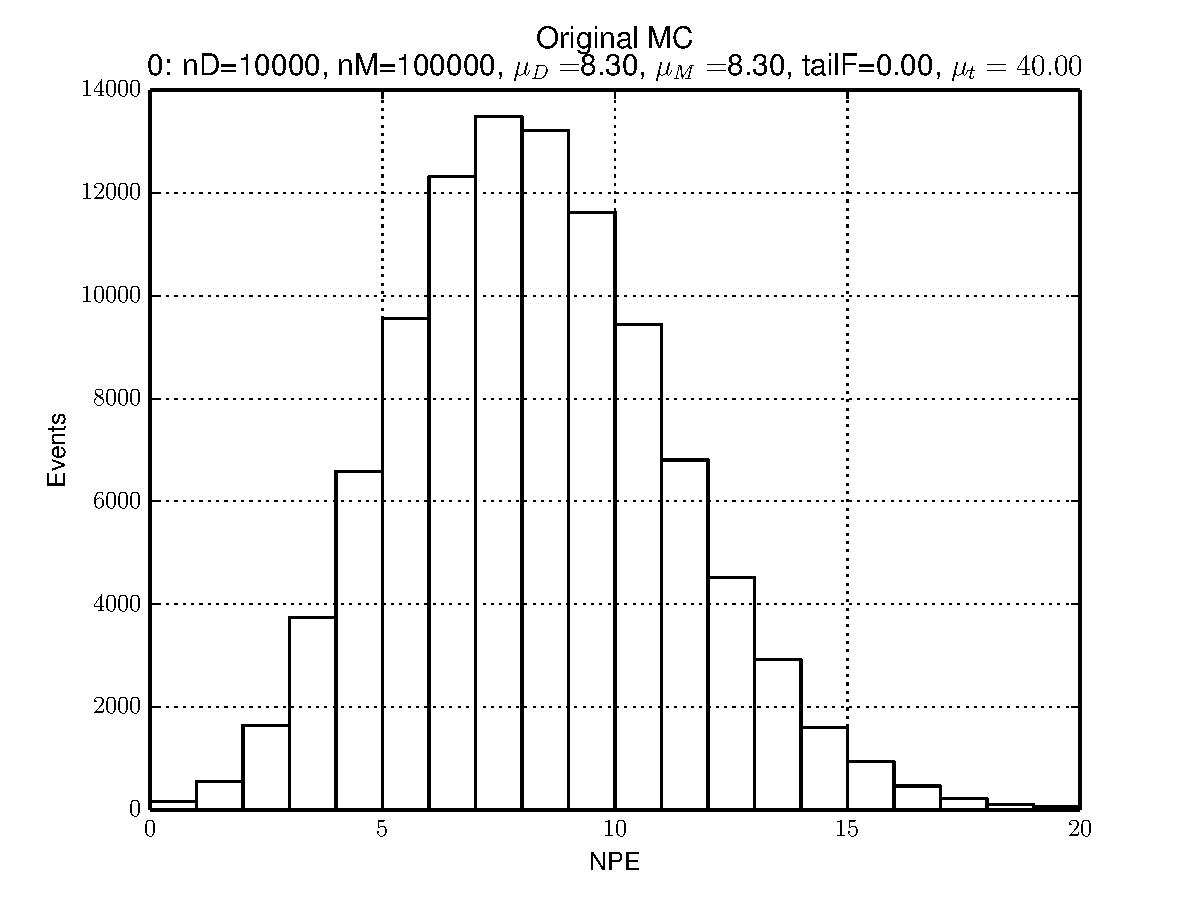
\includegraphics[width=0.45\textwidth]{../FIGURES/00/FIG_Original_MC.pdf} 
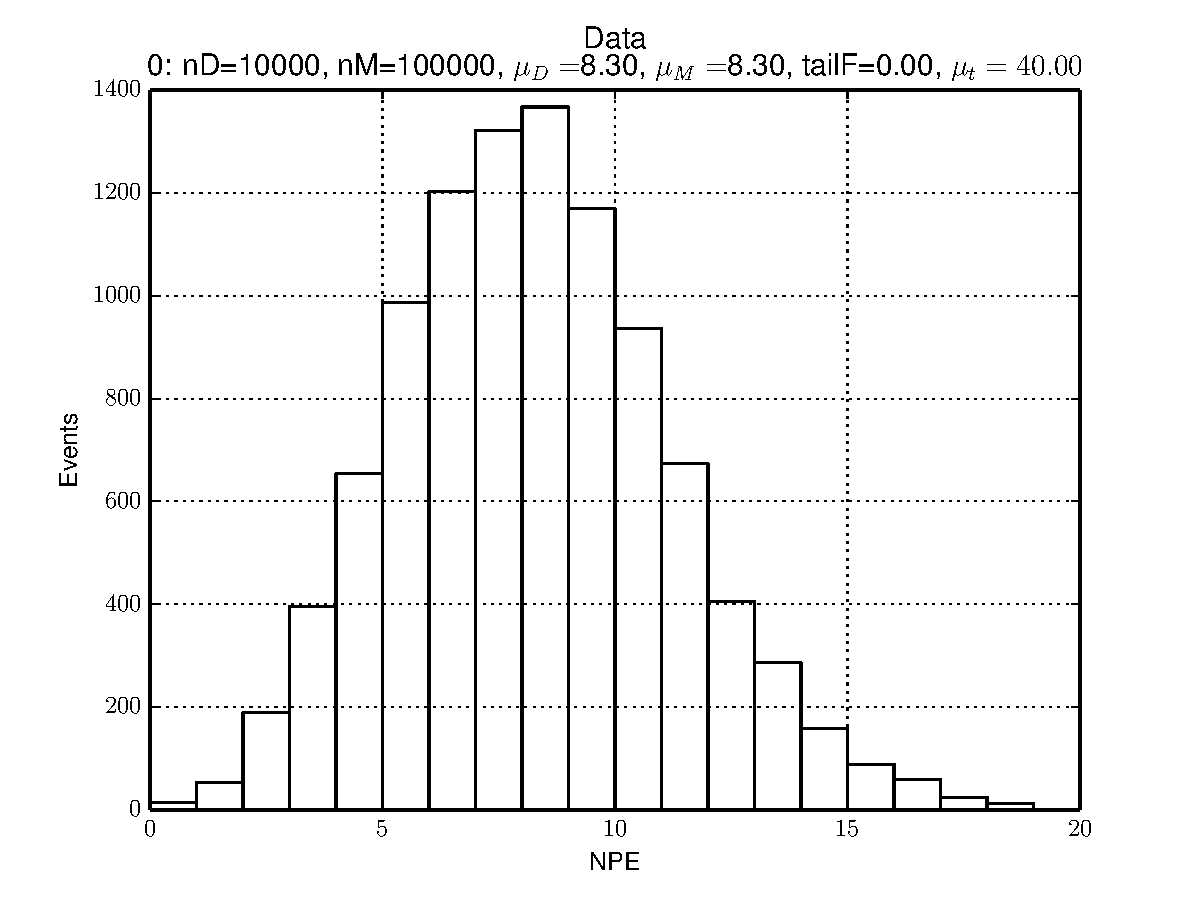
\includegraphics[width=0.45\textwidth]{../FIGURES/00/FIG_Data.pdf} 
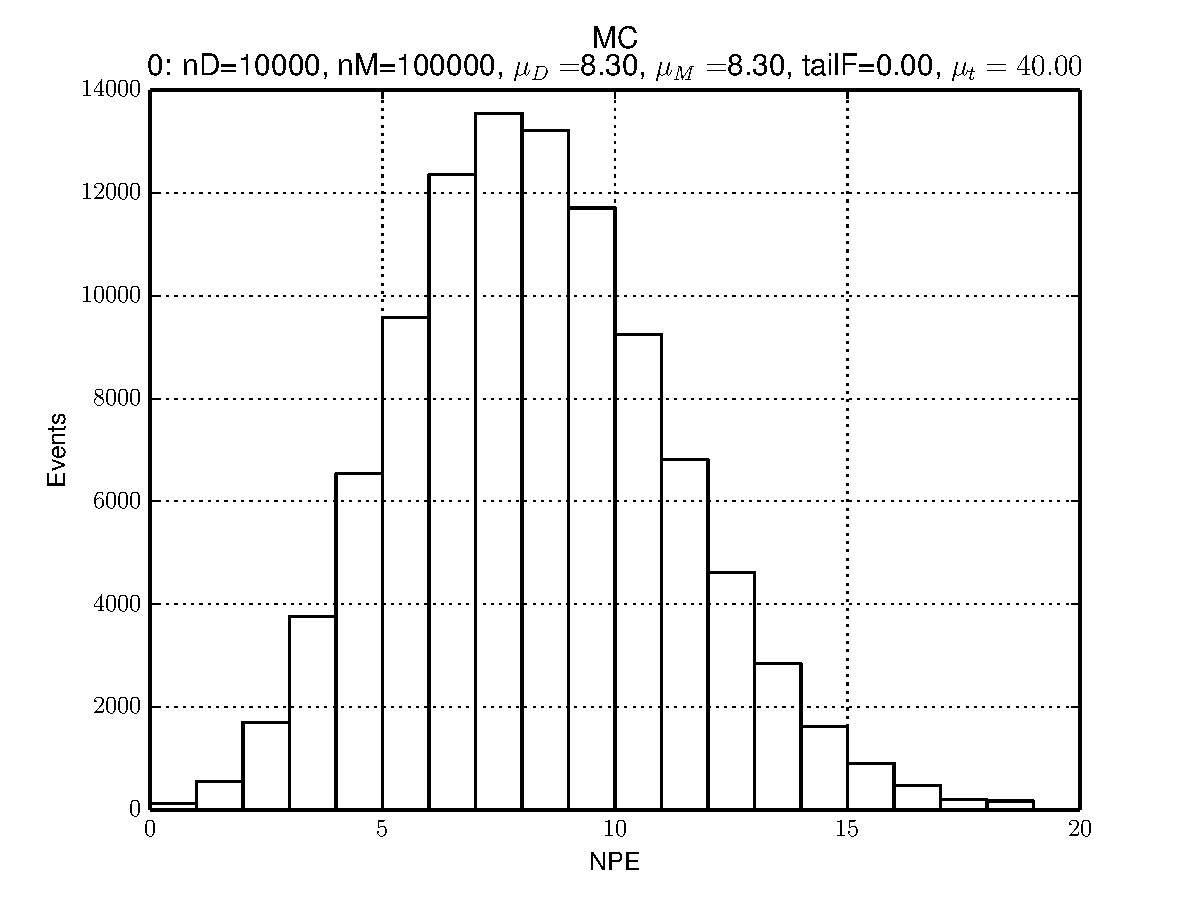
\includegraphics[width=0.45\textwidth]{../FIGURES/00/FIG_MC.pdf} 
\caption{NPE histograms for data and MC for configuration 00. Top are original hists. Bottom are hists after truncation at bin containing less than 10 entries with that bin containing overflows.} 
\label{tab:npe_00} 
\end{center} \end{figure} 

  \clearpage

 \begin{figure}[htbp] \begin{center} 
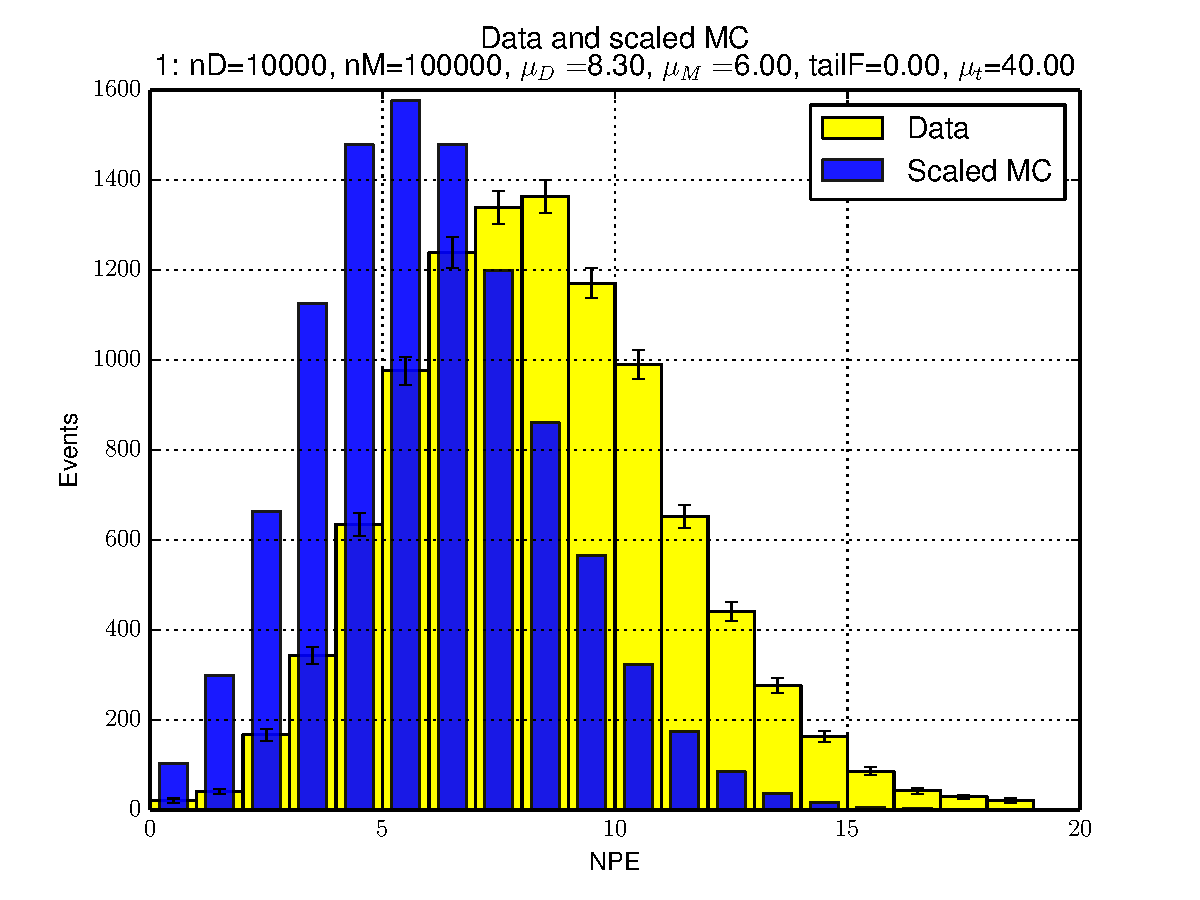
\includegraphics[width=0.45\textwidth]{../FIGURES/01/FIG_Data_and_scaled_MC.pdf} 
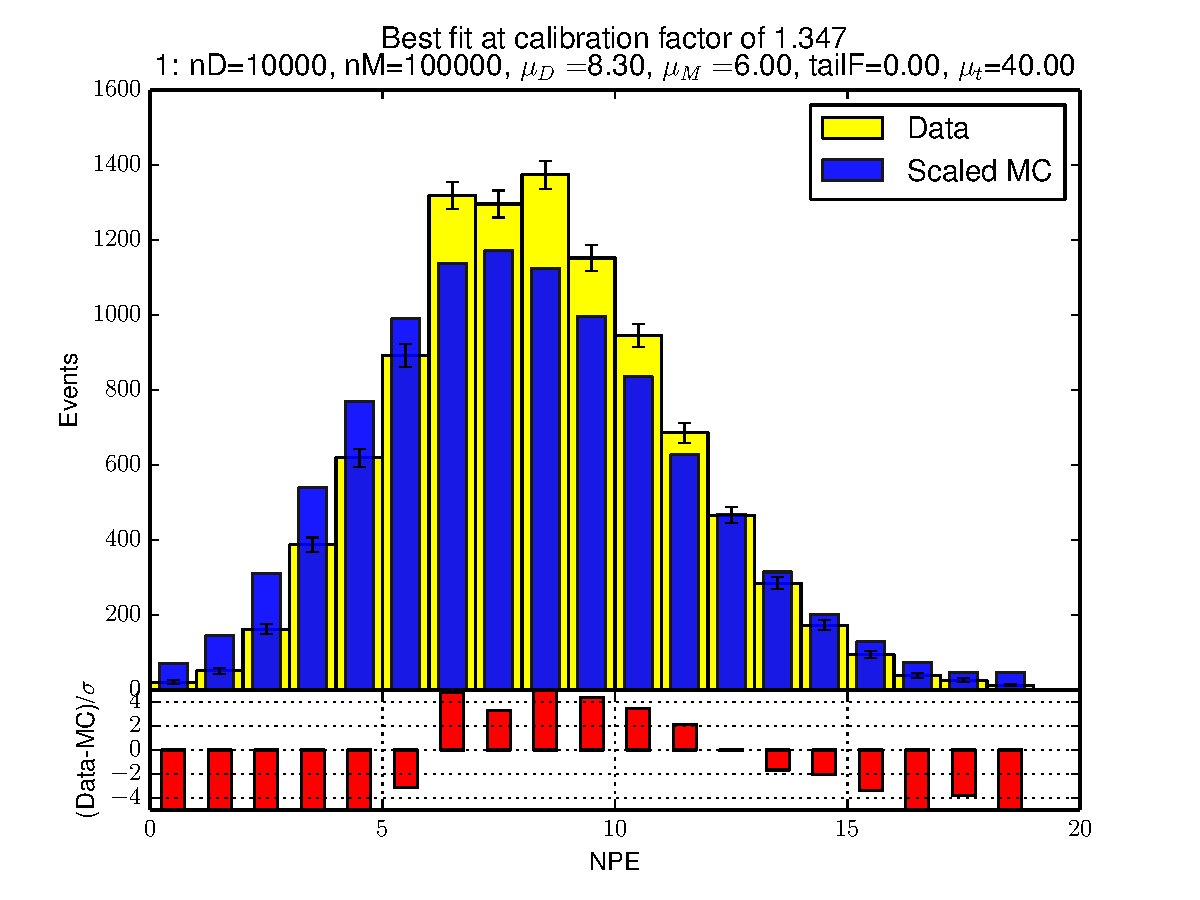
\includegraphics[width=0.45\textwidth]{../FIGURES/01/FIG_Best_fit_at_calibration_factor_of_1_347.pdf} 
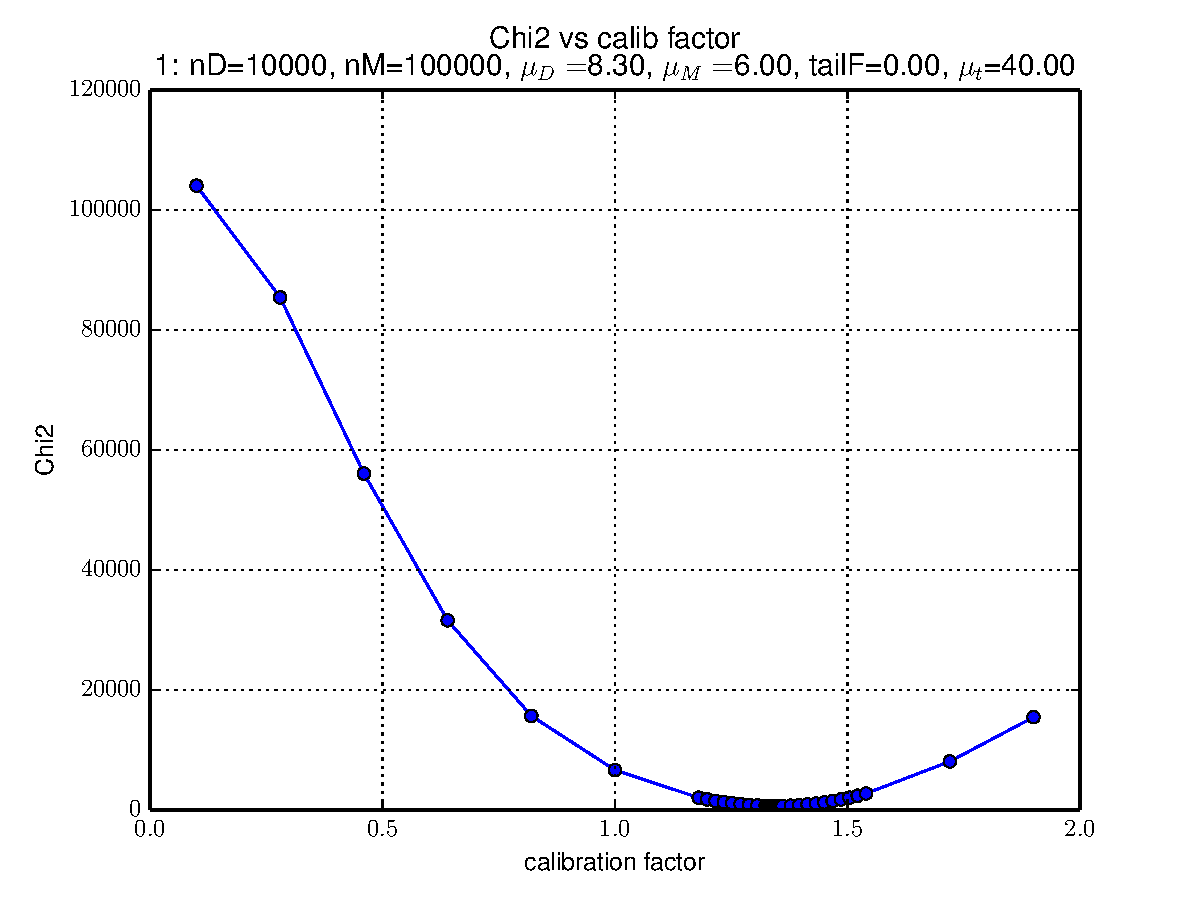
\includegraphics[width=0.45\textwidth]{../FIGURES/01/FIG_Chi2_vs_calib_factor.pdf} 
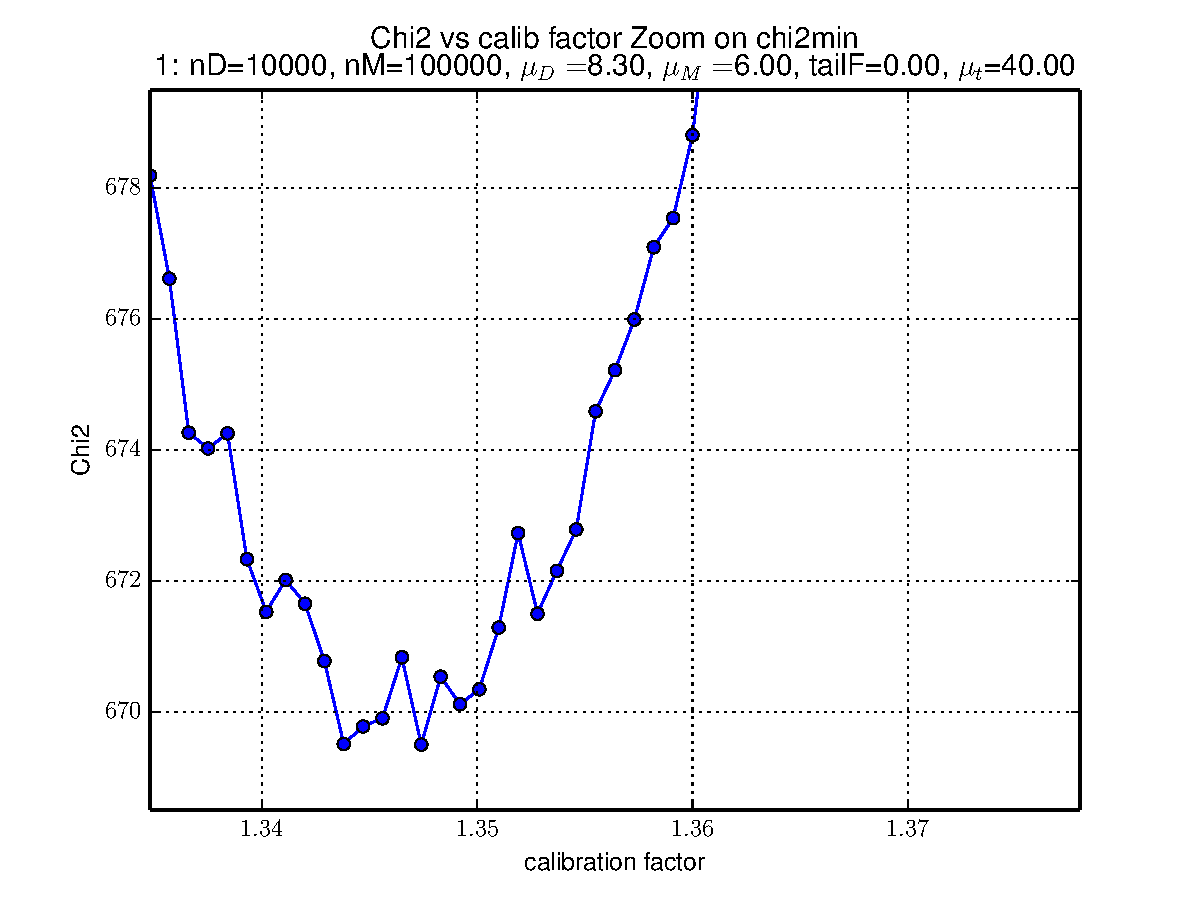
\includegraphics[width=0.45\textwidth]{../FIGURES/01/FIG_Chi2_vs_calib_factor_Zoom_on_chi2min.pdf} 
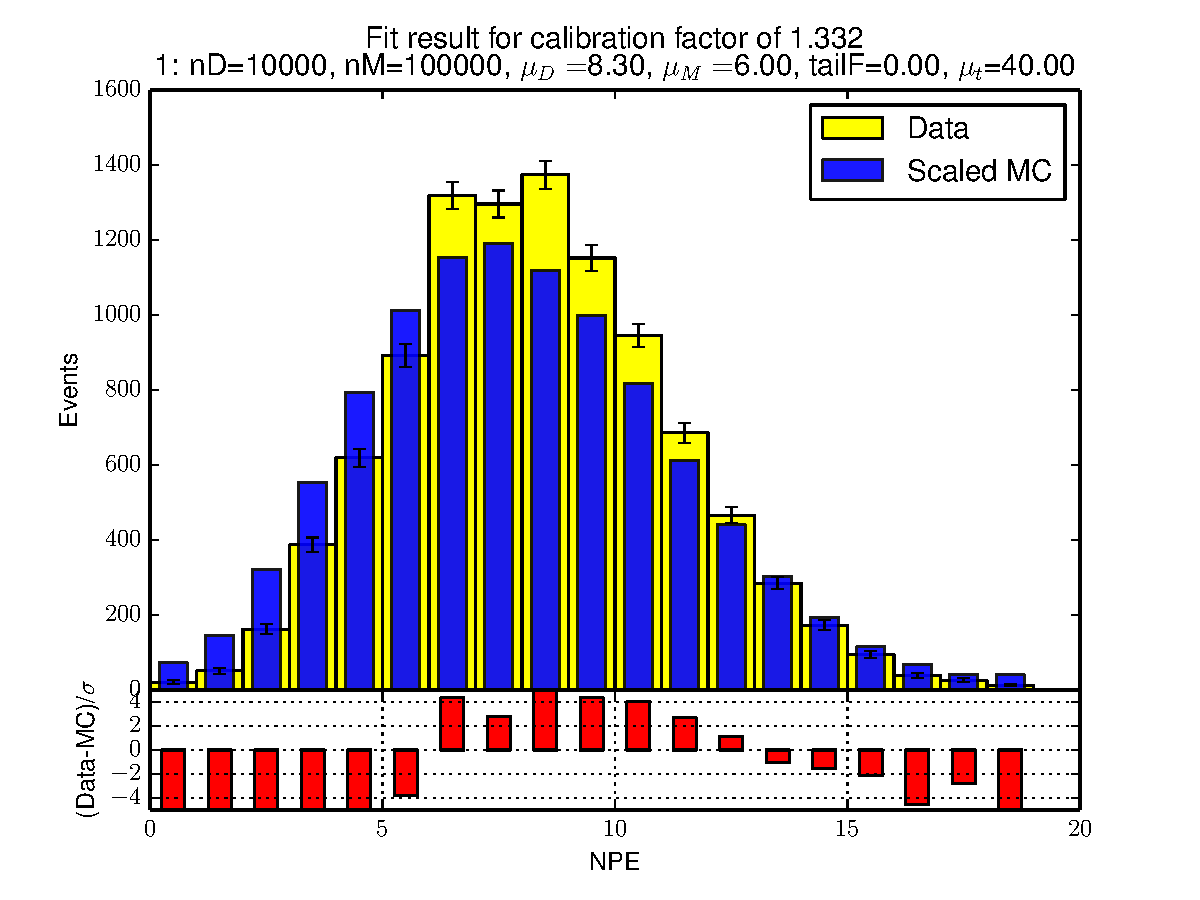
\includegraphics[width=0.45\textwidth]{../FIGURES/01/FIG_Fit_result_for_calibration_factor_of_1_332.pdf} 
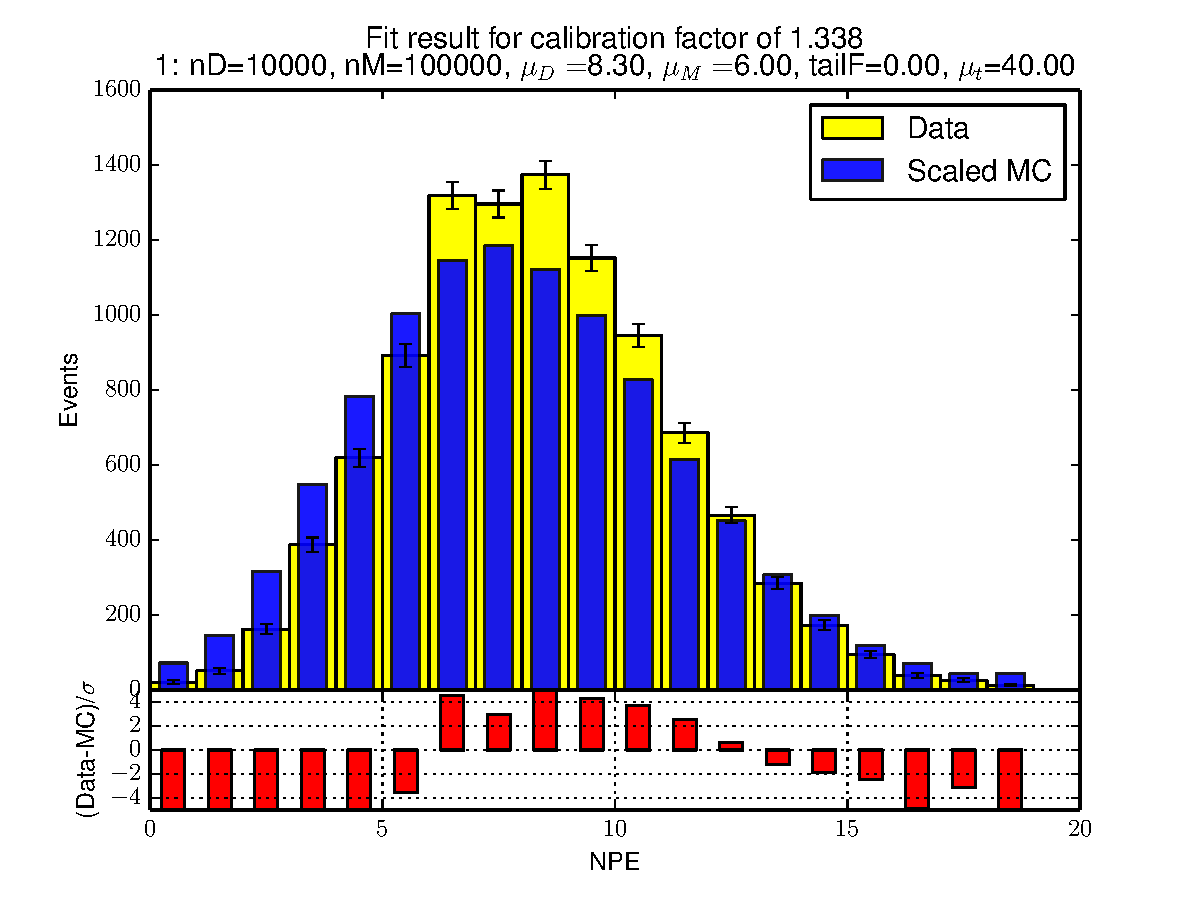
\includegraphics[width=0.45\textwidth]{../FIGURES/01/FIG_Fit_result_for_calibration_factor_of_1_338.pdf} 
\caption{Data compared to nominal MC, MC scaled by the best fit calibration factor, scans of $\chi^2$ over a large range and about the minimum for configuration 01. Data compared to MC scaled by two randomly chosen calibration factors.} 
\label{tab:best_01} 
\end{center} \end{figure} 

 \begin{figure}[htbp] \begin{center} 
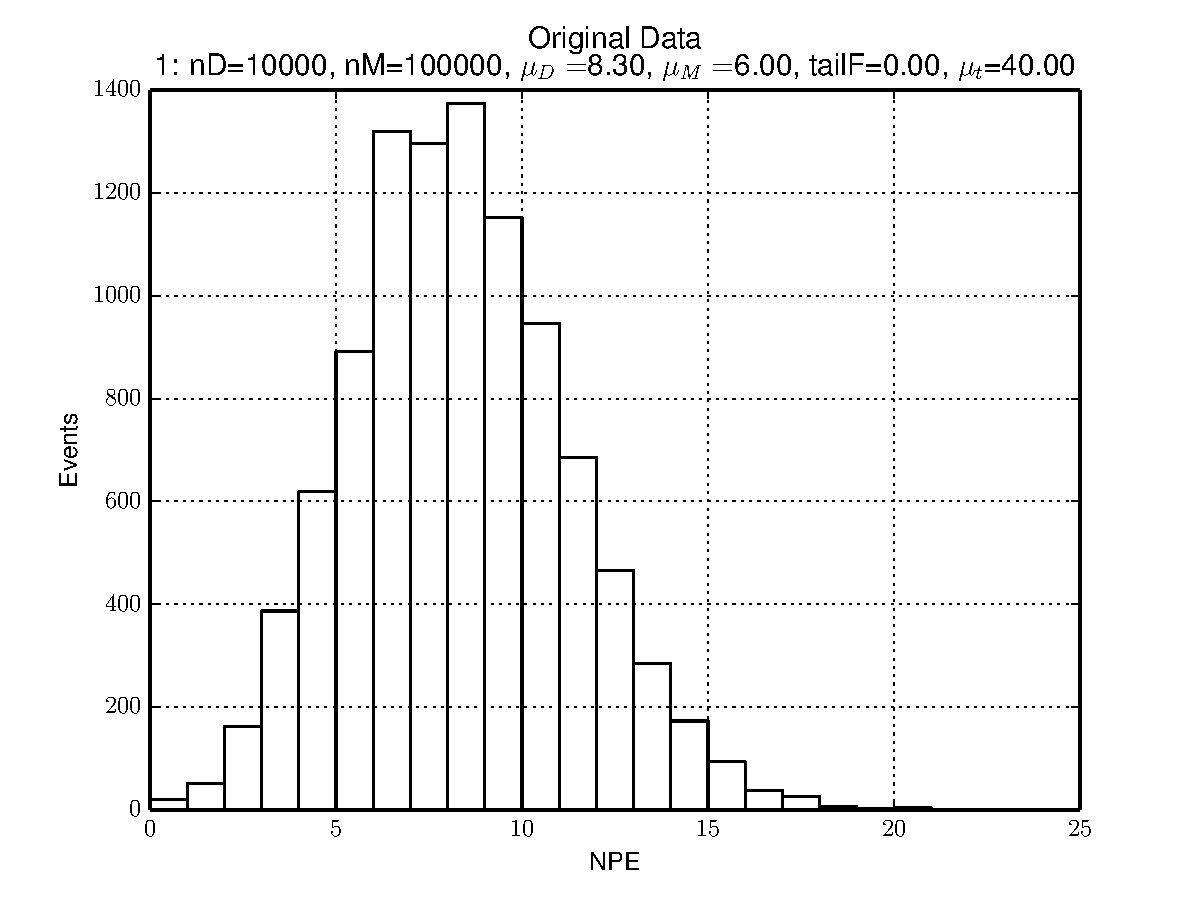
\includegraphics[width=0.45\textwidth]{../FIGURES/01/FIG_Original_Data.pdf} 
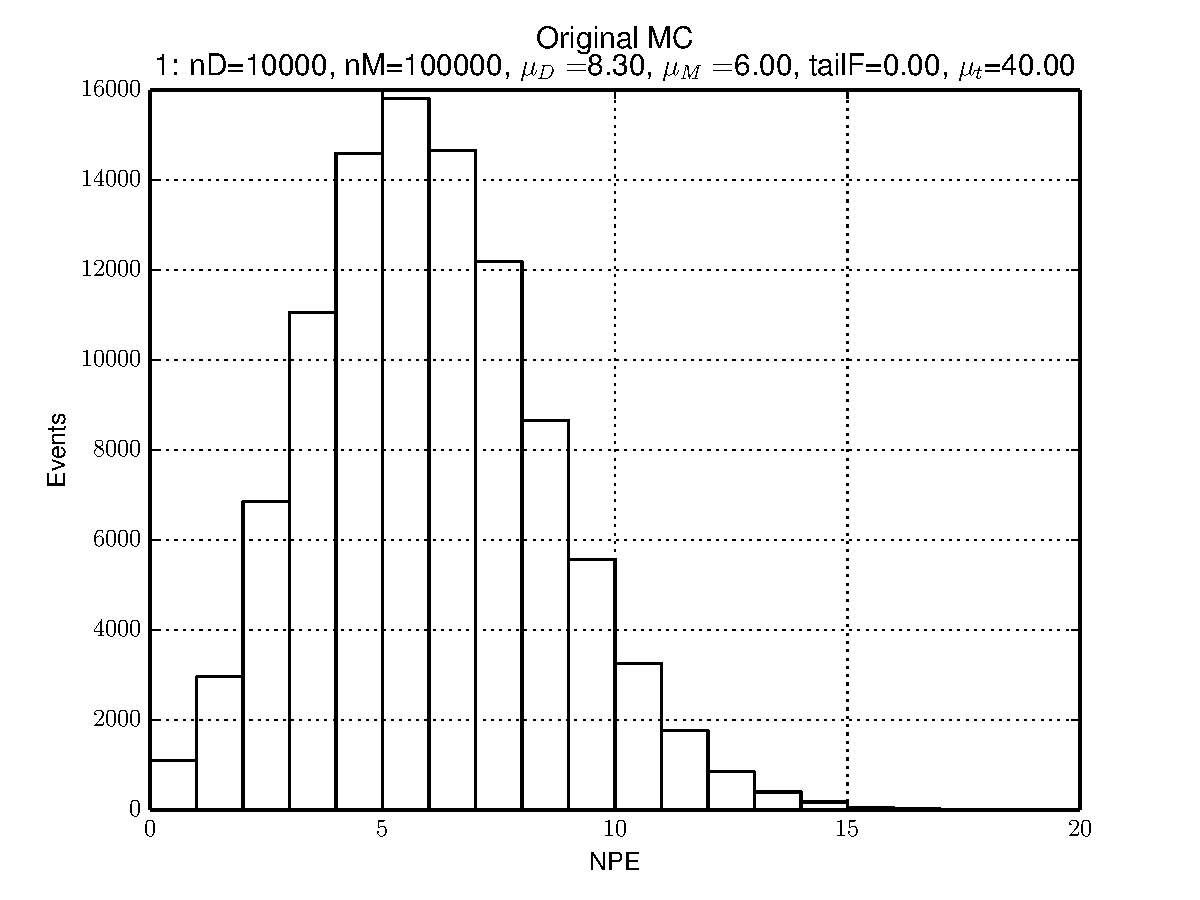
\includegraphics[width=0.45\textwidth]{../FIGURES/01/FIG_Original_MC.pdf} 
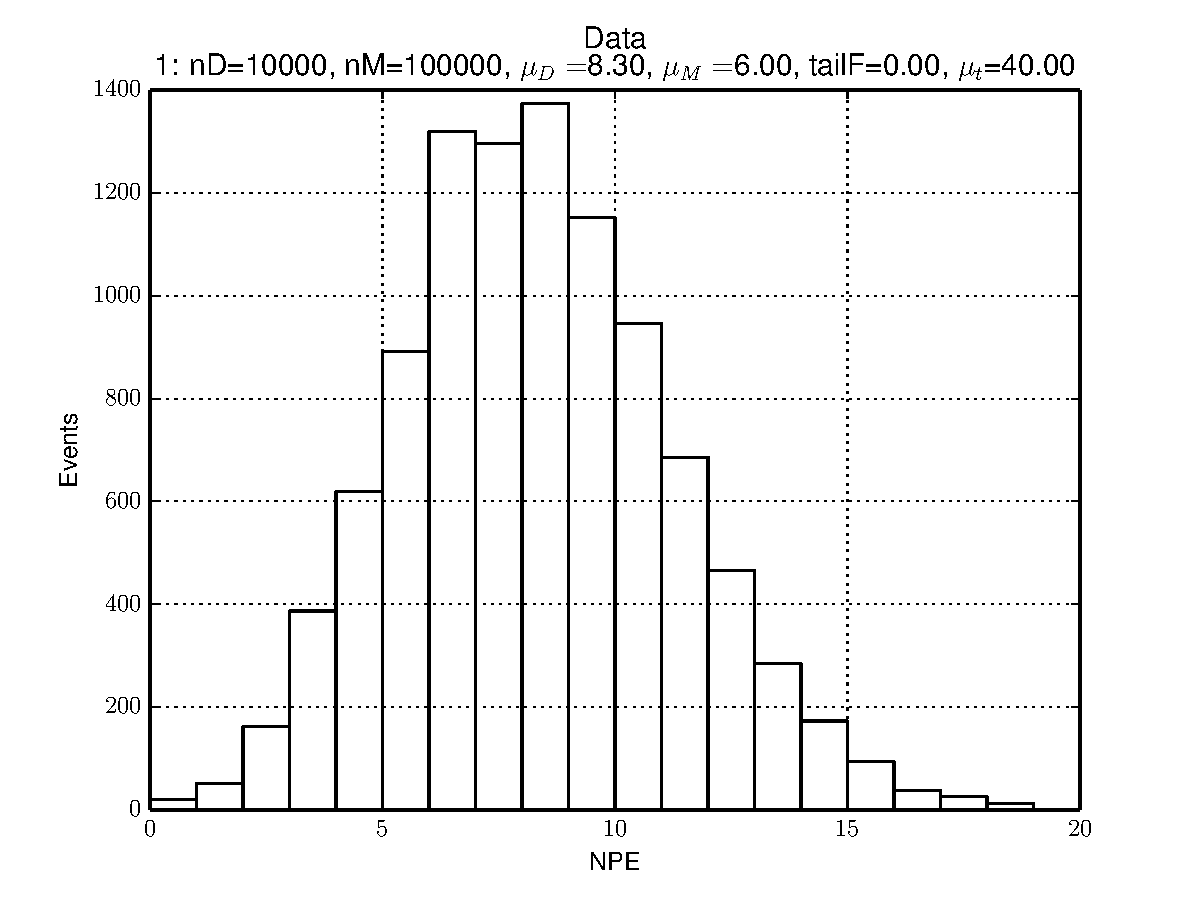
\includegraphics[width=0.45\textwidth]{../FIGURES/01/FIG_Data.pdf} 
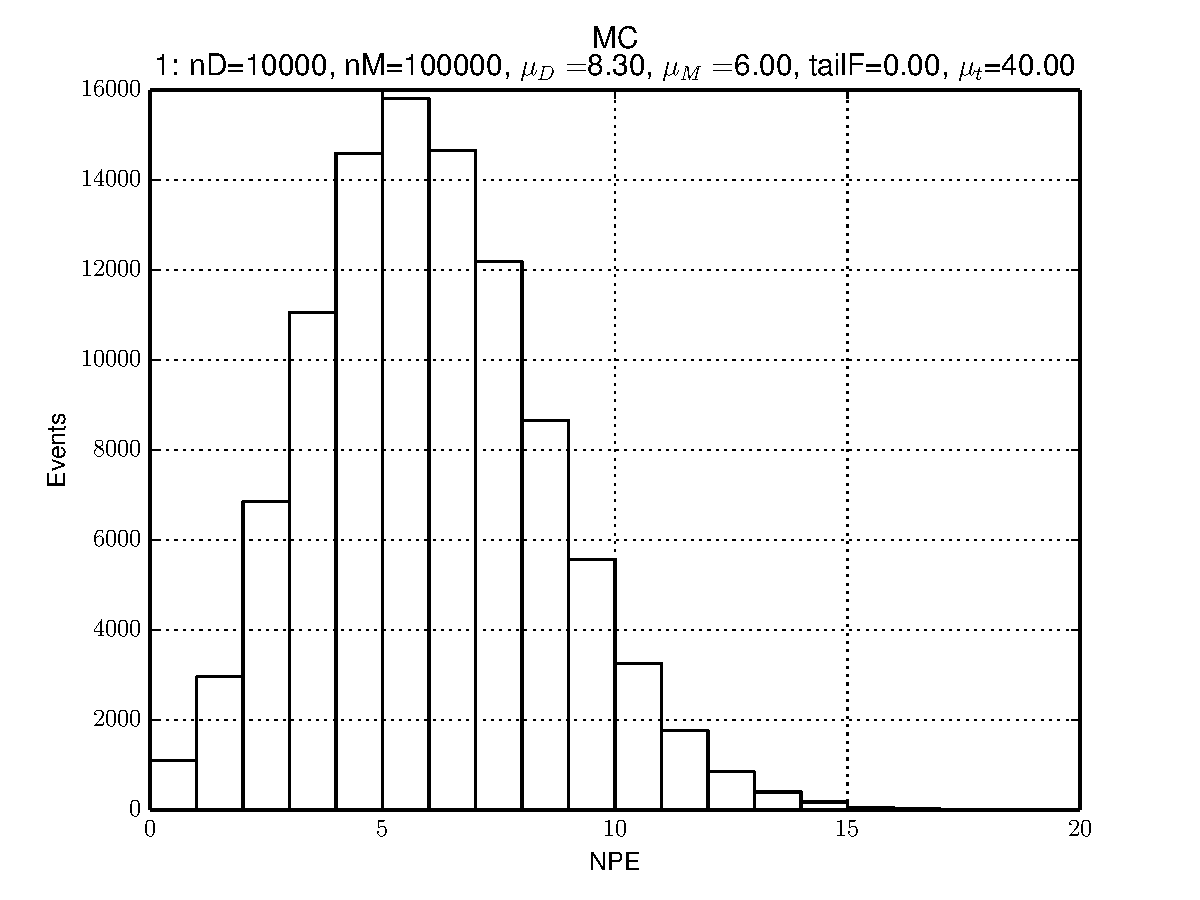
\includegraphics[width=0.45\textwidth]{../FIGURES/01/FIG_MC.pdf} 
\caption{NPE histograms for data and MC for configuration 01. Top are original hists. Bottom are hists after truncation at bin containing less than 10 entries with that bin containing overflows.} 
\label{tab:npe_01} 
\end{center} \end{figure} 

  \clearpage

 \begin{figure}[htbp] \begin{center} 
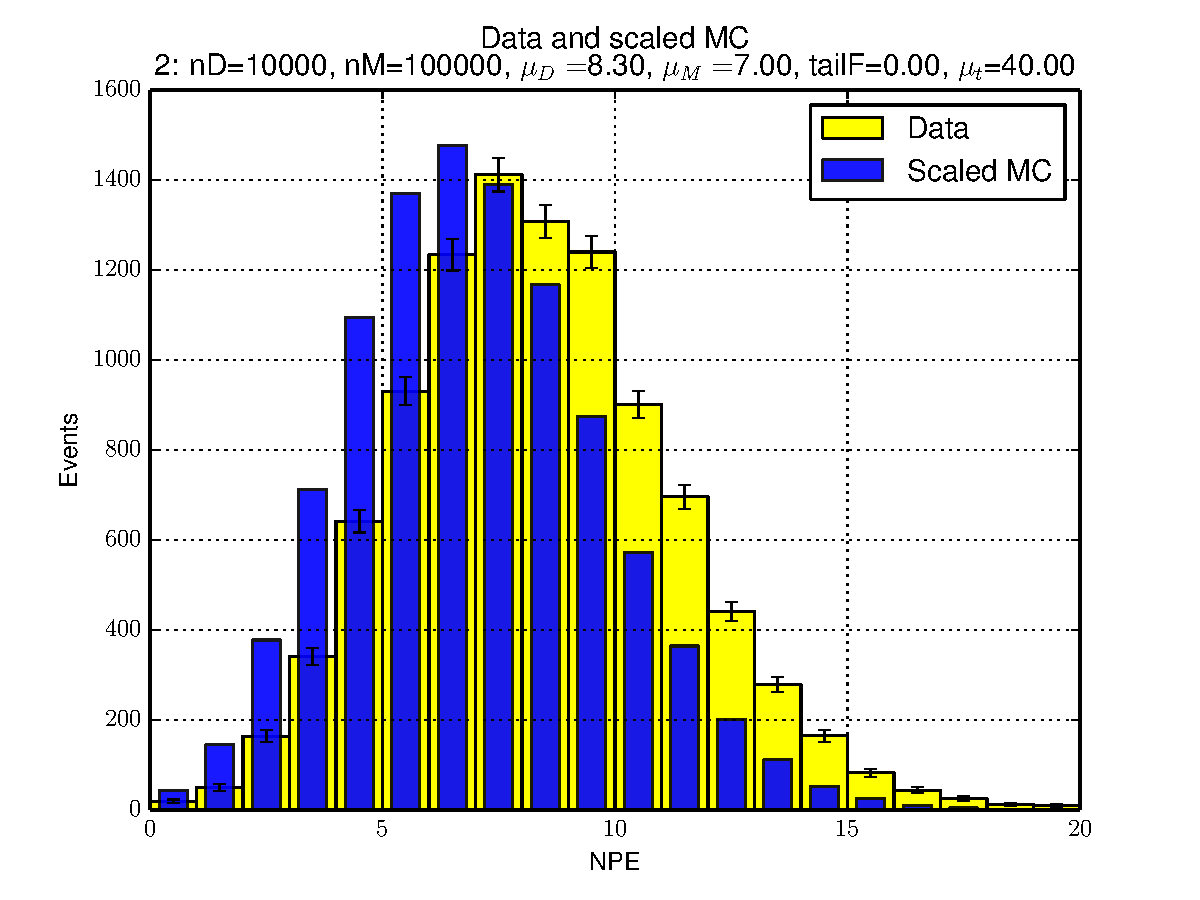
\includegraphics[width=0.45\textwidth]{../FIGURES/02/FIG_Data_and_scaled_MC.pdf} 
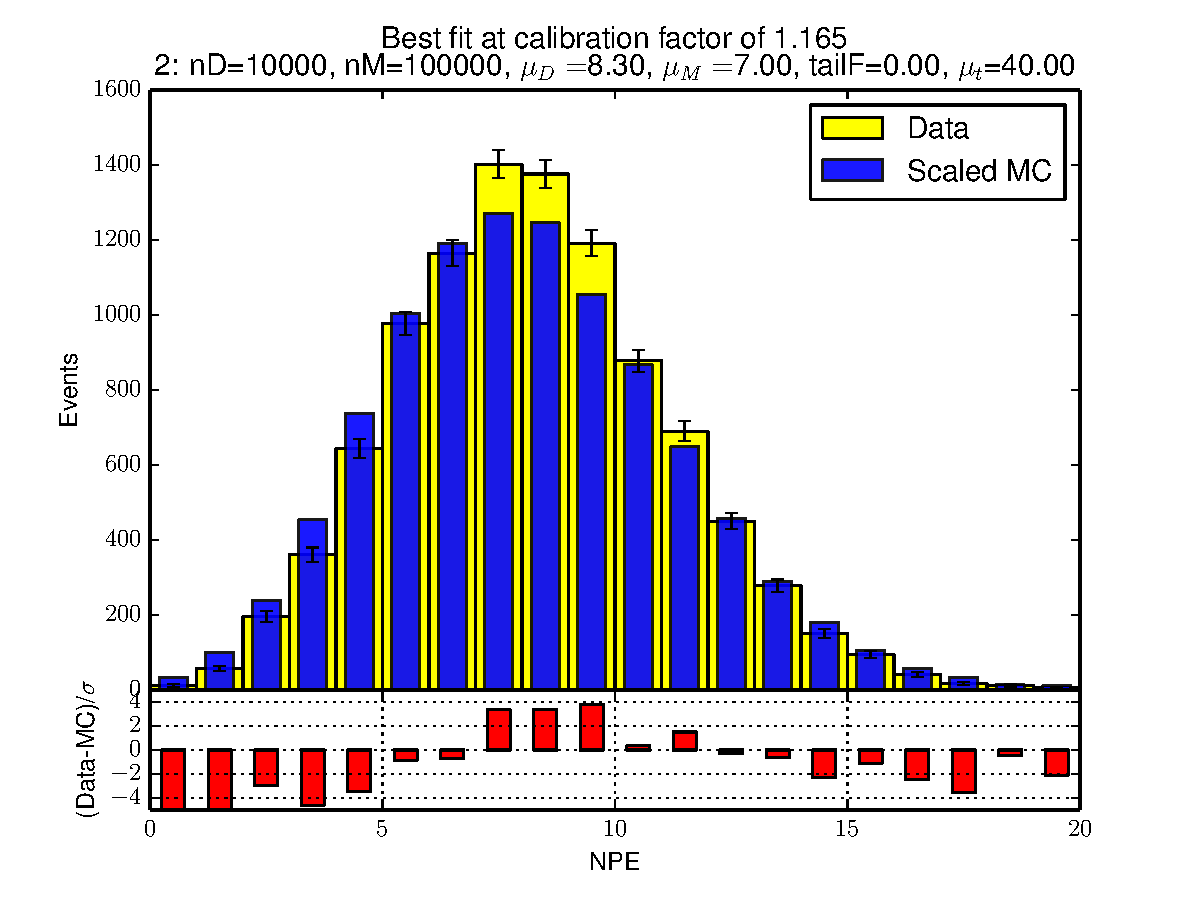
\includegraphics[width=0.45\textwidth]{../FIGURES/02/FIG_Best_fit_at_calibration_factor_of_1_165.pdf} 
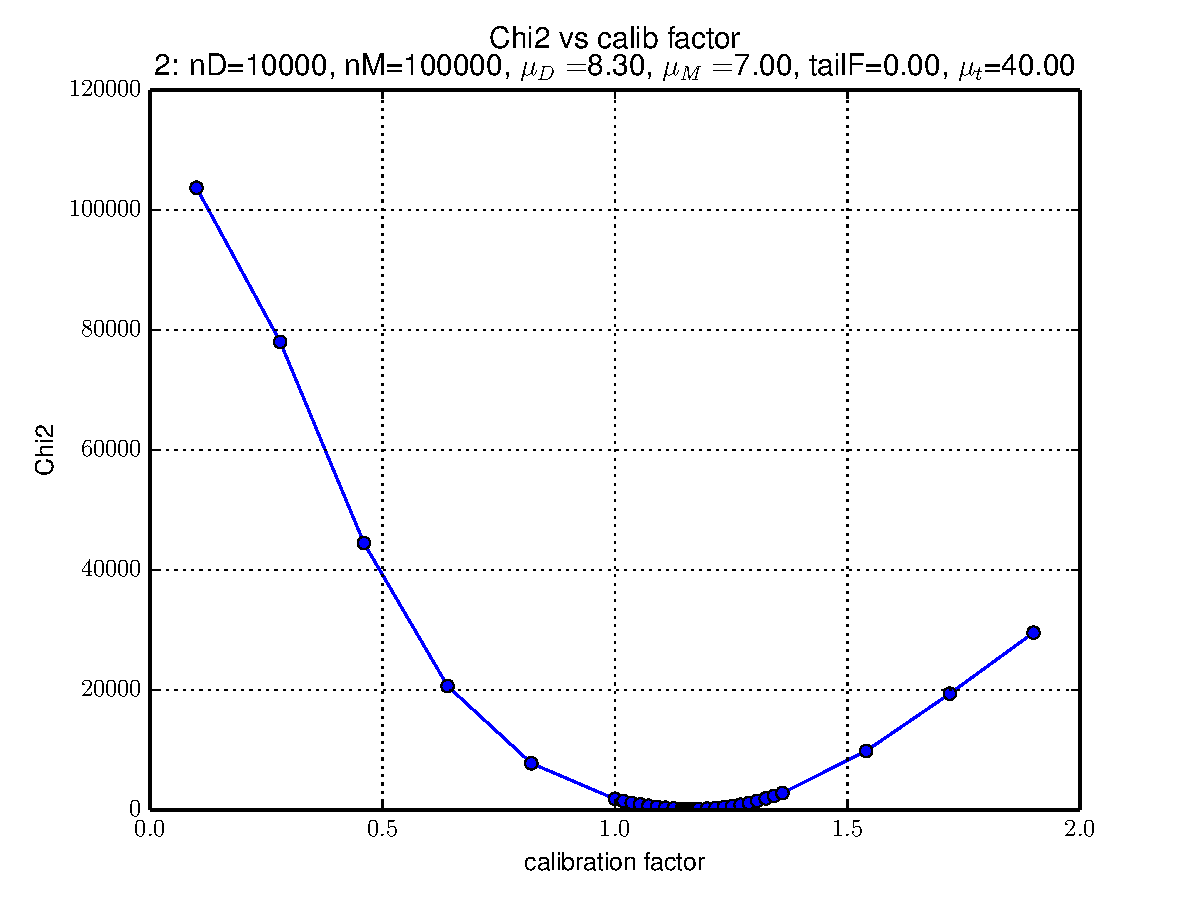
\includegraphics[width=0.45\textwidth]{../FIGURES/02/FIG_Chi2_vs_calib_factor.pdf} 
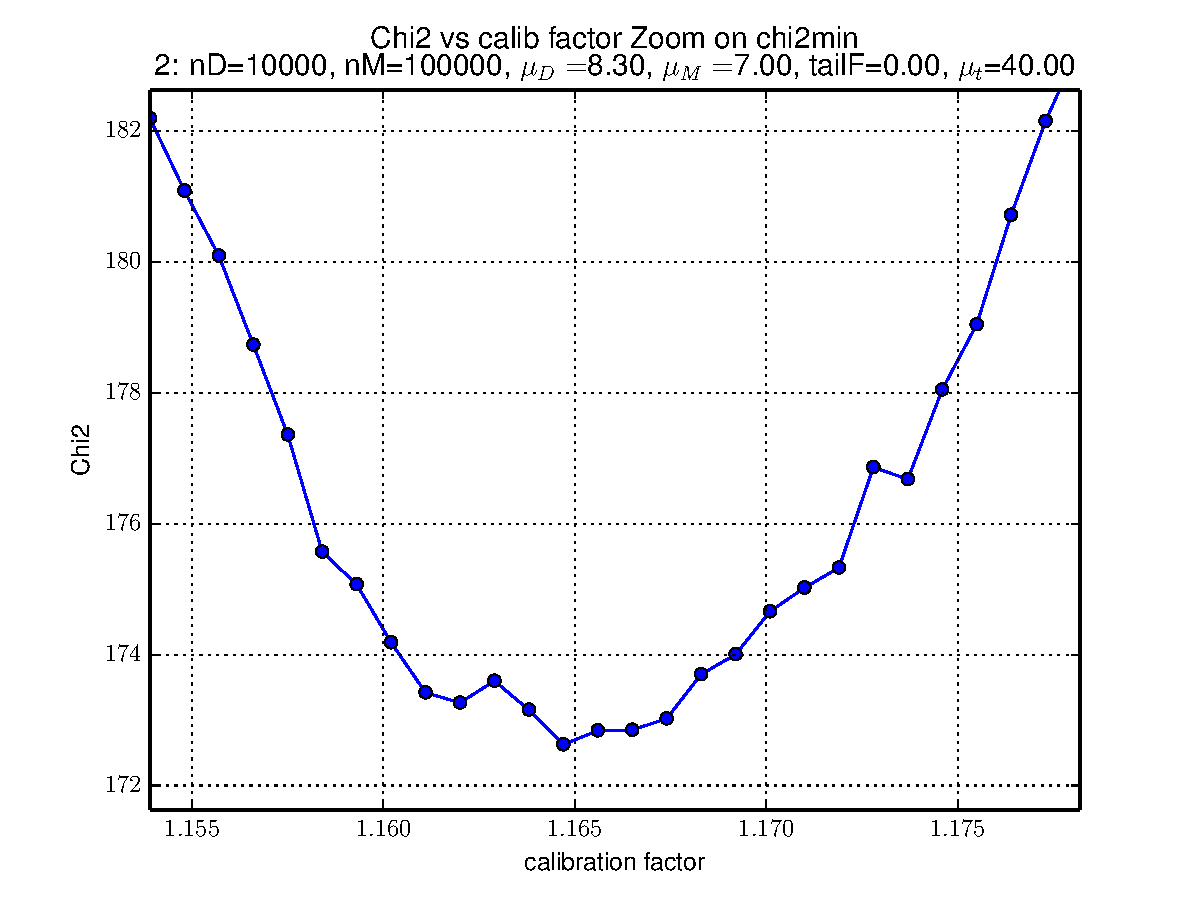
\includegraphics[width=0.45\textwidth]{../FIGURES/02/FIG_Chi2_vs_calib_factor_Zoom_on_chi2min.pdf} 
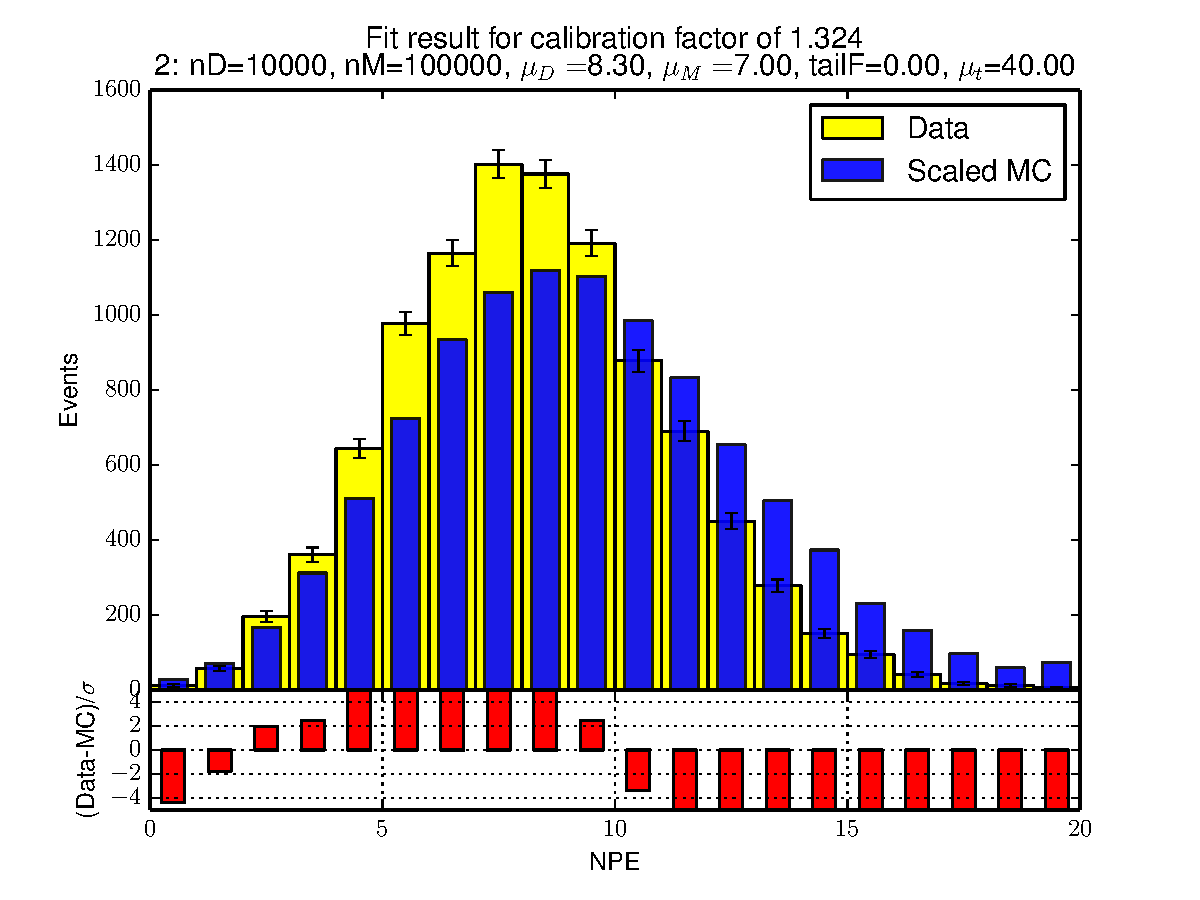
\includegraphics[width=0.45\textwidth]{../FIGURES/02/FIG_Fit_result_for_calibration_factor_of_1_324.pdf} 
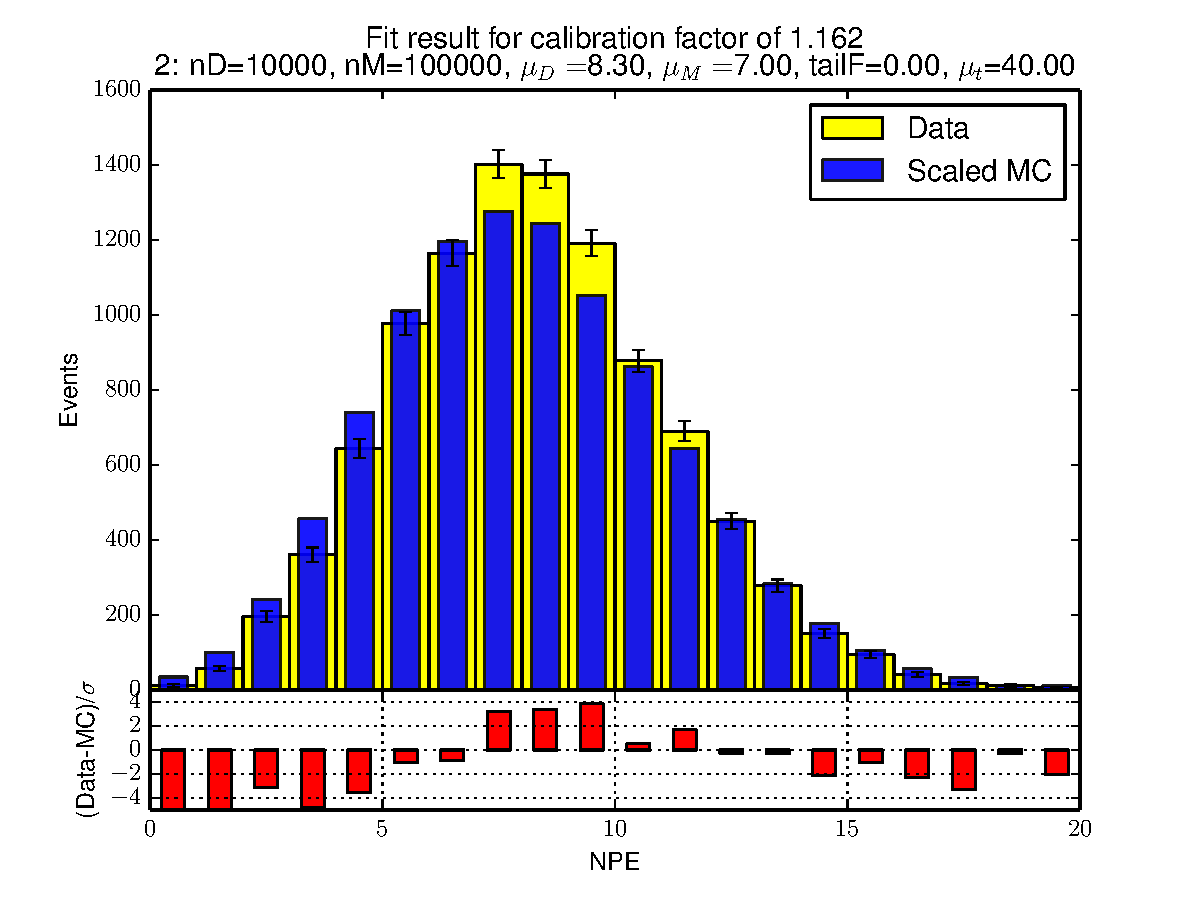
\includegraphics[width=0.45\textwidth]{../FIGURES/02/FIG_Fit_result_for_calibration_factor_of_1_162.pdf} 
\caption{Data compared to nominal MC, MC scaled by the best fit calibration factor, scans of $\chi^2$ over a large range and about the minimum for configuration 02. Data compared to MC scaled by two randomly chosen calibration factors.} 
\label{tab:best_02} 
\end{center} \end{figure} 

 \begin{figure}[htbp] \begin{center} 
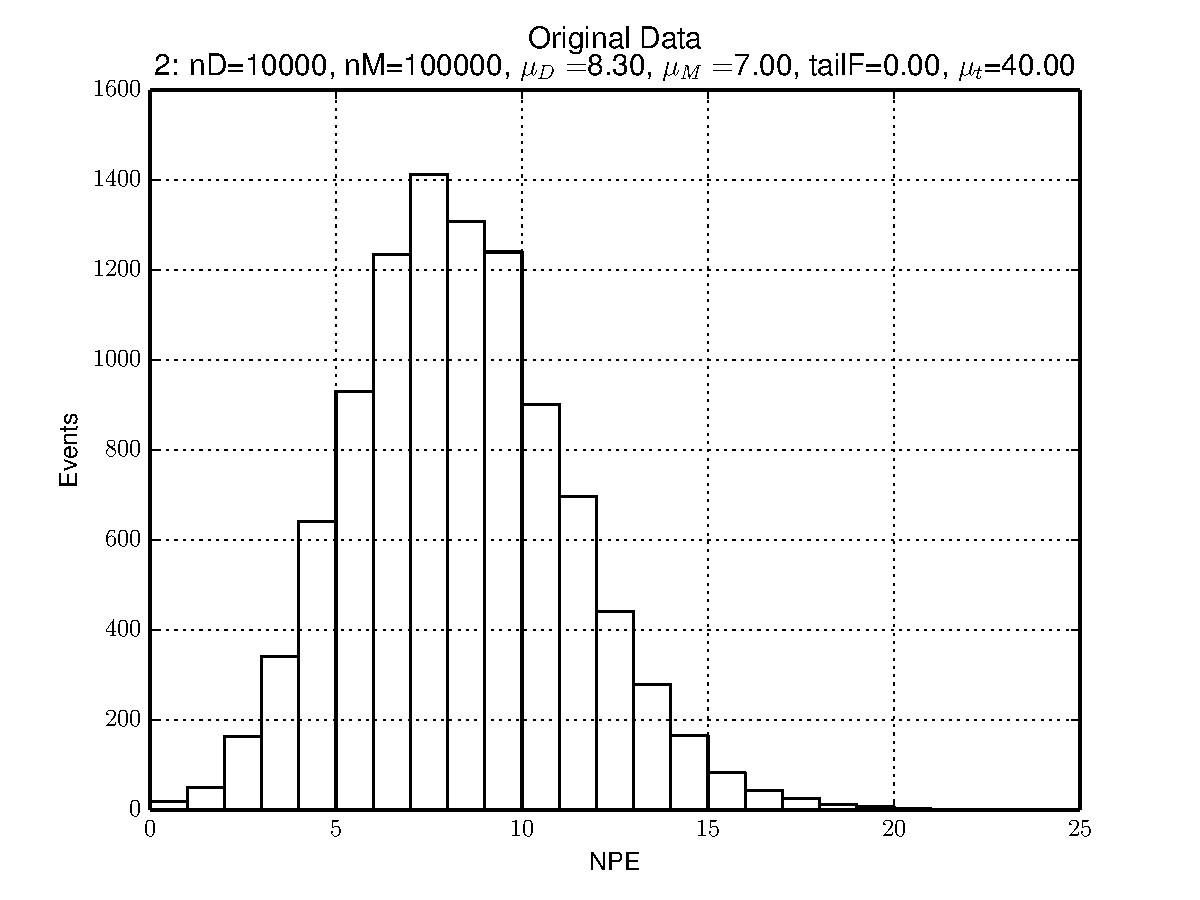
\includegraphics[width=0.45\textwidth]{../FIGURES/02/FIG_Original_Data.pdf} 
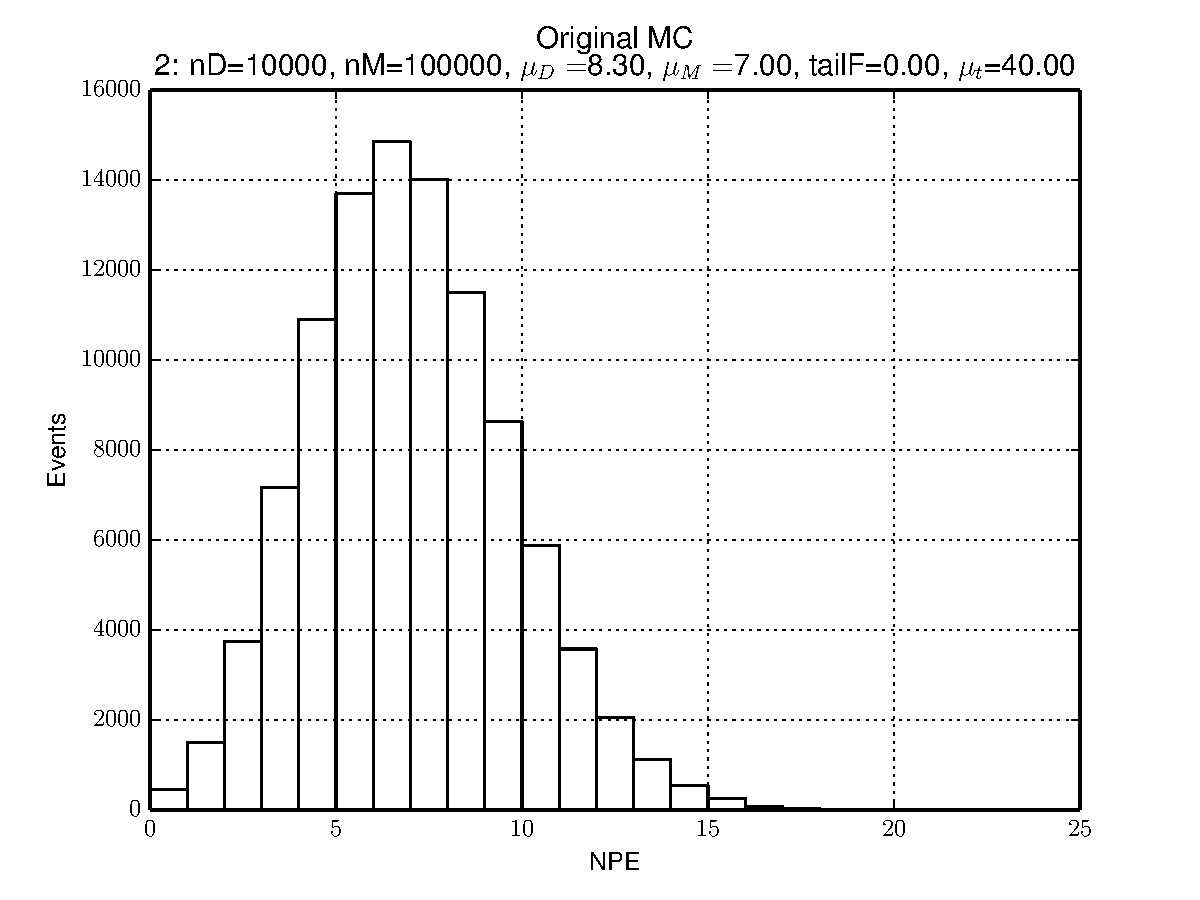
\includegraphics[width=0.45\textwidth]{../FIGURES/02/FIG_Original_MC.pdf} 
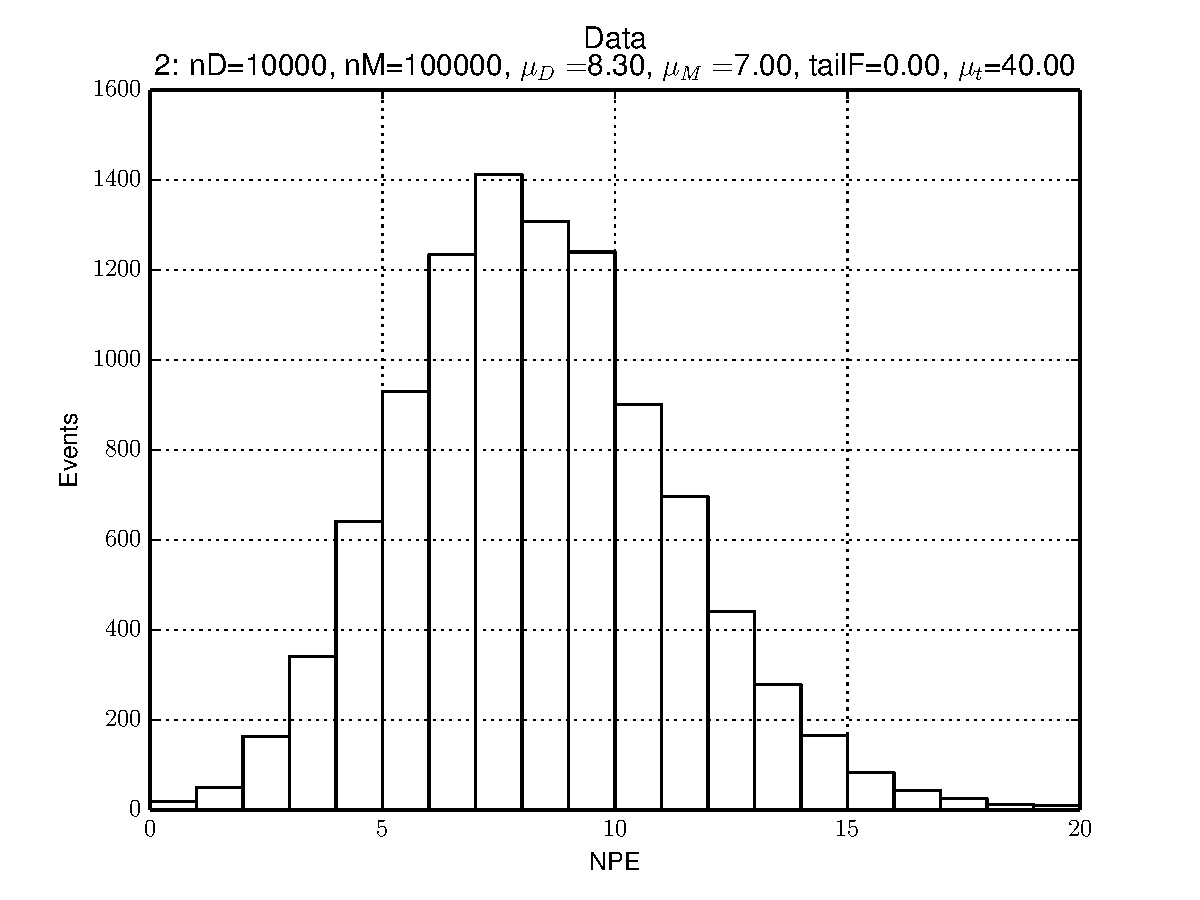
\includegraphics[width=0.45\textwidth]{../FIGURES/02/FIG_Data.pdf} 
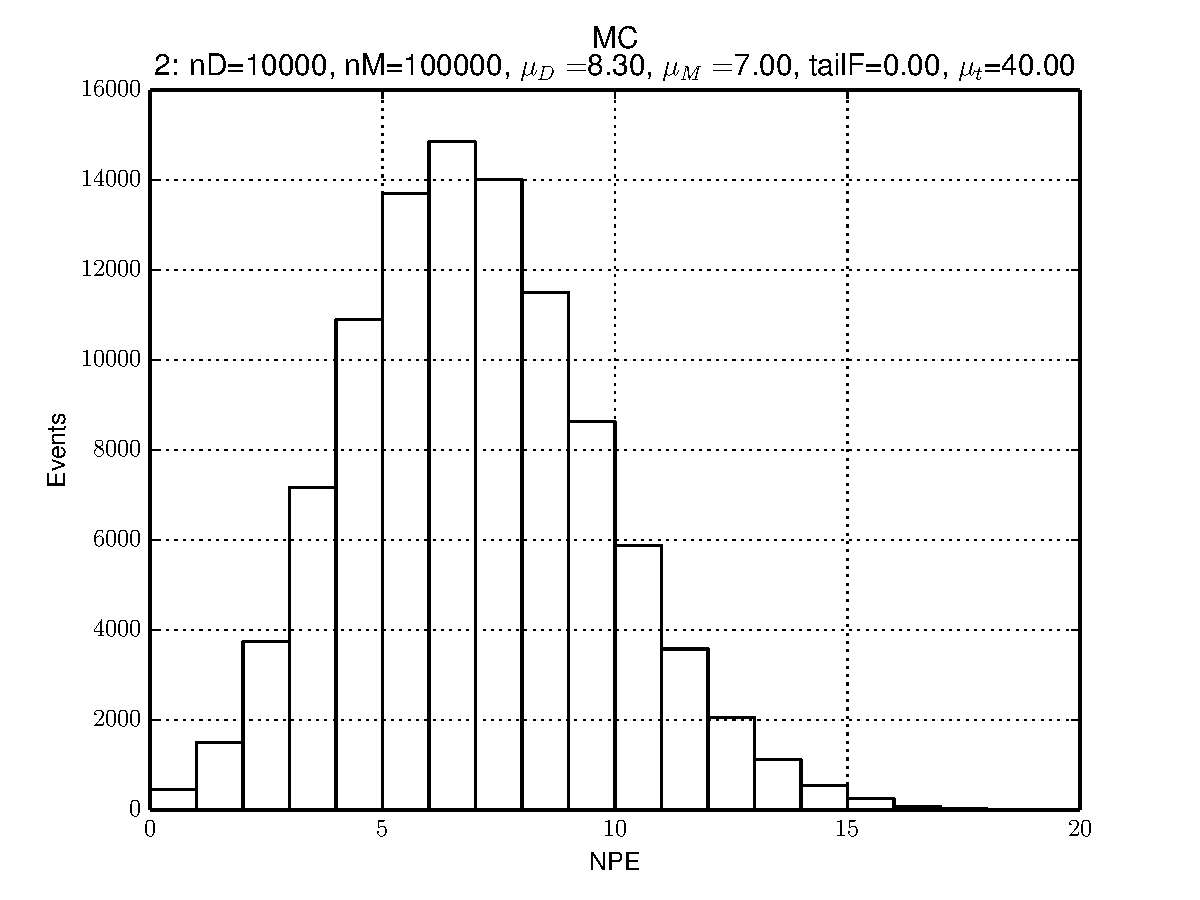
\includegraphics[width=0.45\textwidth]{../FIGURES/02/FIG_MC.pdf} 
\caption{NPE histograms for data and MC for configuration 02. Top are original hists. Bottom are hists after truncation at bin containing less than 10 entries with that bin containing overflows.} 
\label{tab:npe_02} 
\end{center} \end{figure} 

  \clearpage

 \begin{figure}[htbp] \begin{center} 
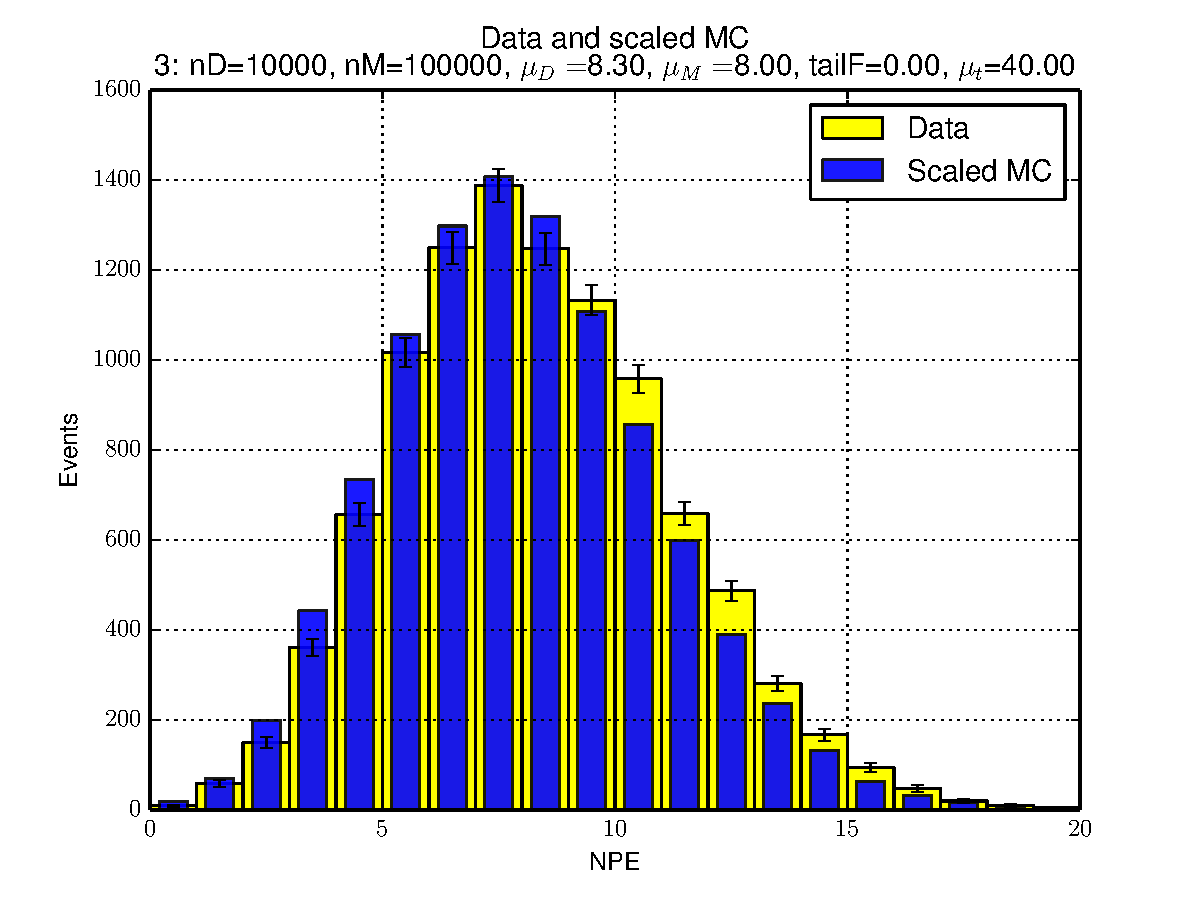
\includegraphics[width=0.45\textwidth]{../FIGURES/03/FIG_Data_and_scaled_MC.pdf} 
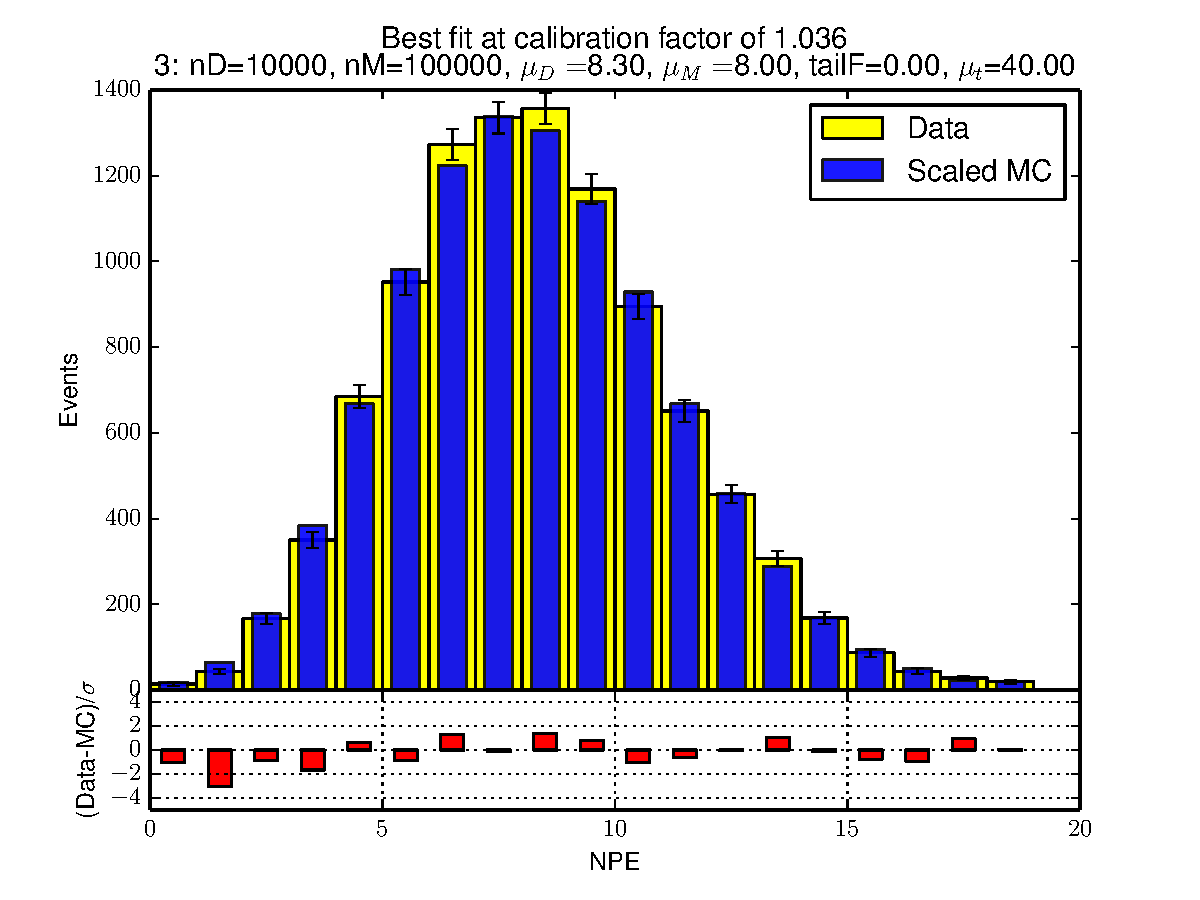
\includegraphics[width=0.45\textwidth]{../FIGURES/03/FIG_Best_fit_at_calibration_factor_of_1_036.pdf} 
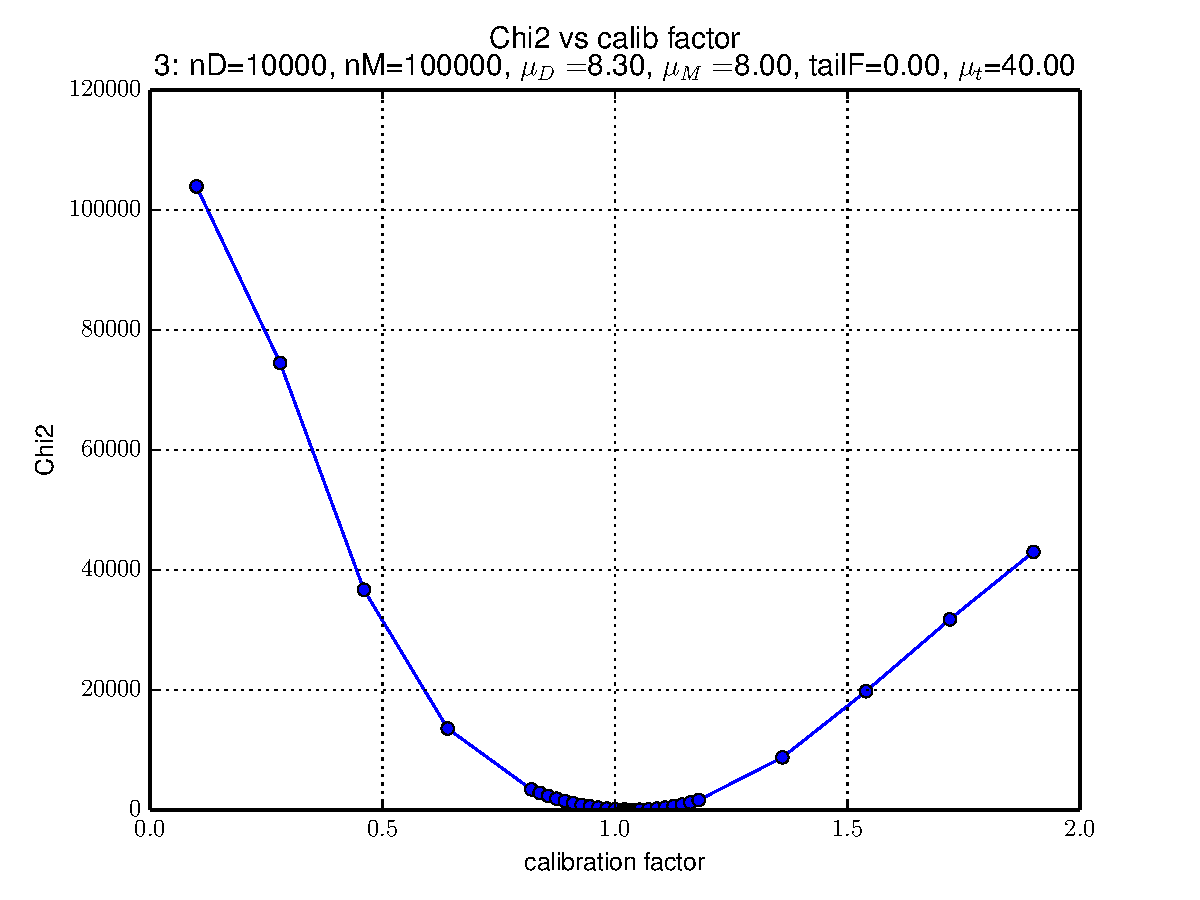
\includegraphics[width=0.45\textwidth]{../FIGURES/03/FIG_Chi2_vs_calib_factor.pdf} 
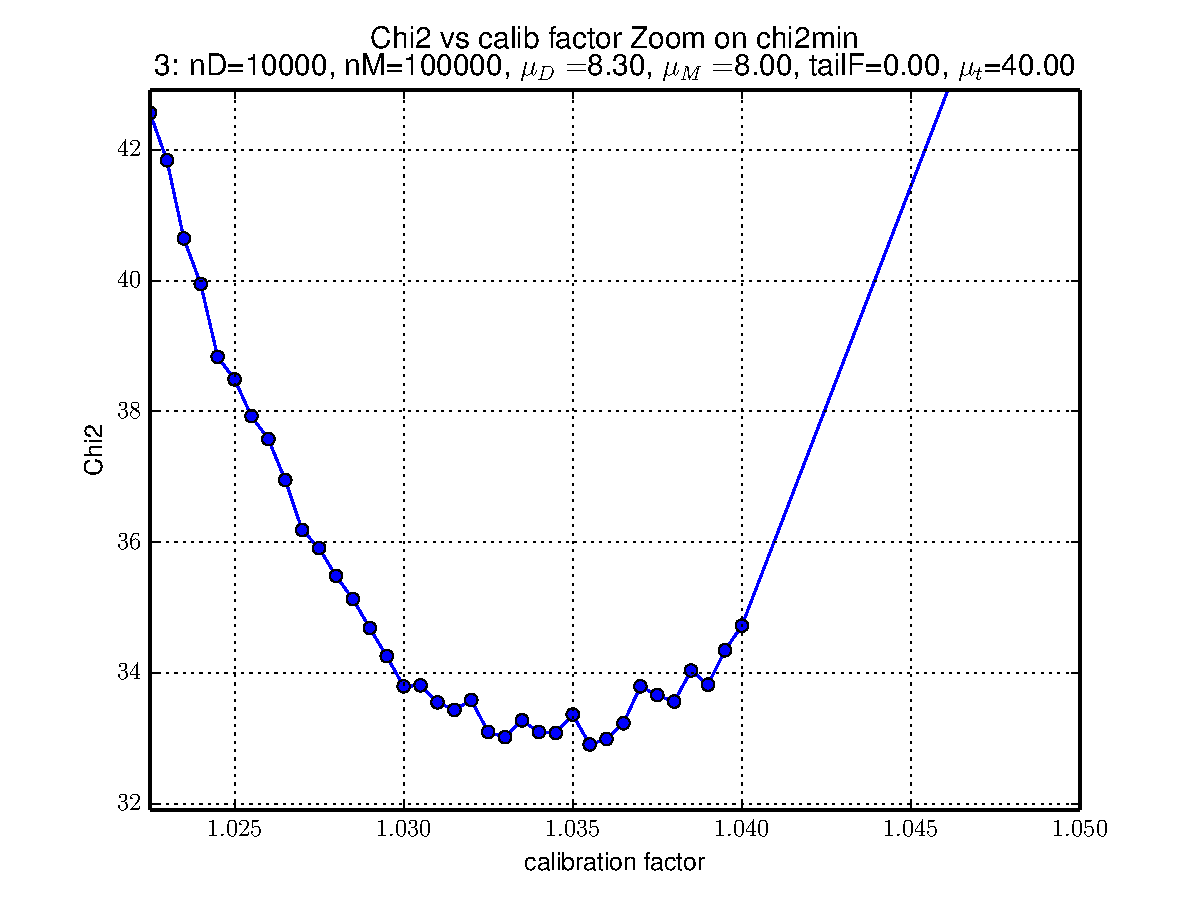
\includegraphics[width=0.45\textwidth]{../FIGURES/03/FIG_Chi2_vs_calib_factor_Zoom_on_chi2min.pdf} 
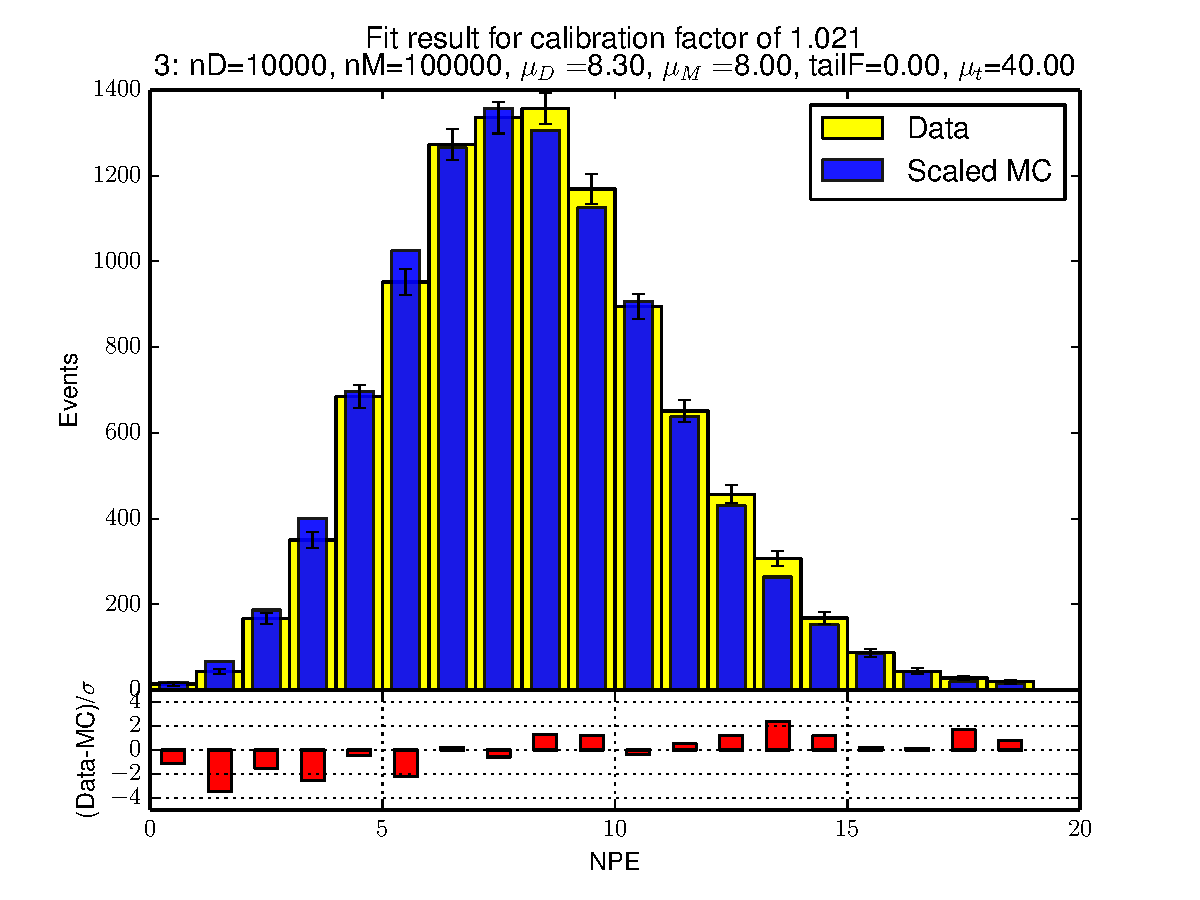
\includegraphics[width=0.45\textwidth]{../FIGURES/03/FIG_Fit_result_for_calibration_factor_of_1_021.pdf} 
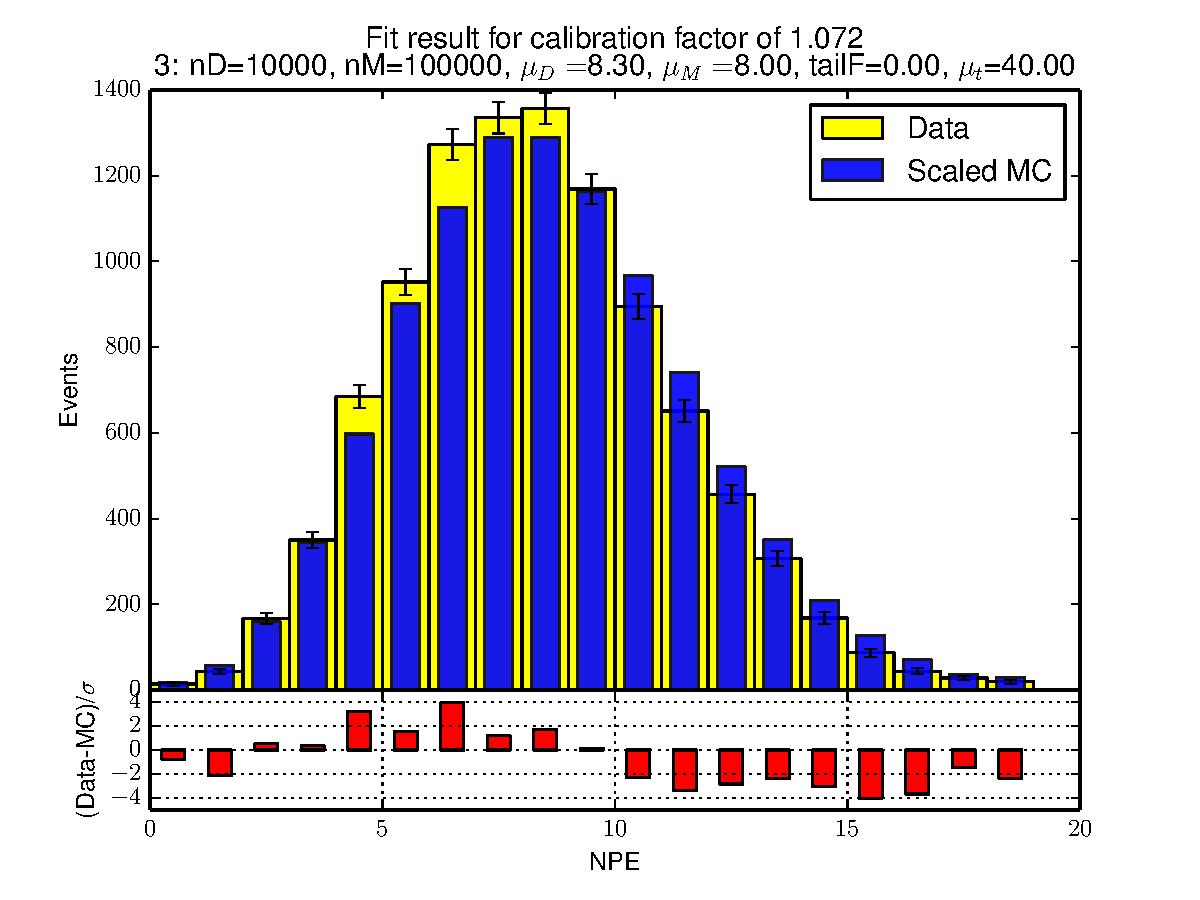
\includegraphics[width=0.45\textwidth]{../FIGURES/03/FIG_Fit_result_for_calibration_factor_of_1_072.pdf} 
\caption{Data compared to nominal MC, MC scaled by the best fit calibration factor, scans of $\chi^2$ over a large range and about the minimum for configuration 03. Data compared to MC scaled by two randomly chosen calibration factors.} 
\label{tab:best_03} 
\end{center} \end{figure} 

 \begin{figure}[htbp] \begin{center} 
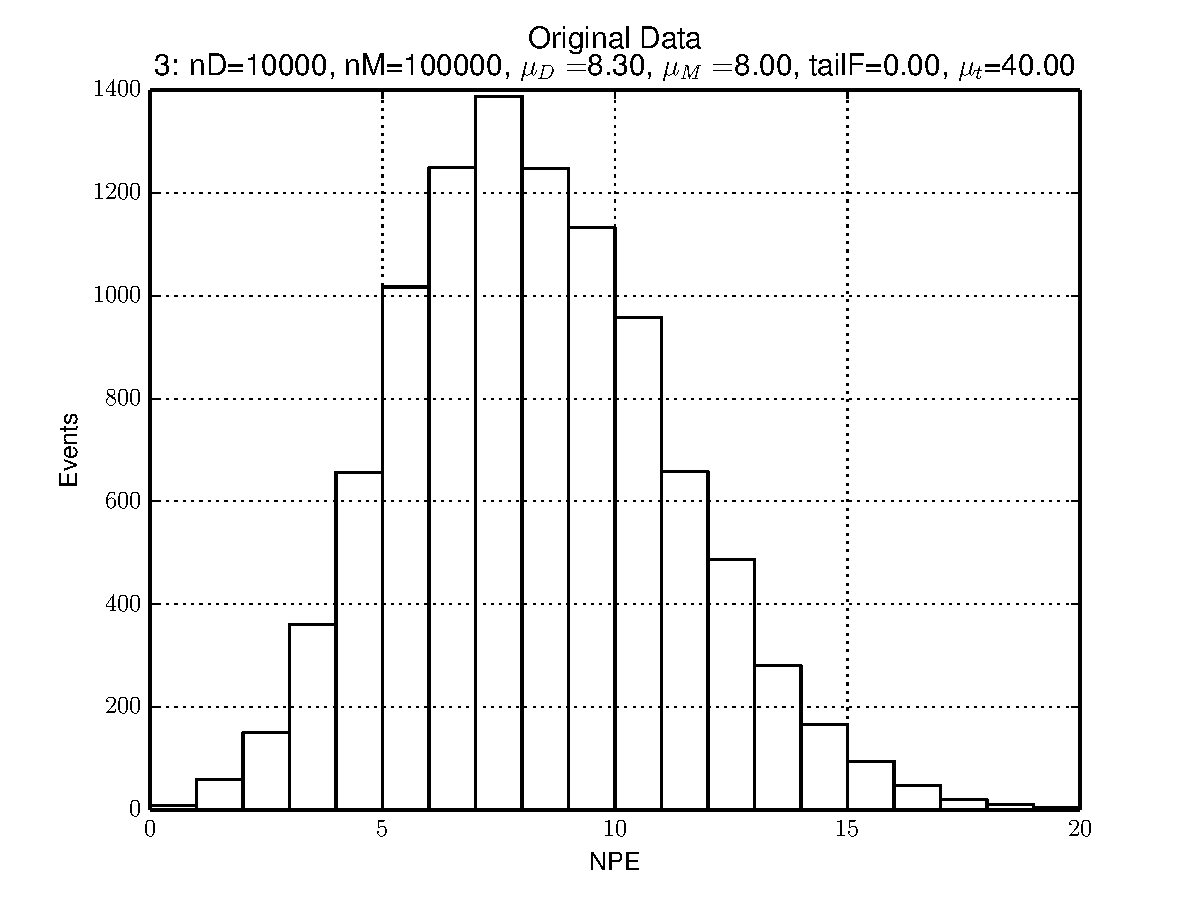
\includegraphics[width=0.45\textwidth]{../FIGURES/03/FIG_Original_Data.pdf} 
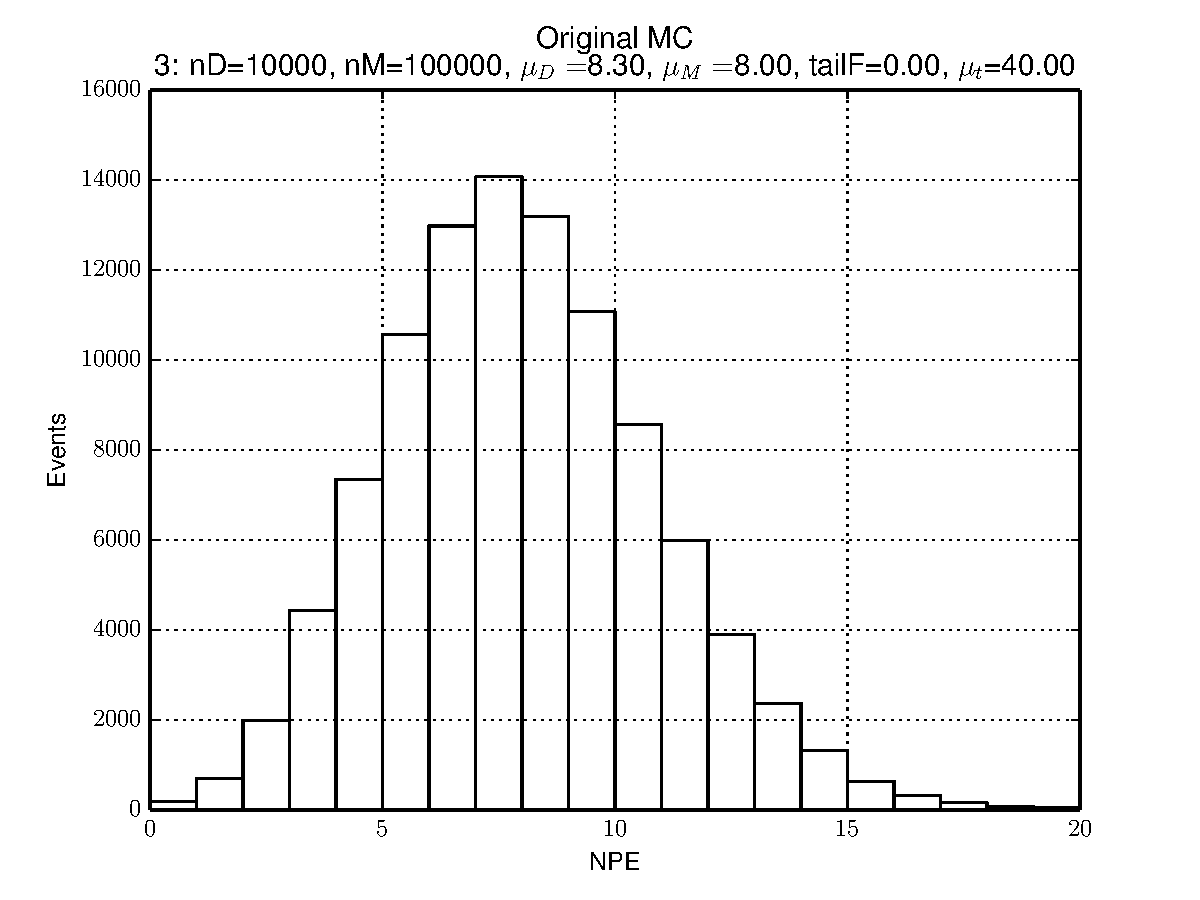
\includegraphics[width=0.45\textwidth]{../FIGURES/03/FIG_Original_MC.pdf} 
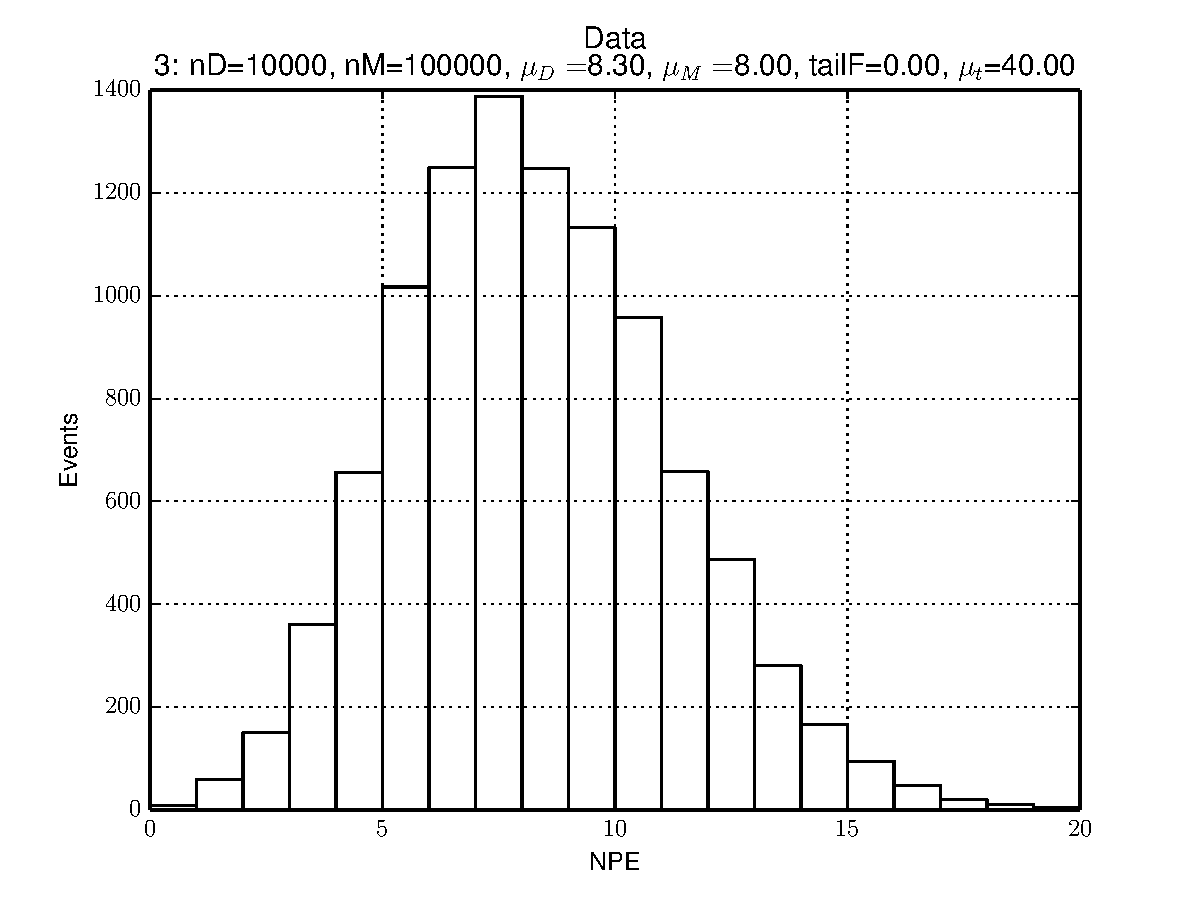
\includegraphics[width=0.45\textwidth]{../FIGURES/03/FIG_Data.pdf} 
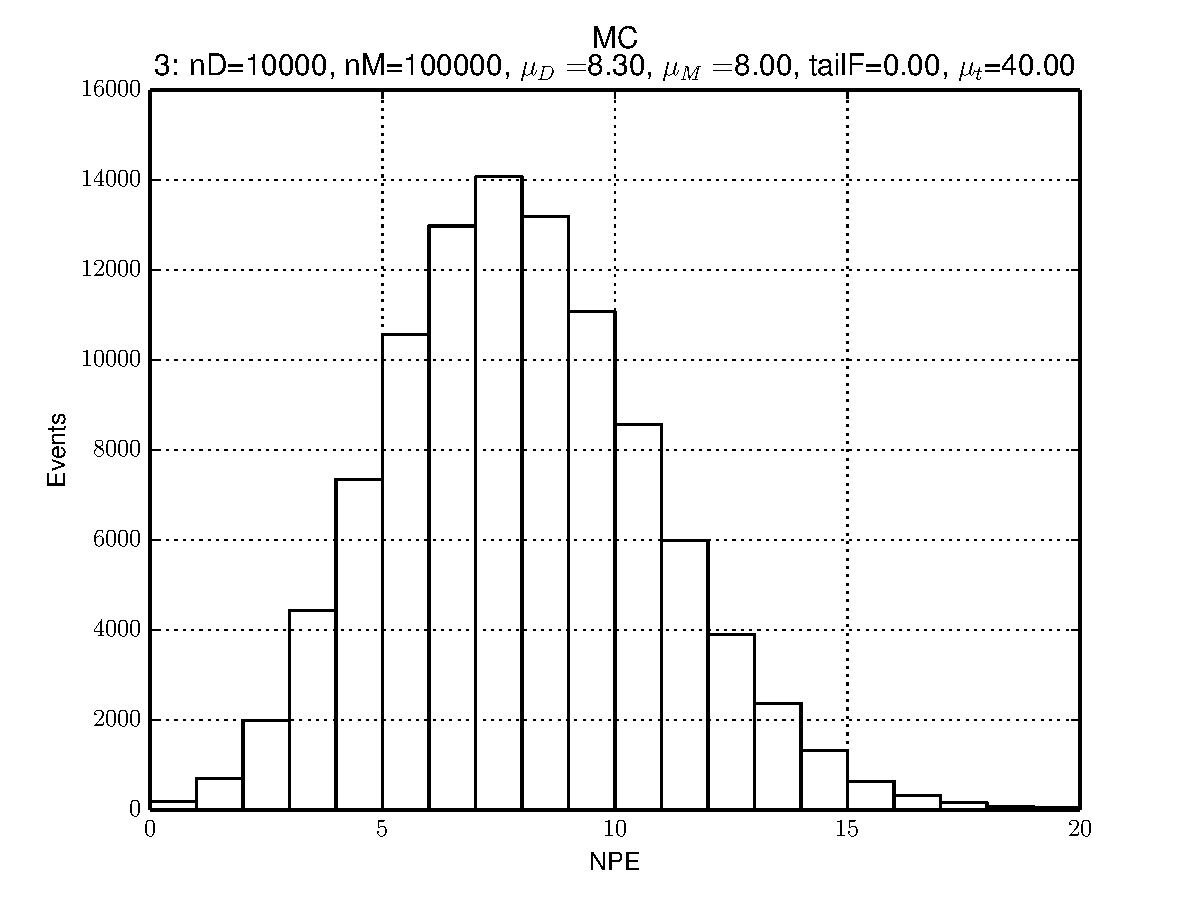
\includegraphics[width=0.45\textwidth]{../FIGURES/03/FIG_MC.pdf} 
\caption{NPE histograms for data and MC for configuration 03. Top are original hists. Bottom are hists after truncation at bin containing less than 10 entries with that bin containing overflows.} 
\label{tab:npe_03} 
\end{center} \end{figure} 

  \clearpage

 \begin{figure}[htbp] \begin{center} 
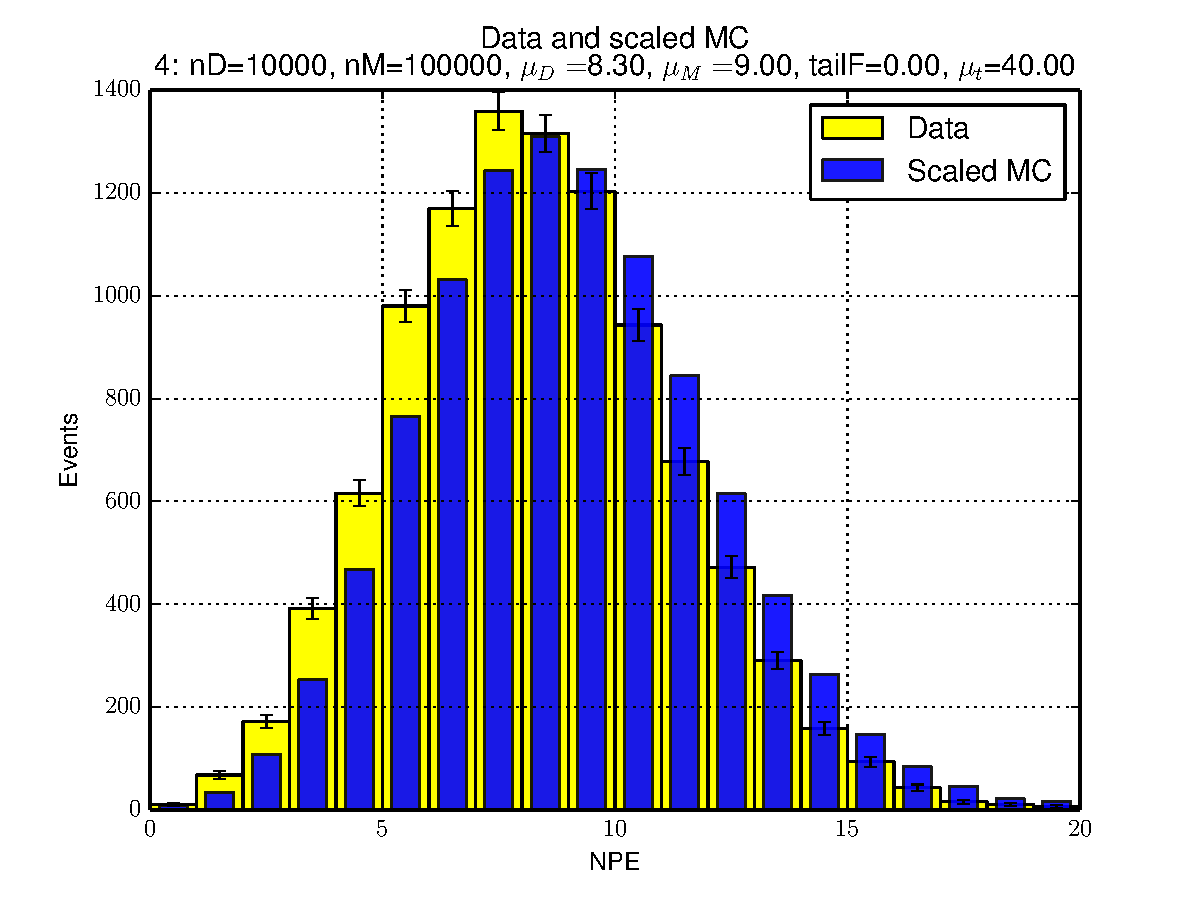
\includegraphics[width=0.45\textwidth]{../FIGURES/04/FIG_Data_and_scaled_MC.pdf} 
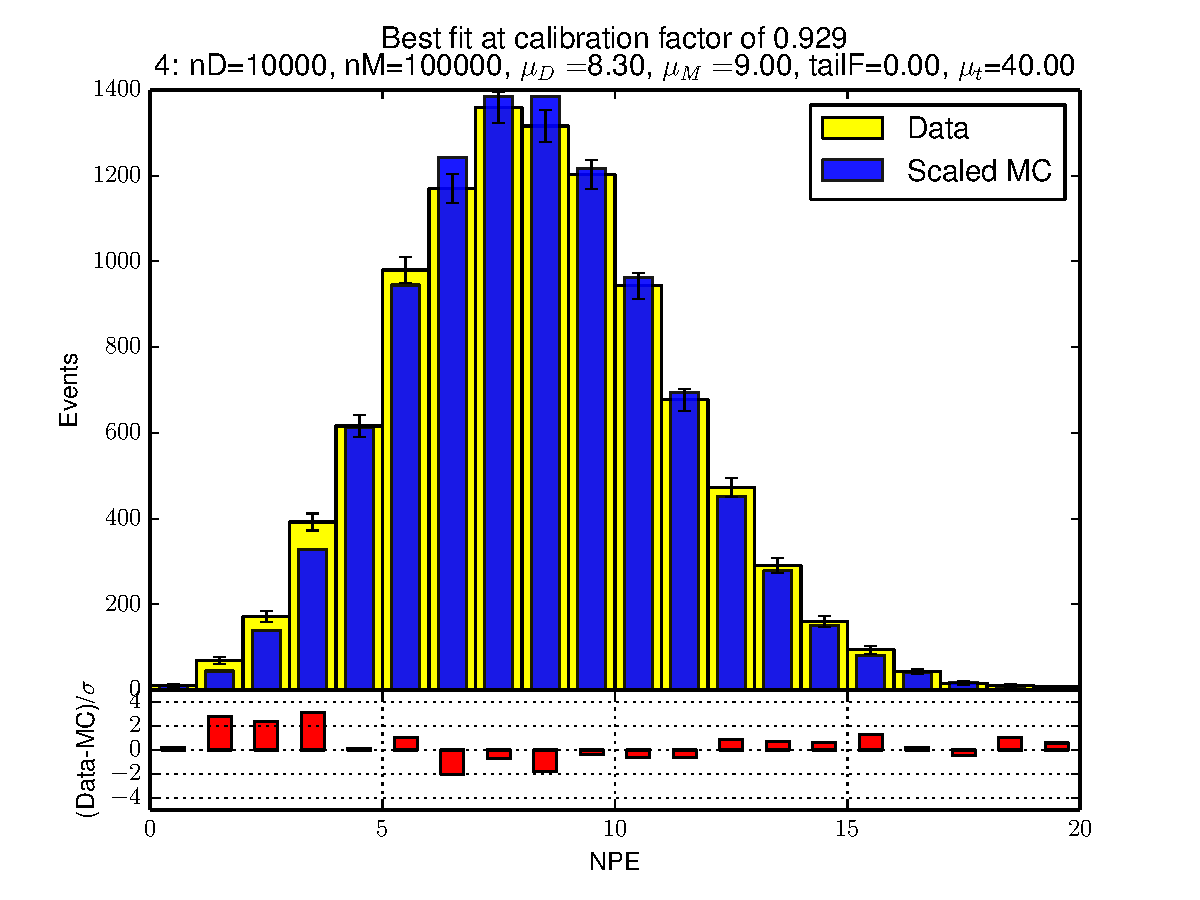
\includegraphics[width=0.45\textwidth]{../FIGURES/04/FIG_Best_fit_at_calibration_factor_of_0_929.pdf} 
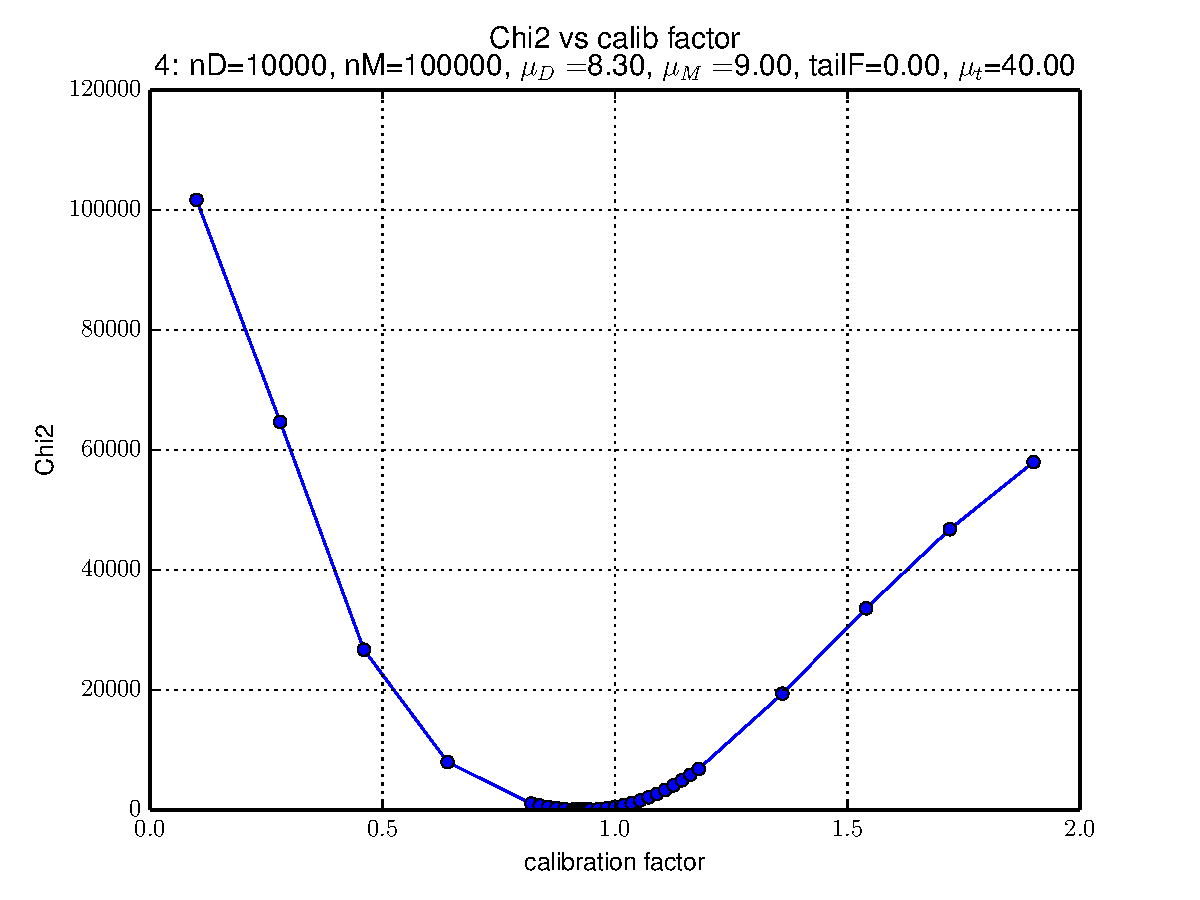
\includegraphics[width=0.45\textwidth]{../FIGURES/04/FIG_Chi2_vs_calib_factor.pdf} 
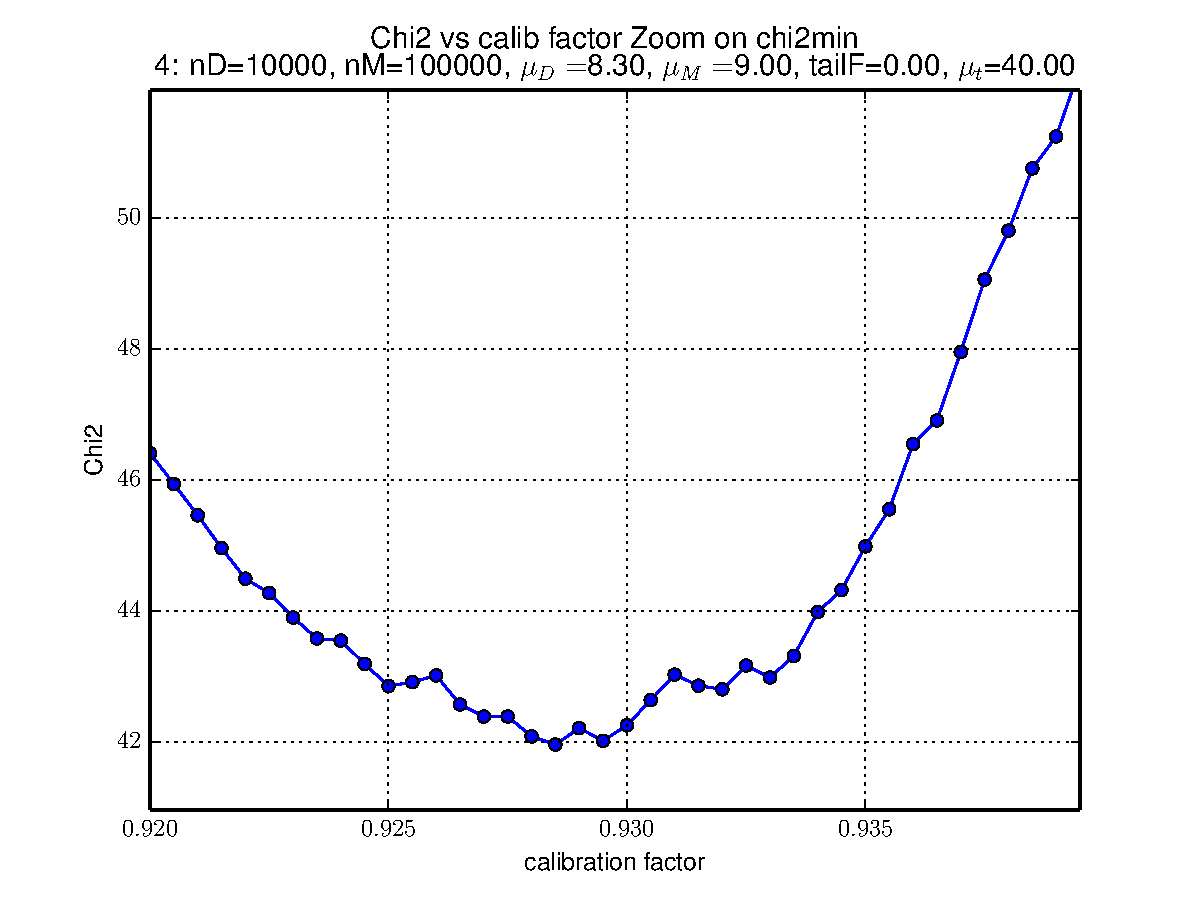
\includegraphics[width=0.45\textwidth]{../FIGURES/04/FIG_Chi2_vs_calib_factor_Zoom_on_chi2min.pdf} 
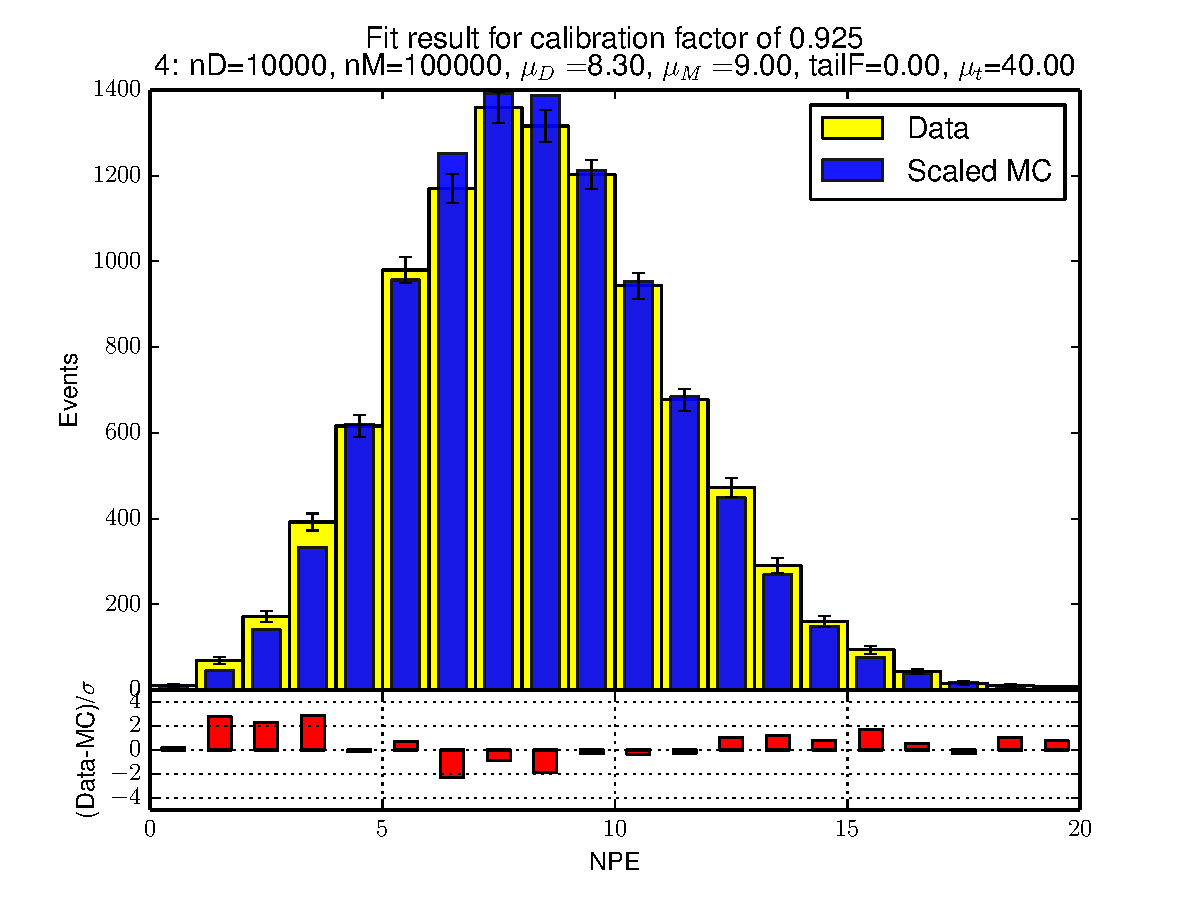
\includegraphics[width=0.45\textwidth]{../FIGURES/04/FIG_Fit_result_for_calibration_factor_of_0_925.pdf} 
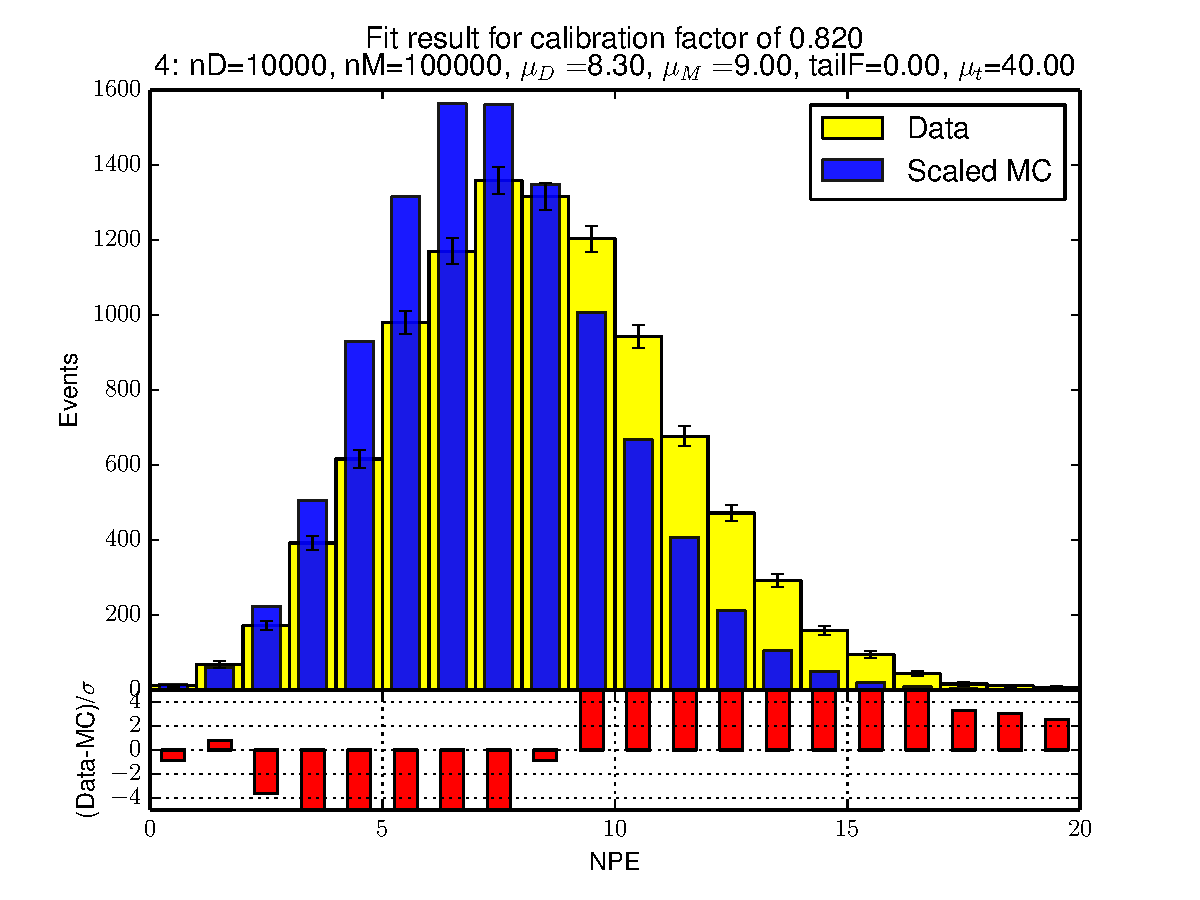
\includegraphics[width=0.45\textwidth]{../FIGURES/04/FIG_Fit_result_for_calibration_factor_of_0_820.pdf} 
\caption{Data compared to nominal MC, MC scaled by the best fit calibration factor, scans of $\chi^2$ over a large range and about the minimum for configuration 04. Data compared to MC scaled by two randomly chosen calibration factors.} 
\label{tab:best_04} 
\end{center} \end{figure} 

 \begin{figure}[htbp] \begin{center} 
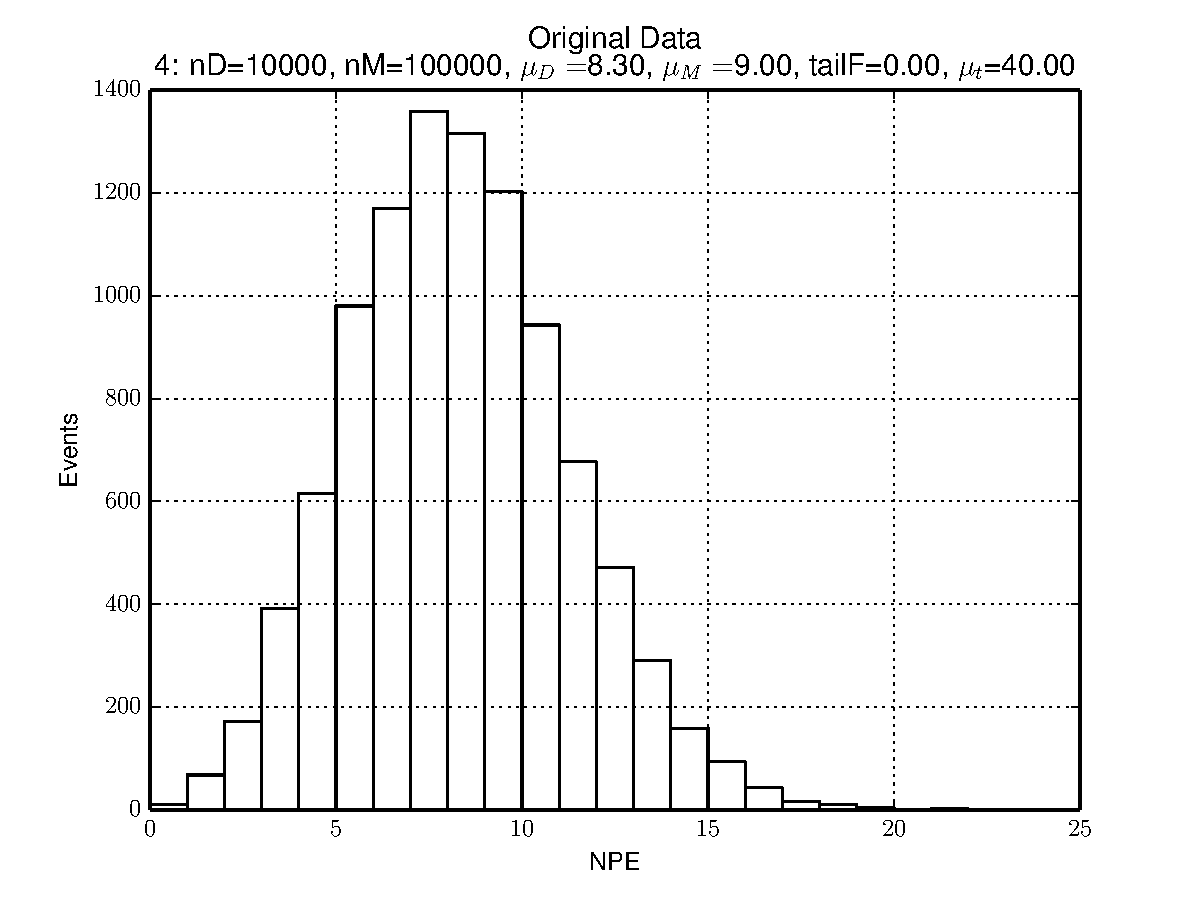
\includegraphics[width=0.45\textwidth]{../FIGURES/04/FIG_Original_Data.pdf} 
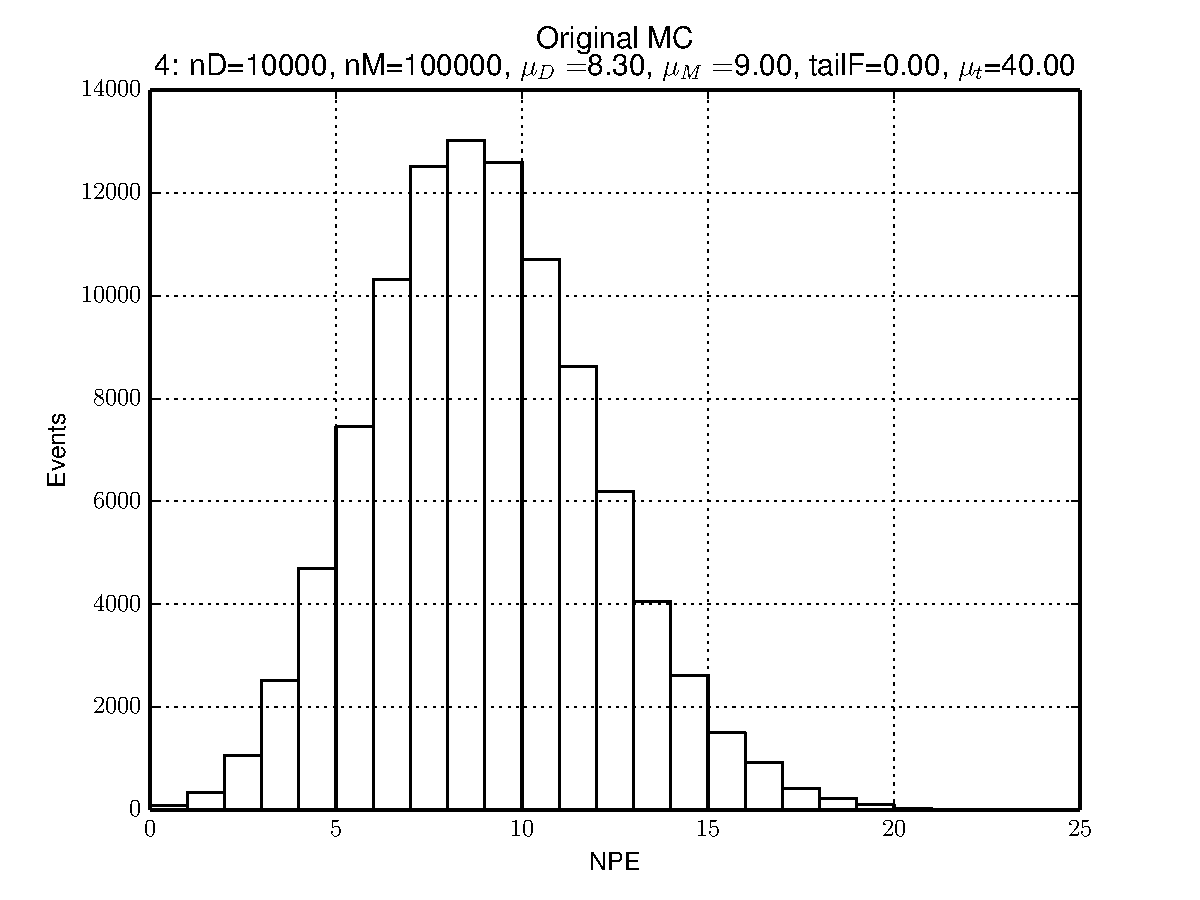
\includegraphics[width=0.45\textwidth]{../FIGURES/04/FIG_Original_MC.pdf} 
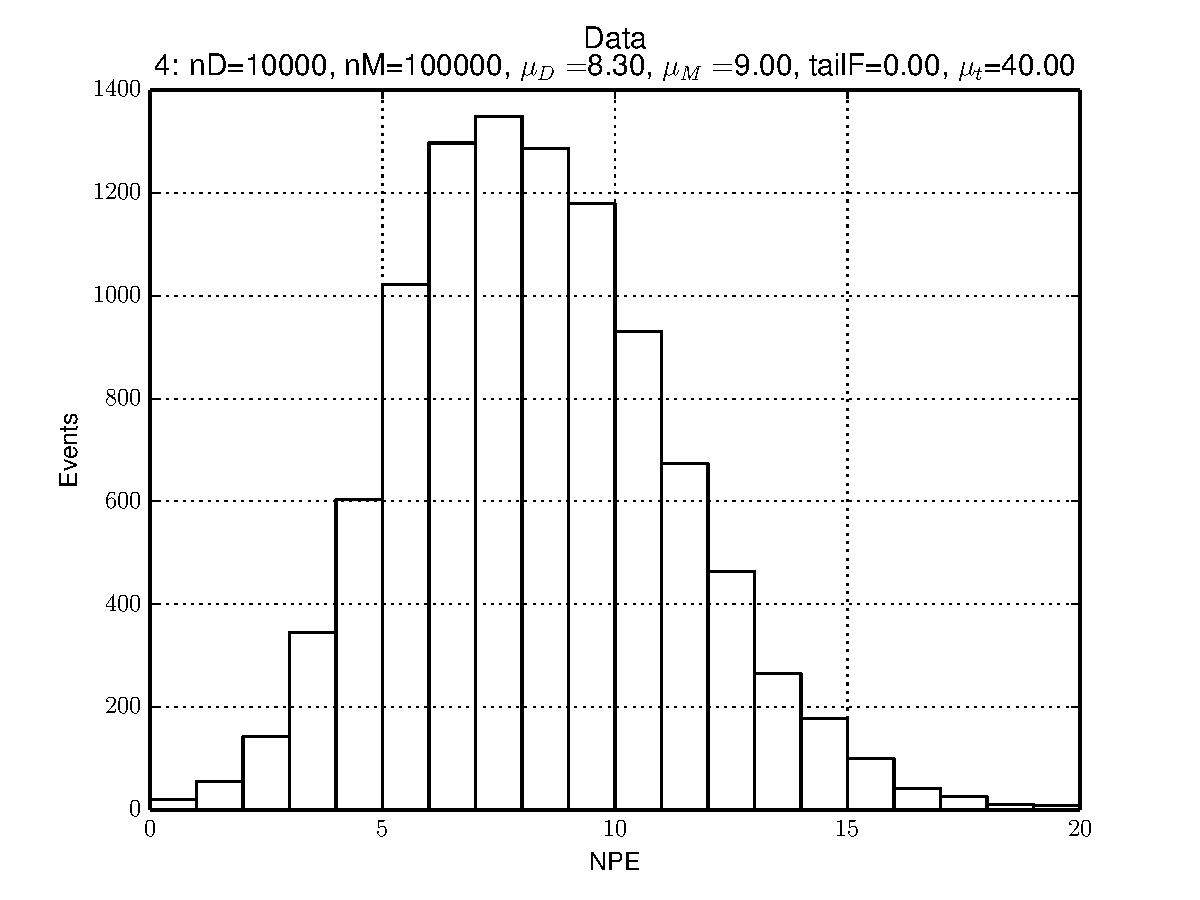
\includegraphics[width=0.45\textwidth]{../FIGURES/04/FIG_Data.pdf} 
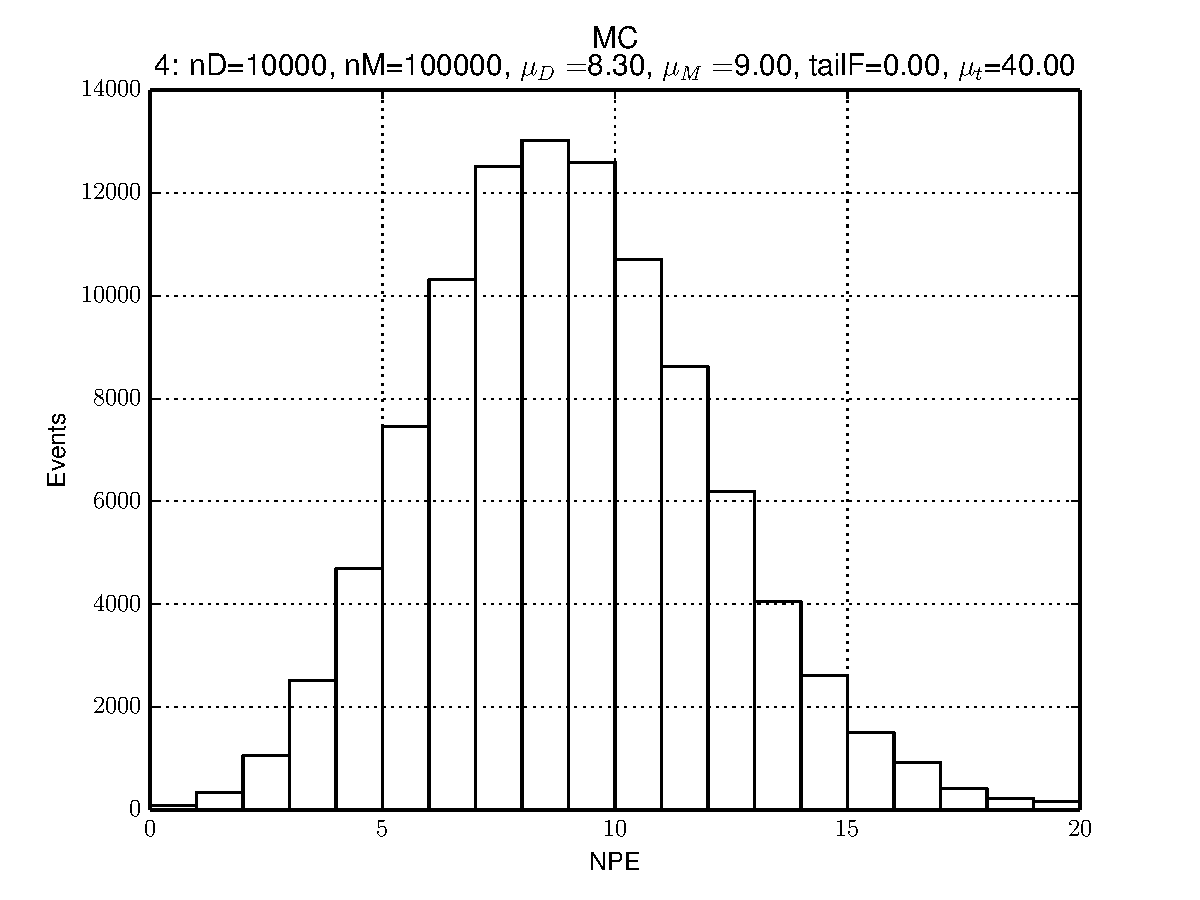
\includegraphics[width=0.45\textwidth]{../FIGURES/04/FIG_MC.pdf} 
\caption{NPE histograms for data and MC for configuration 04. Top are original hists. Bottom are hists after truncation at bin containing less than 10 entries with that bin containing overflows.} 
\label{tab:npe_04} 
\end{center} \end{figure} 

  \clearpage

 \begin{figure}[htbp] \begin{center} 
\includegraphics[width=0.45\textwidth]{../FIGURES/05/FIG_Data_and_scaled_MC.pdf} 
\includegraphics[width=0.45\textwidth]{../FIGURES/05/FIG_Best_fit_at_calibration_factor_of_0_840.pdf} 
\includegraphics[width=0.45\textwidth]{../FIGURES/05/FIG_Chi2_vs_calib_factor.pdf} 
\includegraphics[width=0.45\textwidth]{../FIGURES/05/FIG_Chi2_vs_calib_factor_Zoom_on_chi2min.pdf} 
\includegraphics[width=0.45\textwidth]{../FIGURES/05/FIG_Fit_result_for_calibration_factor_of_1_900.pdf} 
\includegraphics[width=0.45\textwidth]{../FIGURES/05/FIG_Fit_result_for_calibration_factor_of_0_766.pdf} 
\caption{Data compared to nominal MC, MC scaled by the best fit calibration factor, scans of $\chi^2$ over a large range and about the minimum for configuration 05. Data compared to MC scaled by two randomly chosen calibration factors.} 
\label{tab:best_05} 
\end{center} \end{figure} 

 \begin{figure}[htbp] \begin{center} 
\includegraphics[width=0.45\textwidth]{../FIGURES/05/FIG_Original_Data.pdf} 
\includegraphics[width=0.45\textwidth]{../FIGURES/05/FIG_Original_MC.pdf} 
\includegraphics[width=0.45\textwidth]{../FIGURES/05/FIG_Data.pdf} 
\includegraphics[width=0.45\textwidth]{../FIGURES/05/FIG_MC.pdf} 
\caption{NPE histograms for data and MC for configuration 05. Top are original hists. Bottom are hists after truncation at bin containing less than 10 entries with that bin containing overflows.} 
\label{tab:npe_05} 
\end{center} \end{figure} 

  \clearpage

 \begin{figure}[htbp] \begin{center} 
\includegraphics[width=0.45\textwidth]{../FIGURES/06/FIG_Data_and_scaled_MC.pdf} 
\includegraphics[width=0.45\textwidth]{../FIGURES/06/FIG_Best_fit_at_calibration_factor_of_1_365.pdf} 
\includegraphics[width=0.45\textwidth]{../FIGURES/06/FIG_Chi2_vs_calib_factor.pdf} 
\includegraphics[width=0.45\textwidth]{../FIGURES/06/FIG_Chi2_vs_calib_factor_Zoom_on_chi2min.pdf} 
\includegraphics[width=0.45\textwidth]{../FIGURES/06/FIG_Fit_result_for_calibration_factor_of_1_180.pdf} 
\includegraphics[width=0.45\textwidth]{../FIGURES/06/FIG_Fit_result_for_calibration_factor_of_1_357.pdf} 
\caption{Data compared to nominal MC, MC scaled by the best fit calibration factor, scans of $\chi^2$ over a large range and about the minimum for configuration 06. Data compared to MC scaled by two randomly chosen calibration factors.} 
\label{tab:best_06} 
\end{center} \end{figure} 

 \begin{figure}[htbp] \begin{center} 
\includegraphics[width=0.45\textwidth]{../FIGURES/06/FIG_Original_Data.pdf} 
\includegraphics[width=0.45\textwidth]{../FIGURES/06/FIG_Original_MC.pdf} 
\includegraphics[width=0.45\textwidth]{../FIGURES/06/FIG_Data.pdf} 
\includegraphics[width=0.45\textwidth]{../FIGURES/06/FIG_MC.pdf} 
\caption{NPE histograms for data and MC for configuration 06. Top are original hists. Bottom are hists after truncation at bin containing less than 10 entries with that bin containing overflows.} 
\label{tab:npe_06} 
\end{center} \end{figure} 

  \clearpage

 \begin{figure}[htbp] \begin{center} 
\includegraphics[width=0.45\textwidth]{../FIGURES/07/FIG_Data_and_scaled_MC.pdf} 
\includegraphics[width=0.45\textwidth]{../FIGURES/07/FIG_Best_fit_at_calibration_factor_of_1_180.pdf} 
\includegraphics[width=0.45\textwidth]{../FIGURES/07/FIG_Chi2_vs_calib_factor.pdf} 
\includegraphics[width=0.45\textwidth]{../FIGURES/07/FIG_Chi2_vs_calib_factor_Zoom_on_chi2min.pdf} 
\includegraphics[width=0.45\textwidth]{../FIGURES/07/FIG_Fit_result_for_calibration_factor_of_1_176.pdf} 
\includegraphics[width=0.45\textwidth]{../FIGURES/07/FIG_Fit_result_for_calibration_factor_of_1_166.pdf} 
\caption{Data compared to nominal MC, MC scaled by the best fit calibration factor, scans of $\chi^2$ over a large range and about the minimum for configuration 07. Data compared to MC scaled by two randomly chosen calibration factors.} 
\label{tab:best_07} 
\end{center} \end{figure} 

 \begin{figure}[htbp] \begin{center} 
\includegraphics[width=0.45\textwidth]{../FIGURES/07/FIG_Original_Data.pdf} 
\includegraphics[width=0.45\textwidth]{../FIGURES/07/FIG_Original_MC.pdf} 
\includegraphics[width=0.45\textwidth]{../FIGURES/07/FIG_Data.pdf} 
\includegraphics[width=0.45\textwidth]{../FIGURES/07/FIG_MC.pdf} 
\caption{NPE histograms for data and MC for configuration 07. Top are original hists. Bottom are hists after truncation at bin containing less than 10 entries with that bin containing overflows.} 
\label{tab:npe_07} 
\end{center} \end{figure} 

  \clearpage

 \begin{figure}[htbp] \begin{center} 
\includegraphics[width=0.45\textwidth]{../FIGURES/08/FIG_Data_and_scaled_MC.pdf} 
\includegraphics[width=0.45\textwidth]{../FIGURES/08/FIG_Best_fit_at_calibration_factor_of_1_042.pdf} 
\includegraphics[width=0.45\textwidth]{../FIGURES/08/FIG_Chi2_vs_calib_factor.pdf} 
\includegraphics[width=0.45\textwidth]{../FIGURES/08/FIG_Chi2_vs_calib_factor_Zoom_on_chi2min.pdf} 
\includegraphics[width=0.45\textwidth]{../FIGURES/08/FIG_Fit_result_for_calibration_factor_of_0_964.pdf} 
\includegraphics[width=0.45\textwidth]{../FIGURES/08/FIG_Fit_result_for_calibration_factor_of_0_856.pdf} 
\caption{Data compared to nominal MC, MC scaled by the best fit calibration factor, scans of $\chi^2$ over a large range and about the minimum for configuration 08. Data compared to MC scaled by two randomly chosen calibration factors.} 
\label{tab:best_08} 
\end{center} \end{figure} 

 \begin{figure}[htbp] \begin{center} 
\includegraphics[width=0.45\textwidth]{../FIGURES/08/FIG_Original_Data.pdf} 
\includegraphics[width=0.45\textwidth]{../FIGURES/08/FIG_Original_MC.pdf} 
\includegraphics[width=0.45\textwidth]{../FIGURES/08/FIG_Data.pdf} 
\includegraphics[width=0.45\textwidth]{../FIGURES/08/FIG_MC.pdf} 
\caption{NPE histograms for data and MC for configuration 08. Top are original hists. Bottom are hists after truncation at bin containing less than 10 entries with that bin containing overflows.} 
\label{tab:npe_08} 
\end{center} \end{figure} 

  \clearpage

 \begin{figure}[htbp] \begin{center} 
\includegraphics[width=0.45\textwidth]{../FIGURES/09/FIG_Data_and_scaled_MC.pdf} 
\includegraphics[width=0.45\textwidth]{../FIGURES/09/FIG_Best_fit_at_calibration_factor_of_0_928.pdf} 
\includegraphics[width=0.45\textwidth]{../FIGURES/09/FIG_Chi2_vs_calib_factor.pdf} 
\includegraphics[width=0.45\textwidth]{../FIGURES/09/FIG_Chi2_vs_calib_factor_Zoom_on_chi2min.pdf} 
\includegraphics[width=0.45\textwidth]{../FIGURES/09/FIG_Fit_result_for_calibration_factor_of_1_900.pdf} 
\includegraphics[width=0.45\textwidth]{../FIGURES/09/FIG_Fit_result_for_calibration_factor_of_0_941.pdf} 
\caption{Data compared to nominal MC, MC scaled by the best fit calibration factor, scans of $\chi^2$ over a large range and about the minimum for configuration 09. Data compared to MC scaled by two randomly chosen calibration factors.} 
\label{tab:best_09} 
\end{center} \end{figure} 

 \begin{figure}[htbp] \begin{center} 
\includegraphics[width=0.45\textwidth]{../FIGURES/09/FIG_Original_Data.pdf} 
\includegraphics[width=0.45\textwidth]{../FIGURES/09/FIG_Original_MC.pdf} 
\includegraphics[width=0.45\textwidth]{../FIGURES/09/FIG_Data.pdf} 
\includegraphics[width=0.45\textwidth]{../FIGURES/09/FIG_MC.pdf} 
\caption{NPE histograms for data and MC for configuration 09. Top are original hists. Bottom are hists after truncation at bin containing less than 10 entries with that bin containing overflows.} 
\label{tab:npe_09} 
\end{center} \end{figure} 

  \clearpage

 \begin{figure}[htbp] \begin{center} 
\includegraphics[width=0.45\textwidth]{../FIGURES/10/FIG_Data_and_scaled_MC.pdf} 
\includegraphics[width=0.45\textwidth]{../FIGURES/10/FIG_Best_fit_at_calibration_factor_of_0_841.pdf} 
\includegraphics[width=0.45\textwidth]{../FIGURES/10/FIG_Chi2_vs_calib_factor.pdf} 
\includegraphics[width=0.45\textwidth]{../FIGURES/10/FIG_Chi2_vs_calib_factor_Zoom_on_chi2min.pdf} 
\includegraphics[width=0.45\textwidth]{../FIGURES/10/FIG_Fit_result_for_calibration_factor_of_0_847.pdf} 
\includegraphics[width=0.45\textwidth]{../FIGURES/10/FIG_Fit_result_for_calibration_factor_of_0_837.pdf} 
\caption{Data compared to nominal MC, MC scaled by the best fit calibration factor, scans of $\chi^2$ over a large range and about the minimum for configuration 10. Data compared to MC scaled by two randomly chosen calibration factors.} 
\label{tab:best_10} 
\end{center} \end{figure} 

 \begin{figure}[htbp] \begin{center} 
\includegraphics[width=0.45\textwidth]{../FIGURES/10/FIG_Original_Data.pdf} 
\includegraphics[width=0.45\textwidth]{../FIGURES/10/FIG_Original_MC.pdf} 
\includegraphics[width=0.45\textwidth]{../FIGURES/10/FIG_Data.pdf} 
\includegraphics[width=0.45\textwidth]{../FIGURES/10/FIG_MC.pdf} 
\caption{NPE histograms for data and MC for configuration 10. Top are original hists. Bottom are hists after truncation at bin containing less than 10 entries with that bin containing overflows.} 
\label{tab:npe_10} 
\end{center} \end{figure} 

  \clearpage

 \begin{figure}[htbp] \begin{center} 
\includegraphics[width=0.45\textwidth]{../FIGURES/11/FIG_Data_and_scaled_MC.pdf} 
\includegraphics[width=0.45\textwidth]{../FIGURES/11/FIG_Best_fit_at_calibration_factor_of_1_372.pdf} 
\includegraphics[width=0.45\textwidth]{../FIGURES/11/FIG_Chi2_vs_calib_factor.pdf} 
\includegraphics[width=0.45\textwidth]{../FIGURES/11/FIG_Chi2_vs_calib_factor_Zoom_on_chi2min.pdf} 
\includegraphics[width=0.45\textwidth]{../FIGURES/11/FIG_Fit_result_for_calibration_factor_of_1_252.pdf} 
\includegraphics[width=0.45\textwidth]{../FIGURES/11/FIG_Fit_result_for_calibration_factor_of_1_388.pdf} 
\caption{Data compared to nominal MC, MC scaled by the best fit calibration factor, scans of $\chi^2$ over a large range and about the minimum for configuration 11. Data compared to MC scaled by two randomly chosen calibration factors.} 
\label{tab:best_11} 
\end{center} \end{figure} 

 \begin{figure}[htbp] \begin{center} 
\includegraphics[width=0.45\textwidth]{../FIGURES/11/FIG_Original_Data.pdf} 
\includegraphics[width=0.45\textwidth]{../FIGURES/11/FIG_Original_MC.pdf} 
\includegraphics[width=0.45\textwidth]{../FIGURES/11/FIG_Data.pdf} 
\includegraphics[width=0.45\textwidth]{../FIGURES/11/FIG_MC.pdf} 
\caption{NPE histograms for data and MC for configuration 11. Top are original hists. Bottom are hists after truncation at bin containing less than 10 entries with that bin containing overflows.} 
\label{tab:npe_11} 
\end{center} \end{figure} 

  \clearpage

 \begin{figure}[htbp] \begin{center} 
\includegraphics[width=0.45\textwidth]{../FIGURES/12/FIG_Data_and_scaled_MC.pdf} 
\includegraphics[width=0.45\textwidth]{../FIGURES/12/FIG_Best_fit_at_calibration_factor_of_1_185.pdf} 
\includegraphics[width=0.45\textwidth]{../FIGURES/12/FIG_Chi2_vs_calib_factor.pdf} 
\includegraphics[width=0.45\textwidth]{../FIGURES/12/FIG_Chi2_vs_calib_factor_Zoom_on_chi2min.pdf} 
\includegraphics[width=0.45\textwidth]{../FIGURES/12/FIG_Fit_result_for_calibration_factor_of_1_126.pdf} 
\includegraphics[width=0.45\textwidth]{../FIGURES/12/FIG_Fit_result_for_calibration_factor_of_1_360.pdf} 
\caption{Data compared to nominal MC, MC scaled by the best fit calibration factor, scans of $\chi^2$ over a large range and about the minimum for configuration 12. Data compared to MC scaled by two randomly chosen calibration factors.} 
\label{tab:best_12} 
\end{center} \end{figure} 

 \begin{figure}[htbp] \begin{center} 
\includegraphics[width=0.45\textwidth]{../FIGURES/12/FIG_Original_Data.pdf} 
\includegraphics[width=0.45\textwidth]{../FIGURES/12/FIG_Original_MC.pdf} 
\includegraphics[width=0.45\textwidth]{../FIGURES/12/FIG_Data.pdf} 
\includegraphics[width=0.45\textwidth]{../FIGURES/12/FIG_MC.pdf} 
\caption{NPE histograms for data and MC for configuration 12. Top are original hists. Bottom are hists after truncation at bin containing less than 10 entries with that bin containing overflows.} 
\label{tab:npe_12} 
\end{center} \end{figure} 

  \clearpage

 \begin{figure}[htbp] \begin{center} 
\includegraphics[width=0.45\textwidth]{../FIGURES/13/FIG_Data_and_scaled_MC.pdf} 
\includegraphics[width=0.45\textwidth]{../FIGURES/13/FIG_Best_fit_at_calibration_factor_of_1_045.pdf} 
\includegraphics[width=0.45\textwidth]{../FIGURES/13/FIG_Chi2_vs_calib_factor.pdf} 
\includegraphics[width=0.45\textwidth]{../FIGURES/13/FIG_Chi2_vs_calib_factor_Zoom_on_chi2min.pdf} 
\includegraphics[width=0.45\textwidth]{../FIGURES/13/FIG_Fit_result_for_calibration_factor_of_0_982.pdf} 
\includegraphics[width=0.45\textwidth]{../FIGURES/13/FIG_Fit_result_for_calibration_factor_of_0_820.pdf} 
\caption{Data compared to nominal MC, MC scaled by the best fit calibration factor, scans of $\chi^2$ over a large range and about the minimum for configuration 13. Data compared to MC scaled by two randomly chosen calibration factors.} 
\label{tab:best_13} 
\end{center} \end{figure} 

 \begin{figure}[htbp] \begin{center} 
\includegraphics[width=0.45\textwidth]{../FIGURES/13/FIG_Original_Data.pdf} 
\includegraphics[width=0.45\textwidth]{../FIGURES/13/FIG_Original_MC.pdf} 
\includegraphics[width=0.45\textwidth]{../FIGURES/13/FIG_Data.pdf} 
\includegraphics[width=0.45\textwidth]{../FIGURES/13/FIG_MC.pdf} 
\caption{NPE histograms for data and MC for configuration 13. Top are original hists. Bottom are hists after truncation at bin containing less than 10 entries with that bin containing overflows.} 
\label{tab:npe_13} 
\end{center} \end{figure} 

  \clearpage

 \begin{figure}[htbp] \begin{center} 
\includegraphics[width=0.45\textwidth]{../FIGURES/14/FIG_Data_and_scaled_MC.pdf} 
\includegraphics[width=0.45\textwidth]{../FIGURES/14/FIG_Best_fit_at_calibration_factor_of_0_928.pdf} 
\includegraphics[width=0.45\textwidth]{../FIGURES/14/FIG_Chi2_vs_calib_factor.pdf} 
\includegraphics[width=0.45\textwidth]{../FIGURES/14/FIG_Chi2_vs_calib_factor_Zoom_on_chi2min.pdf} 
\includegraphics[width=0.45\textwidth]{../FIGURES/14/FIG_Fit_result_for_calibration_factor_of_1_720.pdf} 
\includegraphics[width=0.45\textwidth]{../FIGURES/14/FIG_Fit_result_for_calibration_factor_of_0_923.pdf} 
\caption{Data compared to nominal MC, MC scaled by the best fit calibration factor, scans of $\chi^2$ over a large range and about the minimum for configuration 14. Data compared to MC scaled by two randomly chosen calibration factors.} 
\label{tab:best_14} 
\end{center} \end{figure} 

 \begin{figure}[htbp] \begin{center} 
\includegraphics[width=0.45\textwidth]{../FIGURES/14/FIG_Original_Data.pdf} 
\includegraphics[width=0.45\textwidth]{../FIGURES/14/FIG_Original_MC.pdf} 
\includegraphics[width=0.45\textwidth]{../FIGURES/14/FIG_Data.pdf} 
\includegraphics[width=0.45\textwidth]{../FIGURES/14/FIG_MC.pdf} 
\caption{NPE histograms for data and MC for configuration 14. Top are original hists. Bottom are hists after truncation at bin containing less than 10 entries with that bin containing overflows.} 
\label{tab:npe_14} 
\end{center} \end{figure} 

  \clearpage

 \begin{figure}[htbp] \begin{center} 
\includegraphics[width=0.45\textwidth]{../FIGURES/15/FIG_Data_and_scaled_MC.pdf} 
\includegraphics[width=0.45\textwidth]{../FIGURES/15/FIG_Best_fit_at_calibration_factor_of_0_841.pdf} 
\includegraphics[width=0.45\textwidth]{../FIGURES/15/FIG_Chi2_vs_calib_factor.pdf} 
\includegraphics[width=0.45\textwidth]{../FIGURES/15/FIG_Chi2_vs_calib_factor_Zoom_on_chi2min.pdf} 
\includegraphics[width=0.45\textwidth]{../FIGURES/15/FIG_Fit_result_for_calibration_factor_of_0_843.pdf} 
\caption{Data compared to nominal MC, MC scaled by the best fit calibration factor, scans of $\chi^2$ over a large range and about the minimum for configuration 15. Data compared to MC scaled by two randomly chosen calibration factors.} 
\label{tab:best_15} 
\end{center} \end{figure} 

 \begin{figure}[htbp] \begin{center} 
\includegraphics[width=0.45\textwidth]{../FIGURES/15/FIG_Original_Data.pdf} 
\includegraphics[width=0.45\textwidth]{../FIGURES/15/FIG_Original_MC.pdf} 
\includegraphics[width=0.45\textwidth]{../FIGURES/15/FIG_Data.pdf} 
\includegraphics[width=0.45\textwidth]{../FIGURES/15/FIG_MC.pdf} 
\caption{NPE histograms for data and MC for configuration 15. Top are original hists. Bottom are hists after truncation at bin containing less than 10 entries with that bin containing overflows.} 
\label{tab:npe_15} 
\end{center} \end{figure} 

  \clearpage

 \begin{figure}[htbp] \begin{center} 
\includegraphics[width=0.45\textwidth]{../FIGURES/16/FIG_Data_and_scaled_MC.pdf} 
\includegraphics[width=0.45\textwidth]{../FIGURES/16/FIG_Best_fit_at_calibration_factor_of_1_176.pdf} 
\includegraphics[width=0.45\textwidth]{../FIGURES/16/FIG_Chi2_vs_calib_factor.pdf} 
\includegraphics[width=0.45\textwidth]{../FIGURES/16/FIG_Chi2_vs_calib_factor_Zoom_on_chi2min.pdf} 
\includegraphics[width=0.45\textwidth]{../FIGURES/16/FIG_Fit_result_for_calibration_factor_of_1_900.pdf} 
\includegraphics[width=0.45\textwidth]{../FIGURES/16/FIG_Fit_result_for_calibration_factor_of_1_189.pdf} 
\caption{Data compared to nominal MC, MC scaled by the best fit calibration factor, scans of $\chi^2$ over a large range and about the minimum for configuration 16. Data compared to MC scaled by two randomly chosen calibration factors.} 
\label{tab:best_16} 
\end{center} \end{figure} 

 \begin{figure}[htbp] \begin{center} 
\includegraphics[width=0.45\textwidth]{../FIGURES/16/FIG_Original_Data.pdf} 
\includegraphics[width=0.45\textwidth]{../FIGURES/16/FIG_Original_MC.pdf} 
\includegraphics[width=0.45\textwidth]{../FIGURES/16/FIG_Data.pdf} 
\includegraphics[width=0.45\textwidth]{../FIGURES/16/FIG_MC.pdf} 
\caption{NPE histograms for data and MC for configuration 16. Top are original hists. Bottom are hists after truncation at bin containing less than 10 entries with that bin containing overflows.} 
\label{tab:npe_16} 
\end{center} \end{figure} 

  \clearpage

 \begin{figure}[htbp] \begin{center} 
\includegraphics[width=0.45\textwidth]{../FIGURES/17/FIG_Data_and_scaled_MC.pdf} 
\includegraphics[width=0.45\textwidth]{../FIGURES/17/FIG_Best_fit_at_calibration_factor_of_1_103.pdf} 
\includegraphics[width=0.45\textwidth]{../FIGURES/17/FIG_Chi2_vs_calib_factor.pdf} 
\includegraphics[width=0.45\textwidth]{../FIGURES/17/FIG_Chi2_vs_calib_factor_Zoom_on_chi2min.pdf} 
\includegraphics[width=0.45\textwidth]{../FIGURES/17/FIG_Fit_result_for_calibration_factor_of_1_122.pdf} 
\includegraphics[width=0.45\textwidth]{../FIGURES/17/FIG_Fit_result_for_calibration_factor_of_1_216.pdf} 
\caption{Data compared to nominal MC, MC scaled by the best fit calibration factor, scans of $\chi^2$ over a large range and about the minimum for configuration 17. Data compared to MC scaled by two randomly chosen calibration factors.} 
\label{tab:best_17} 
\end{center} \end{figure} 

 \begin{figure}[htbp] \begin{center} 
\includegraphics[width=0.45\textwidth]{../FIGURES/17/FIG_Original_Data.pdf} 
\includegraphics[width=0.45\textwidth]{../FIGURES/17/FIG_Original_MC.pdf} 
\includegraphics[width=0.45\textwidth]{../FIGURES/17/FIG_Data.pdf} 
\includegraphics[width=0.45\textwidth]{../FIGURES/17/FIG_MC.pdf} 
\caption{NPE histograms for data and MC for configuration 17. Top are original hists. Bottom are hists after truncation at bin containing less than 10 entries with that bin containing overflows.} 
\label{tab:npe_17} 
\end{center} \end{figure} 

  \clearpage

 \begin{figure}[htbp] \begin{center} 
\includegraphics[width=0.45\textwidth]{../FIGURES/18/FIG_Data_and_scaled_MC.pdf} 
\includegraphics[width=0.45\textwidth]{../FIGURES/18/FIG_Best_fit_at_calibration_factor_of_1_034.pdf} 
\includegraphics[width=0.45\textwidth]{../FIGURES/18/FIG_Chi2_vs_calib_factor.pdf} 
\includegraphics[width=0.45\textwidth]{../FIGURES/18/FIG_Chi2_vs_calib_factor_Zoom_on_chi2min.pdf} 
\includegraphics[width=0.45\textwidth]{../FIGURES/18/FIG_Fit_result_for_calibration_factor_of_0_640.pdf} 
\includegraphics[width=0.45\textwidth]{../FIGURES/18/FIG_Fit_result_for_calibration_factor_of_1_046.pdf} 
\caption{Data compared to nominal MC, MC scaled by the best fit calibration factor, scans of $\chi^2$ over a large range and about the minimum for configuration 18. Data compared to MC scaled by two randomly chosen calibration factors.} 
\label{tab:best_18} 
\end{center} \end{figure} 

 \begin{figure}[htbp] \begin{center} 
\includegraphics[width=0.45\textwidth]{../FIGURES/18/FIG_Original_Data.pdf} 
\includegraphics[width=0.45\textwidth]{../FIGURES/18/FIG_Original_MC.pdf} 
\includegraphics[width=0.45\textwidth]{../FIGURES/18/FIG_Data.pdf} 
\includegraphics[width=0.45\textwidth]{../FIGURES/18/FIG_MC.pdf} 
\caption{NPE histograms for data and MC for configuration 18. Top are original hists. Bottom are hists after truncation at bin containing less than 10 entries with that bin containing overflows.} 
\label{tab:npe_18} 
\end{center} \end{figure} 

  \clearpage

 \begin{figure}[htbp] \begin{center} 
\includegraphics[width=0.45\textwidth]{../FIGURES/19/FIG_Data_and_scaled_MC.pdf} 
\includegraphics[width=0.45\textwidth]{../FIGURES/19/FIG_Best_fit_at_calibration_factor_of_0_978.pdf} 
\includegraphics[width=0.45\textwidth]{../FIGURES/19/FIG_Chi2_vs_calib_factor.pdf} 
\includegraphics[width=0.45\textwidth]{../FIGURES/19/FIG_Chi2_vs_calib_factor_Zoom_on_chi2min.pdf} 
\includegraphics[width=0.45\textwidth]{../FIGURES/19/FIG_Fit_result_for_calibration_factor_of_0_820.pdf} 
\includegraphics[width=0.45\textwidth]{../FIGURES/19/FIG_Fit_result_for_calibration_factor_of_0_981.pdf} 
\caption{Data compared to nominal MC, MC scaled by the best fit calibration factor, scans of $\chi^2$ over a large range and about the minimum for configuration 19. Data compared to MC scaled by two randomly chosen calibration factors.} 
\label{tab:best_19} 
\end{center} \end{figure} 

 \begin{figure}[htbp] \begin{center} 
\includegraphics[width=0.45\textwidth]{../FIGURES/19/FIG_Original_Data.pdf} 
\includegraphics[width=0.45\textwidth]{../FIGURES/19/FIG_Original_MC.pdf} 
\includegraphics[width=0.45\textwidth]{../FIGURES/19/FIG_Data.pdf} 
\includegraphics[width=0.45\textwidth]{../FIGURES/19/FIG_MC.pdf} 
\caption{NPE histograms for data and MC for configuration 19. Top are original hists. Bottom are hists after truncation at bin containing less than 10 entries with that bin containing overflows.} 
\label{tab:npe_19} 
\end{center} \end{figure} 

  \clearpage

 \begin{figure}[htbp] \begin{center} 
\includegraphics[width=0.45\textwidth]{../FIGURES/20/FIG_Data_and_scaled_MC.pdf} 
\includegraphics[width=0.45\textwidth]{../FIGURES/20/FIG_Best_fit_at_calibration_factor_of_0_924.pdf} 
\includegraphics[width=0.45\textwidth]{../FIGURES/20/FIG_Chi2_vs_calib_factor.pdf} 
\includegraphics[width=0.45\textwidth]{../FIGURES/20/FIG_Chi2_vs_calib_factor_Zoom_on_chi2min.pdf} 
\includegraphics[width=0.45\textwidth]{../FIGURES/20/FIG_Fit_result_for_calibration_factor_of_0_910.pdf} 
\includegraphics[width=0.45\textwidth]{../FIGURES/20/FIG_Fit_result_for_calibration_factor_of_0_944.pdf} 
\caption{Data compared to nominal MC, MC scaled by the best fit calibration factor, scans of $\chi^2$ over a large range and about the minimum for configuration 20. Data compared to MC scaled by two randomly chosen calibration factors.} 
\label{tab:best_20} 
\end{center} \end{figure} 

 \begin{figure}[htbp] \begin{center} 
\includegraphics[width=0.45\textwidth]{../FIGURES/20/FIG_Original_Data.pdf} 
\includegraphics[width=0.45\textwidth]{../FIGURES/20/FIG_Original_MC.pdf} 
\includegraphics[width=0.45\textwidth]{../FIGURES/20/FIG_Data.pdf} 
\includegraphics[width=0.45\textwidth]{../FIGURES/20/FIG_MC.pdf} 
\caption{NPE histograms for data and MC for configuration 20. Top are original hists. Bottom are hists after truncation at bin containing less than 10 entries with that bin containing overflows.} 
\label{tab:npe_20} 
\end{center} \end{figure} 

  \clearpage

 \begin{figure}[htbp] \begin{center} 
\includegraphics[width=0.45\textwidth]{../FIGURES/21/FIG_Data_and_scaled_MC.pdf} 
\includegraphics[width=0.45\textwidth]{../FIGURES/21/FIG_Best_fit_at_calibration_factor_of_1_185.pdf} 
\includegraphics[width=0.45\textwidth]{../FIGURES/21/FIG_Chi2_vs_calib_factor.pdf} 
\includegraphics[width=0.45\textwidth]{../FIGURES/21/FIG_Chi2_vs_calib_factor_Zoom_on_chi2min.pdf} 
\includegraphics[width=0.45\textwidth]{../FIGURES/21/FIG_Fit_result_for_calibration_factor_of_1_183.pdf} 
\includegraphics[width=0.45\textwidth]{../FIGURES/21/FIG_Fit_result_for_calibration_factor_of_1_193.pdf} 
\caption{Data compared to nominal MC, MC scaled by the best fit calibration factor, scans of $\chi^2$ over a large range and about the minimum for configuration 21. Data compared to MC scaled by two randomly chosen calibration factors.} 
\label{tab:best_21} 
\end{center} \end{figure} 

 \begin{figure}[htbp] \begin{center} 
\includegraphics[width=0.45\textwidth]{../FIGURES/21/FIG_Original_Data.pdf} 
\includegraphics[width=0.45\textwidth]{../FIGURES/21/FIG_Original_MC.pdf} 
\includegraphics[width=0.45\textwidth]{../FIGURES/21/FIG_Data.pdf} 
\includegraphics[width=0.45\textwidth]{../FIGURES/21/FIG_MC.pdf} 
\caption{NPE histograms for data and MC for configuration 21. Top are original hists. Bottom are hists after truncation at bin containing less than 10 entries with that bin containing overflows.} 
\label{tab:npe_21} 
\end{center} \end{figure} 

  \clearpage

 \begin{figure}[htbp] \begin{center} 
\includegraphics[width=0.45\textwidth]{../FIGURES/22/FIG_Data_and_scaled_MC.pdf} 
\includegraphics[width=0.45\textwidth]{../FIGURES/22/FIG_Best_fit_at_calibration_factor_of_1_106.pdf} 
\includegraphics[width=0.45\textwidth]{../FIGURES/22/FIG_Chi2_vs_calib_factor.pdf} 
\includegraphics[width=0.45\textwidth]{../FIGURES/22/FIG_Chi2_vs_calib_factor_Zoom_on_chi2min.pdf} 
\includegraphics[width=0.45\textwidth]{../FIGURES/22/FIG_Fit_result_for_calibration_factor_of_1_102.pdf} 
\includegraphics[width=0.45\textwidth]{../FIGURES/22/FIG_Fit_result_for_calibration_factor_of_1_107.pdf} 
\caption{Data compared to nominal MC, MC scaled by the best fit calibration factor, scans of $\chi^2$ over a large range and about the minimum for configuration 22. Data compared to MC scaled by two randomly chosen calibration factors.} 
\label{tab:best_22} 
\end{center} \end{figure} 

 \begin{figure}[htbp] \begin{center} 
\includegraphics[width=0.45\textwidth]{../FIGURES/22/FIG_Original_Data.pdf} 
\includegraphics[width=0.45\textwidth]{../FIGURES/22/FIG_Original_MC.pdf} 
\includegraphics[width=0.45\textwidth]{../FIGURES/22/FIG_Data.pdf} 
\includegraphics[width=0.45\textwidth]{../FIGURES/22/FIG_MC.pdf} 
\caption{NPE histograms for data and MC for configuration 22. Top are original hists. Bottom are hists after truncation at bin containing less than 10 entries with that bin containing overflows.} 
\label{tab:npe_22} 
\end{center} \end{figure} 

  \clearpage

 \begin{figure}[htbp] \begin{center} 
\includegraphics[width=0.45\textwidth]{../FIGURES/23/FIG_Data_and_scaled_MC.pdf} 
\includegraphics[width=0.45\textwidth]{../FIGURES/23/FIG_Best_fit_at_calibration_factor_of_1_038.pdf} 
\includegraphics[width=0.45\textwidth]{../FIGURES/23/FIG_Chi2_vs_calib_factor.pdf} 
\includegraphics[width=0.45\textwidth]{../FIGURES/23/FIG_Chi2_vs_calib_factor_Zoom_on_chi2min.pdf} 
\includegraphics[width=0.45\textwidth]{../FIGURES/23/FIG_Fit_result_for_calibration_factor_of_1_045.pdf} 
\includegraphics[width=0.45\textwidth]{../FIGURES/23/FIG_Fit_result_for_calibration_factor_of_0_820.pdf} 
\caption{Data compared to nominal MC, MC scaled by the best fit calibration factor, scans of $\chi^2$ over a large range and about the minimum for configuration 23. Data compared to MC scaled by two randomly chosen calibration factors.} 
\label{tab:best_23} 
\end{center} \end{figure} 

 \begin{figure}[htbp] \begin{center} 
\includegraphics[width=0.45\textwidth]{../FIGURES/23/FIG_Original_Data.pdf} 
\includegraphics[width=0.45\textwidth]{../FIGURES/23/FIG_Original_MC.pdf} 
\includegraphics[width=0.45\textwidth]{../FIGURES/23/FIG_Data.pdf} 
\includegraphics[width=0.45\textwidth]{../FIGURES/23/FIG_MC.pdf} 
\caption{NPE histograms for data and MC for configuration 23. Top are original hists. Bottom are hists after truncation at bin containing less than 10 entries with that bin containing overflows.} 
\label{tab:npe_23} 
\end{center} \end{figure} 

  \clearpage

 \begin{figure}[htbp] \begin{center} 
\includegraphics[width=0.45\textwidth]{../FIGURES/24/FIG_Data_and_scaled_MC.pdf} 
\includegraphics[width=0.45\textwidth]{../FIGURES/24/FIG_Best_fit_at_calibration_factor_of_0_977.pdf} 
\includegraphics[width=0.45\textwidth]{../FIGURES/24/FIG_Chi2_vs_calib_factor.pdf} 
\includegraphics[width=0.45\textwidth]{../FIGURES/24/FIG_Chi2_vs_calib_factor_Zoom_on_chi2min.pdf} 
\includegraphics[width=0.45\textwidth]{../FIGURES/24/FIG_Fit_result_for_calibration_factor_of_0_892.pdf} 
\includegraphics[width=0.45\textwidth]{../FIGURES/24/FIG_Fit_result_for_calibration_factor_of_0_981.pdf} 
\caption{Data compared to nominal MC, MC scaled by the best fit calibration factor, scans of $\chi^2$ over a large range and about the minimum for configuration 24. Data compared to MC scaled by two randomly chosen calibration factors.} 
\label{tab:best_24} 
\end{center} \end{figure} 

 \begin{figure}[htbp] \begin{center} 
\includegraphics[width=0.45\textwidth]{../FIGURES/24/FIG_Original_Data.pdf} 
\includegraphics[width=0.45\textwidth]{../FIGURES/24/FIG_Original_MC.pdf} 
\includegraphics[width=0.45\textwidth]{../FIGURES/24/FIG_Data.pdf} 
\includegraphics[width=0.45\textwidth]{../FIGURES/24/FIG_MC.pdf} 
\caption{NPE histograms for data and MC for configuration 24. Top are original hists. Bottom are hists after truncation at bin containing less than 10 entries with that bin containing overflows.} 
\label{tab:npe_24} 
\end{center} \end{figure} 

  \clearpage

 \begin{figure}[htbp] \begin{center} 
\includegraphics[width=0.45\textwidth]{../FIGURES/25/FIG_Data_and_scaled_MC.pdf} 
\includegraphics[width=0.45\textwidth]{../FIGURES/25/FIG_Best_fit_at_calibration_factor_of_0_923.pdf} 
\includegraphics[width=0.45\textwidth]{../FIGURES/25/FIG_Chi2_vs_calib_factor.pdf} 
\includegraphics[width=0.45\textwidth]{../FIGURES/25/FIG_Chi2_vs_calib_factor_Zoom_on_chi2min.pdf} 
\includegraphics[width=0.45\textwidth]{../FIGURES/25/FIG_Fit_result_for_calibration_factor_of_1_036.pdf} 
\includegraphics[width=0.45\textwidth]{../FIGURES/25/FIG_Fit_result_for_calibration_factor_of_0_640.pdf} 
\caption{Data compared to nominal MC, MC scaled by the best fit calibration factor, scans of $\chi^2$ over a large range and about the minimum for configuration 25. Data compared to MC scaled by two randomly chosen calibration factors.} 
\label{tab:best_25} 
\end{center} \end{figure} 

 \begin{figure}[htbp] \begin{center} 
\includegraphics[width=0.45\textwidth]{../FIGURES/25/FIG_Original_Data.pdf} 
\includegraphics[width=0.45\textwidth]{../FIGURES/25/FIG_Original_MC.pdf} 
\includegraphics[width=0.45\textwidth]{../FIGURES/25/FIG_Data.pdf} 
\includegraphics[width=0.45\textwidth]{../FIGURES/25/FIG_MC.pdf} 
\caption{NPE histograms for data and MC for configuration 25. Top are original hists. Bottom are hists after truncation at bin containing less than 10 entries with that bin containing overflows.} 
\label{tab:npe_25} 
\end{center} \end{figure} 

  \clearpage

 \begin{figure}[htbp] \begin{center} 
\includegraphics[width=0.45\textwidth]{../FIGURES/26/FIG_Data_and_scaled_MC.pdf} 
\includegraphics[width=0.45\textwidth]{../FIGURES/26/FIG_Best_fit_at_calibration_factor_of_1_184.pdf} 
\includegraphics[width=0.45\textwidth]{../FIGURES/26/FIG_Chi2_vs_calib_factor.pdf} 
\includegraphics[width=0.45\textwidth]{../FIGURES/26/FIG_Chi2_vs_calib_factor_Zoom_on_chi2min.pdf} 
\includegraphics[width=0.45\textwidth]{../FIGURES/26/FIG_Fit_result_for_calibration_factor_of_1_180.pdf} 
\includegraphics[width=0.45\textwidth]{../FIGURES/26/FIG_Fit_result_for_calibration_factor_of_1_324.pdf} 
\caption{Data compared to nominal MC, MC scaled by the best fit calibration factor, scans of $\chi^2$ over a large range and about the minimum for configuration 26. Data compared to MC scaled by two randomly chosen calibration factors.} 
\label{tab:best_26} 
\end{center} \end{figure} 

 \begin{figure}[htbp] \begin{center} 
\includegraphics[width=0.45\textwidth]{../FIGURES/26/FIG_Original_Data.pdf} 
\includegraphics[width=0.45\textwidth]{../FIGURES/26/FIG_Original_MC.pdf} 
\includegraphics[width=0.45\textwidth]{../FIGURES/26/FIG_Data.pdf} 
\includegraphics[width=0.45\textwidth]{../FIGURES/26/FIG_MC.pdf} 
\caption{NPE histograms for data and MC for configuration 26. Top are original hists. Bottom are hists after truncation at bin containing less than 10 entries with that bin containing overflows.} 
\label{tab:npe_26} 
\end{center} \end{figure} 

  \clearpage

 \begin{figure}[htbp] \begin{center} 
\includegraphics[width=0.45\textwidth]{../FIGURES/27/FIG_Data_and_scaled_MC.pdf} 
\includegraphics[width=0.45\textwidth]{../FIGURES/27/FIG_Best_fit_at_calibration_factor_of_1_109.pdf} 
\includegraphics[width=0.45\textwidth]{../FIGURES/27/FIG_Chi2_vs_calib_factor.pdf} 
\includegraphics[width=0.45\textwidth]{../FIGURES/27/FIG_Chi2_vs_calib_factor_Zoom_on_chi2min.pdf} 
\includegraphics[width=0.45\textwidth]{../FIGURES/27/FIG_Fit_result_for_calibration_factor_of_0_100.pdf} 
\includegraphics[width=0.45\textwidth]{../FIGURES/27/FIG_Fit_result_for_calibration_factor_of_1_110.pdf} 
\caption{Data compared to nominal MC, MC scaled by the best fit calibration factor, scans of $\chi^2$ over a large range and about the minimum for configuration 27. Data compared to MC scaled by two randomly chosen calibration factors.} 
\label{tab:best_27} 
\end{center} \end{figure} 

 \begin{figure}[htbp] \begin{center} 
\includegraphics[width=0.45\textwidth]{../FIGURES/27/FIG_Original_Data.pdf} 
\includegraphics[width=0.45\textwidth]{../FIGURES/27/FIG_Original_MC.pdf} 
\includegraphics[width=0.45\textwidth]{../FIGURES/27/FIG_Data.pdf} 
\includegraphics[width=0.45\textwidth]{../FIGURES/27/FIG_MC.pdf} 
\caption{NPE histograms for data and MC for configuration 27. Top are original hists. Bottom are hists after truncation at bin containing less than 10 entries with that bin containing overflows.} 
\label{tab:npe_27} 
\end{center} \end{figure} 

  \clearpage

 \begin{figure}[htbp] \begin{center} 
\includegraphics[width=0.45\textwidth]{../FIGURES/28/FIG_Data_and_scaled_MC.pdf} 
\includegraphics[width=0.45\textwidth]{../FIGURES/28/FIG_Best_fit_at_calibration_factor_of_1_041.pdf} 
\includegraphics[width=0.45\textwidth]{../FIGURES/28/FIG_Chi2_vs_calib_factor.pdf} 
\includegraphics[width=0.45\textwidth]{../FIGURES/28/FIG_Chi2_vs_calib_factor_Zoom_on_chi2min.pdf} 
\includegraphics[width=0.45\textwidth]{../FIGURES/28/FIG_Fit_result_for_calibration_factor_of_1_043.pdf} 
\includegraphics[width=0.45\textwidth]{../FIGURES/28/FIG_Fit_result_for_calibration_factor_of_0_640.pdf} 
\caption{Data compared to nominal MC, MC scaled by the best fit calibration factor, scans of $\chi^2$ over a large range and about the minimum for configuration 28. Data compared to MC scaled by two randomly chosen calibration factors.} 
\label{tab:best_28} 
\end{center} \end{figure} 

 \begin{figure}[htbp] \begin{center} 
\includegraphics[width=0.45\textwidth]{../FIGURES/28/FIG_Original_Data.pdf} 
\includegraphics[width=0.45\textwidth]{../FIGURES/28/FIG_Original_MC.pdf} 
\includegraphics[width=0.45\textwidth]{../FIGURES/28/FIG_Data.pdf} 
\includegraphics[width=0.45\textwidth]{../FIGURES/28/FIG_MC.pdf} 
\caption{NPE histograms for data and MC for configuration 28. Top are original hists. Bottom are hists after truncation at bin containing less than 10 entries with that bin containing overflows.} 
\label{tab:npe_28} 
\end{center} \end{figure} 

  \clearpage

 \begin{figure}[htbp] \begin{center} 
\includegraphics[width=0.45\textwidth]{../FIGURES/29/FIG_Data_and_scaled_MC.pdf} 
\includegraphics[width=0.45\textwidth]{../FIGURES/29/FIG_Best_fit_at_calibration_factor_of_0_984.pdf} 
\includegraphics[width=0.45\textwidth]{../FIGURES/29/FIG_Chi2_vs_calib_factor.pdf} 
\includegraphics[width=0.45\textwidth]{../FIGURES/29/FIG_Chi2_vs_calib_factor_Zoom_on_chi2min.pdf} 
\includegraphics[width=0.45\textwidth]{../FIGURES/29/FIG_Fit_result_for_calibration_factor_of_1_072.pdf} 
\includegraphics[width=0.45\textwidth]{../FIGURES/29/FIG_Fit_result_for_calibration_factor_of_0_990.pdf} 
\caption{Data compared to nominal MC, MC scaled by the best fit calibration factor, scans of $\chi^2$ over a large range and about the minimum for configuration 29. Data compared to MC scaled by two randomly chosen calibration factors.} 
\label{tab:best_29} 
\end{center} \end{figure} 

 \begin{figure}[htbp] \begin{center} 
\includegraphics[width=0.45\textwidth]{../FIGURES/29/FIG_Original_Data.pdf} 
\includegraphics[width=0.45\textwidth]{../FIGURES/29/FIG_Original_MC.pdf} 
\includegraphics[width=0.45\textwidth]{../FIGURES/29/FIG_Data.pdf} 
\includegraphics[width=0.45\textwidth]{../FIGURES/29/FIG_MC.pdf} 
\caption{NPE histograms for data and MC for configuration 29. Top are original hists. Bottom are hists after truncation at bin containing less than 10 entries with that bin containing overflows.} 
\label{tab:npe_29} 
\end{center} \end{figure} 

  \clearpage

 \begin{figure}[htbp] \begin{center} 
\includegraphics[width=0.45\textwidth]{../FIGURES/30/FIG_Data_and_scaled_MC.pdf} 
\includegraphics[width=0.45\textwidth]{../FIGURES/30/FIG_Best_fit_at_calibration_factor_of_0_930.pdf} 
\includegraphics[width=0.45\textwidth]{../FIGURES/30/FIG_Chi2_vs_calib_factor.pdf} 
\includegraphics[width=0.45\textwidth]{../FIGURES/30/FIG_Chi2_vs_calib_factor_Zoom_on_chi2min.pdf} 
\includegraphics[width=0.45\textwidth]{../FIGURES/30/FIG_Fit_result_for_calibration_factor_of_0_936.pdf} 
\includegraphics[width=0.45\textwidth]{../FIGURES/30/FIG_Fit_result_for_calibration_factor_of_0_945.pdf} 
\caption{Data compared to nominal MC, MC scaled by the best fit calibration factor, scans of $\chi^2$ over a large range and about the minimum for configuration 30. Data compared to MC scaled by two randomly chosen calibration factors.} 
\label{tab:best_30} 
\end{center} \end{figure} 

 \begin{figure}[htbp] \begin{center} 
\includegraphics[width=0.45\textwidth]{../FIGURES/30/FIG_Original_Data.pdf} 
\includegraphics[width=0.45\textwidth]{../FIGURES/30/FIG_Original_MC.pdf} 
\includegraphics[width=0.45\textwidth]{../FIGURES/30/FIG_Data.pdf} 
\includegraphics[width=0.45\textwidth]{../FIGURES/30/FIG_MC.pdf} 
\caption{NPE histograms for data and MC for configuration 30. Top are original hists. Bottom are hists after truncation at bin containing less than 10 entries with that bin containing overflows.} 
\label{tab:npe_30} 
\end{center} \end{figure} 

 \begin{figure}[htbp] \begin{center} 
\includegraphics[width=1.00\textwidth]{../FIGURES/30/FIG_Compare_best_fit_vs_expectation_as_a_function_of_tail_fraction.pdf} 
\caption{Comparison of best fit with expectation as a function of tail fractions} 
\label{tab:extra_30} 
\end{center} \end{figure} 

  \clearpage


 \begin{figure}[htbp] \begin{center} 
\includegraphics[width=0.45\textwidth]{../FIGURES/101/FIG_Data_and_scaled_MC.pdf} 
\includegraphics[width=0.45\textwidth]{../FIGURES/101/FIG_Best_fit_at_calibration_factor_of_1_522.pdf} 
\includegraphics[width=0.45\textwidth]{../FIGURES/101/FIG_Chi2_vs_calib_factor.pdf} 
\includegraphics[width=0.45\textwidth]{../FIGURES/101/FIG_Chi2_vs_calib_factor_Zoom_on_chi2min.pdf} 
\includegraphics[width=0.45\textwidth]{../FIGURES/101/FIG_Fit_result_for_calibration_factor_of_1_526.pdf} 
\includegraphics[width=0.45\textwidth]{../FIGURES/101/FIG_Fit_result_for_calibration_factor_of_1_558.pdf} 
\caption{Data compared to nominal MC, MC scaled by the best fit calibration factor, scans of $\chi^2$ over a large range and about the minimum for configuration 101. Data compared to MC scaled by two randomly chosen calibration factors.} 
\label{tab:best_101} 
\end{center} \end{figure} 

 \begin{figure}[htbp] \begin{center} 
\includegraphics[width=0.45\textwidth]{../FIGURES/101/FIG_Original_Data.pdf} 
\includegraphics[width=0.45\textwidth]{../FIGURES/101/FIG_Original_MC.pdf} 
\includegraphics[width=0.45\textwidth]{../FIGURES/101/FIG_Data.pdf} 
\includegraphics[width=0.45\textwidth]{../FIGURES/101/FIG_MC.pdf} 
\caption{NPE histograms for data and MC for configuration 101. Top are original hists. Bottom are hists after truncation at bin containing less than 10 entries with that bin containing overflows.} 
\label{tab:npe_101} 
\end{center} \end{figure} 
\clearpage
  

 \begin{figure}[htbp] \begin{center} 
\includegraphics[width=0.45\textwidth]{../FIGURES/102/FIG_Data_and_scaled_MC.pdf} 
\includegraphics[width=0.45\textwidth]{../FIGURES/102/FIG_Best_fit_at_calibration_factor_of_0_994.pdf} 
\includegraphics[width=0.45\textwidth]{../FIGURES/102/FIG_Chi2_vs_calib_factor.pdf} 
\includegraphics[width=0.45\textwidth]{../FIGURES/102/FIG_Chi2_vs_calib_factor_Zoom_on_chi2min.pdf} 
\includegraphics[width=0.45\textwidth]{../FIGURES/102/FIG_Fit_result_for_calibration_factor_of_0_989.pdf} 
\includegraphics[width=0.45\textwidth]{../FIGURES/102/FIG_Fit_result_for_calibration_factor_of_0_640.pdf} 
\caption{Data compared to nominal MC, MC scaled by the best fit calibration factor, scans of $\chi^2$ over a large range and about the minimum for configuration 102. Data compared to MC scaled by two randomly chosen calibration factors.} 
\label{tab:best_102} 
\end{center} \end{figure} 

 \begin{figure}[htbp] \begin{center} 
\includegraphics[width=0.45\textwidth]{../FIGURES/102/FIG_Original_Data.pdf} 
\includegraphics[width=0.45\textwidth]{../FIGURES/102/FIG_Original_MC.pdf} 
\includegraphics[width=0.45\textwidth]{../FIGURES/102/FIG_Data.pdf} 
\includegraphics[width=0.45\textwidth]{../FIGURES/102/FIG_MC.pdf} 
\caption{NPE histograms for data and MC for configuration 102. Top are original hists. Bottom are hists after truncation at bin containing less than 10 entries with that bin containing overflows.} 
\label{tab:npe_102} 
\end{center} \end{figure} 
\clearpage
  

 \begin{figure}[htbp] \begin{center} 
\includegraphics[width=0.45\textwidth]{../FIGURES/103/FIG_Data_and_scaled_MC.pdf} 
\includegraphics[width=0.45\textwidth]{../FIGURES/103/FIG_Best_fit_at_calibration_factor_of_0_727.pdf} 
\includegraphics[width=0.45\textwidth]{../FIGURES/103/FIG_Chi2_vs_calib_factor.pdf} 
\includegraphics[width=0.45\textwidth]{../FIGURES/103/FIG_Chi2_vs_calib_factor_Zoom_on_chi2min.pdf} 
\includegraphics[width=0.45\textwidth]{../FIGURES/103/FIG_Fit_result_for_calibration_factor_of_0_964.pdf} 
\includegraphics[width=0.45\textwidth]{../FIGURES/103/FIG_Fit_result_for_calibration_factor_of_0_802.pdf} 
\caption{Data compared to nominal MC, MC scaled by the best fit calibration factor, scans of $\chi^2$ over a large range and about the minimum for configuration 103. Data compared to MC scaled by two randomly chosen calibration factors.} 
\label{tab:best_103} 
\end{center} \end{figure} 

 \begin{figure}[htbp] \begin{center} 
\includegraphics[width=0.45\textwidth]{../FIGURES/103/FIG_Original_Data.pdf} 
\includegraphics[width=0.45\textwidth]{../FIGURES/103/FIG_Original_MC.pdf} 
\includegraphics[width=0.45\textwidth]{../FIGURES/103/FIG_Data.pdf} 
\includegraphics[width=0.45\textwidth]{../FIGURES/103/FIG_MC.pdf} 
\caption{NPE histograms for data and MC for configuration 103. Top are original hists. Bottom are hists after truncation at bin containing less than 10 entries with that bin containing overflows.} 
\label{tab:npe_103} 
\end{center} \end{figure} 
\clearpage
  

 \begin{figure}[htbp] \begin{center} 
\includegraphics[width=0.45\textwidth]{../FIGURES/104/FIG_Data_and_scaled_MC.pdf} 
\includegraphics[width=0.45\textwidth]{../FIGURES/104/FIG_Best_fit_at_calibration_factor_of_0_573.pdf} 
\includegraphics[width=0.45\textwidth]{../FIGURES/104/FIG_Chi2_vs_calib_factor.pdf} 
\includegraphics[width=0.45\textwidth]{../FIGURES/104/FIG_Chi2_vs_calib_factor_Zoom_on_chi2min.pdf} 
\includegraphics[width=0.45\textwidth]{../FIGURES/104/FIG_Fit_result_for_calibration_factor_of_0_553.pdf} 
\includegraphics[width=0.45\textwidth]{../FIGURES/104/FIG_Fit_result_for_calibration_factor_of_0_460.pdf} 
\caption{Data compared to nominal MC, MC scaled by the best fit calibration factor, scans of $\chi^2$ over a large range and about the minimum for configuration 104. Data compared to MC scaled by two randomly chosen calibration factors.} 
\label{tab:best_104} 
\end{center} \end{figure} 

 \begin{figure}[htbp] \begin{center} 
\includegraphics[width=0.45\textwidth]{../FIGURES/104/FIG_Original_Data.pdf} 
\includegraphics[width=0.45\textwidth]{../FIGURES/104/FIG_Original_MC.pdf} 
\includegraphics[width=0.45\textwidth]{../FIGURES/104/FIG_Data.pdf} 
\includegraphics[width=0.45\textwidth]{../FIGURES/104/FIG_MC.pdf} 
\caption{NPE histograms for data and MC for configuration 104. Top are original hists. Bottom are hists after truncation at bin containing less than 10 entries with that bin containing overflows.} 
\label{tab:npe_104} 
\end{center} \end{figure} 
\clearpage
  

 \begin{figure}[htbp] \begin{center} 
\includegraphics[width=0.45\textwidth]{../FIGURES/105/FIG_Data_and_scaled_MC.pdf} 
\includegraphics[width=0.45\textwidth]{../FIGURES/105/FIG_Best_fit_at_calibration_factor_of_0_469.pdf} 
\includegraphics[width=0.45\textwidth]{../FIGURES/105/FIG_Chi2_vs_calib_factor.pdf} 
\includegraphics[width=0.45\textwidth]{../FIGURES/105/FIG_Chi2_vs_calib_factor_Zoom_on_chi2min.pdf} 
\includegraphics[width=0.45\textwidth]{../FIGURES/105/FIG_Fit_result_for_calibration_factor_of_0_100.pdf} 
\includegraphics[width=0.45\textwidth]{../FIGURES/105/FIG_Fit_result_for_calibration_factor_of_0_465.pdf} 
\caption{Data compared to nominal MC, MC scaled by the best fit calibration factor, scans of $\chi^2$ over a large range and about the minimum for configuration 105. Data compared to MC scaled by two randomly chosen calibration factors.} 
\label{tab:best_105} 
\end{center} \end{figure} 

 \begin{figure}[htbp] \begin{center} 
\includegraphics[width=0.45\textwidth]{../FIGURES/105/FIG_Original_Data.pdf} 
\includegraphics[width=0.45\textwidth]{../FIGURES/105/FIG_Original_MC.pdf} 
\includegraphics[width=0.45\textwidth]{../FIGURES/105/FIG_Data.pdf} 
\includegraphics[width=0.45\textwidth]{../FIGURES/105/FIG_MC.pdf} 
\caption{NPE histograms for data and MC for configuration 105. Top are original hists. Bottom are hists after truncation at bin containing less than 10 entries with that bin containing overflows.} 
\label{tab:npe_105} 
\end{center} \end{figure} 

 \begin{figure}[htbp] \begin{center} 
\includegraphics[width=1.00\textwidth]{../FIGURES/105/FIG_Compare_best_fit_vs_expectation.pdf} 
\caption{Comparison of best fit with expectation.} 
\label{tab:extra_105} 
\end{center} \end{figure} 
\clearpage
  



\end{document}


